% Options for packages loaded elsewhere
\PassOptionsToPackage{unicode}{hyperref}
\PassOptionsToPackage{hyphens}{url}
%
\documentclass[
]{article}
\usepackage{amsmath,amssymb}
\usepackage{lmodern}
\usepackage{ifxetex,ifluatex}
\ifnum 0\ifxetex 1\fi\ifluatex 1\fi=0 % if pdftex
  \usepackage[T1]{fontenc}
  \usepackage[utf8]{inputenc}
  \usepackage{textcomp} % provide euro and other symbols
\else % if luatex or xetex
  \usepackage{unicode-math}
  \defaultfontfeatures{Scale=MatchLowercase}
  \defaultfontfeatures[\rmfamily]{Ligatures=TeX,Scale=1}
\fi
% Use upquote if available, for straight quotes in verbatim environments
\IfFileExists{upquote.sty}{\usepackage{upquote}}{}
\IfFileExists{microtype.sty}{% use microtype if available
  \usepackage[]{microtype}
  \UseMicrotypeSet[protrusion]{basicmath} % disable protrusion for tt fonts
}{}
\makeatletter
\@ifundefined{KOMAClassName}{% if non-KOMA class
  \IfFileExists{parskip.sty}{%
    \usepackage{parskip}
  }{% else
    \setlength{\parindent}{0pt}
    \setlength{\parskip}{6pt plus 2pt minus 1pt}}
}{% if KOMA class
  \KOMAoptions{parskip=half}}
\makeatother
\usepackage{xcolor}
\IfFileExists{xurl.sty}{\usepackage{xurl}}{} % add URL line breaks if available
\IfFileExists{bookmark.sty}{\usepackage{bookmark}}{\usepackage{hyperref}}
\hypersetup{
  pdftitle={Original Replication File},
  hidelinks,
  pdfcreator={LaTeX via pandoc}}
\urlstyle{same} % disable monospaced font for URLs
\usepackage[margin=1in]{geometry}
\usepackage{color}
\usepackage{fancyvrb}
\newcommand{\VerbBar}{|}
\newcommand{\VERB}{\Verb[commandchars=\\\{\}]}
\DefineVerbatimEnvironment{Highlighting}{Verbatim}{commandchars=\\\{\}}
% Add ',fontsize=\small' for more characters per line
\usepackage{framed}
\definecolor{shadecolor}{RGB}{248,248,248}
\newenvironment{Shaded}{\begin{snugshade}}{\end{snugshade}}
\newcommand{\AlertTok}[1]{\textcolor[rgb]{0.94,0.16,0.16}{#1}}
\newcommand{\AnnotationTok}[1]{\textcolor[rgb]{0.56,0.35,0.01}{\textbf{\textit{#1}}}}
\newcommand{\AttributeTok}[1]{\textcolor[rgb]{0.77,0.63,0.00}{#1}}
\newcommand{\BaseNTok}[1]{\textcolor[rgb]{0.00,0.00,0.81}{#1}}
\newcommand{\BuiltInTok}[1]{#1}
\newcommand{\CharTok}[1]{\textcolor[rgb]{0.31,0.60,0.02}{#1}}
\newcommand{\CommentTok}[1]{\textcolor[rgb]{0.56,0.35,0.01}{\textit{#1}}}
\newcommand{\CommentVarTok}[1]{\textcolor[rgb]{0.56,0.35,0.01}{\textbf{\textit{#1}}}}
\newcommand{\ConstantTok}[1]{\textcolor[rgb]{0.00,0.00,0.00}{#1}}
\newcommand{\ControlFlowTok}[1]{\textcolor[rgb]{0.13,0.29,0.53}{\textbf{#1}}}
\newcommand{\DataTypeTok}[1]{\textcolor[rgb]{0.13,0.29,0.53}{#1}}
\newcommand{\DecValTok}[1]{\textcolor[rgb]{0.00,0.00,0.81}{#1}}
\newcommand{\DocumentationTok}[1]{\textcolor[rgb]{0.56,0.35,0.01}{\textbf{\textit{#1}}}}
\newcommand{\ErrorTok}[1]{\textcolor[rgb]{0.64,0.00,0.00}{\textbf{#1}}}
\newcommand{\ExtensionTok}[1]{#1}
\newcommand{\FloatTok}[1]{\textcolor[rgb]{0.00,0.00,0.81}{#1}}
\newcommand{\FunctionTok}[1]{\textcolor[rgb]{0.00,0.00,0.00}{#1}}
\newcommand{\ImportTok}[1]{#1}
\newcommand{\InformationTok}[1]{\textcolor[rgb]{0.56,0.35,0.01}{\textbf{\textit{#1}}}}
\newcommand{\KeywordTok}[1]{\textcolor[rgb]{0.13,0.29,0.53}{\textbf{#1}}}
\newcommand{\NormalTok}[1]{#1}
\newcommand{\OperatorTok}[1]{\textcolor[rgb]{0.81,0.36,0.00}{\textbf{#1}}}
\newcommand{\OtherTok}[1]{\textcolor[rgb]{0.56,0.35,0.01}{#1}}
\newcommand{\PreprocessorTok}[1]{\textcolor[rgb]{0.56,0.35,0.01}{\textit{#1}}}
\newcommand{\RegionMarkerTok}[1]{#1}
\newcommand{\SpecialCharTok}[1]{\textcolor[rgb]{0.00,0.00,0.00}{#1}}
\newcommand{\SpecialStringTok}[1]{\textcolor[rgb]{0.31,0.60,0.02}{#1}}
\newcommand{\StringTok}[1]{\textcolor[rgb]{0.31,0.60,0.02}{#1}}
\newcommand{\VariableTok}[1]{\textcolor[rgb]{0.00,0.00,0.00}{#1}}
\newcommand{\VerbatimStringTok}[1]{\textcolor[rgb]{0.31,0.60,0.02}{#1}}
\newcommand{\WarningTok}[1]{\textcolor[rgb]{0.56,0.35,0.01}{\textbf{\textit{#1}}}}
\usepackage{graphicx}
\makeatletter
\def\maxwidth{\ifdim\Gin@nat@width>\linewidth\linewidth\else\Gin@nat@width\fi}
\def\maxheight{\ifdim\Gin@nat@height>\textheight\textheight\else\Gin@nat@height\fi}
\makeatother
% Scale images if necessary, so that they will not overflow the page
% margins by default, and it is still possible to overwrite the defaults
% using explicit options in \includegraphics[width, height, ...]{}
\setkeys{Gin}{width=\maxwidth,height=\maxheight,keepaspectratio}
% Set default figure placement to htbp
\makeatletter
\def\fps@figure{htbp}
\makeatother
\setlength{\emergencystretch}{3em} % prevent overfull lines
\providecommand{\tightlist}{%
  \setlength{\itemsep}{0pt}\setlength{\parskip}{0pt}}
\setcounter{secnumdepth}{-\maxdimen} % remove section numbering
\usepackage{booktabs}
\usepackage{longtable}
\usepackage{array}
\usepackage{multirow}
\usepackage{wrapfig}
\usepackage{float}
\usepackage{colortbl}
\usepackage{pdflscape}
\usepackage{tabu}
\usepackage{threeparttable}
\usepackage{threeparttablex}
\usepackage[normalem]{ulem}
\usepackage{makecell}
\usepackage{xcolor}
\ifluatex
  \usepackage{selnolig}  % disable illegal ligatures
\fi

\title{Original Replication File}
\author{}
\date{\vspace{-2.5em}}

\begin{document}
\maketitle

\hypertarget{overview}{%
\section*{Overview}\label{overview}}
\addcontentsline{toc}{section}{Overview}

This document provides the code necessary to replicate the results of
``Getting the Message? Choice, Self-Selection, and the Efficacy of
Social Movement Arguments'' It consist of the following sections

\begin{itemize}
\tightlist
\item
  \textbf{Setup} Sets up R environment:

  \begin{itemize}
  \tightlist
  \item
    Sets working directory and \texttt{knitr} options for display
  \item
    Loads libraries (\texttt{tidyverse} packages, \texttt{car},
    \texttt{Hmisc}, \texttt{kableExtra})
  \item
    Loads data (\texttt{df\_mtg.rda}, \texttt{df\_qg.rda},
    \texttt{power\_simulations.rda})
  \end{itemize}
\item
  \textbf{Functions} Defines a set of custom functions to:

  \begin{itemize}
  \tightlist
  \item
    Calculate treatment effects (\texttt{diff\_fn()},
    \texttt{acte\_fn()}, \texttt{cacte\_fn()})
  \item
    Display treatment effects (\texttt{balance\_fn()},
    \texttt{plot\_balance\_fn()}, \texttt{effects\_fn()},
    \texttt{plot\_effects\_fn()}, \texttt{format\_ci\_fn()},
    \texttt{table\_fn()},\texttt{table\_app\_fn()})
  \item
    Conduct power simulations (\texttt{data\_fn()},
    \texttt{power\_fn()}, \texttt{sim\_power\_fn()},
    \texttt{display\_power\_fn()})
  \end{itemize}
\item
  \textbf{Main Figures} Produces Figures 1-6 as seen in text using
  functions defined above
\item
  \textbf{Main Table} Produces Tables 1-2 as seen in text using
  functions defined above
\item
  \textbf{Online Appendix} Produces tables and figures from Online
  Appendices C-F using functions defined above
\end{itemize}

Note: Each power simulations displayed in Figure 2 and Appendix C takes
approximately 30-40 minutes to complete. The replication file loads the
cached results of a round of power simulations. To conduct simulations,
uncomment code.

\tableofcontents

\clearpage

\hypertarget{setup}{%
\section{Setup}\label{setup}}

\begin{Shaded}
\begin{Highlighting}[]
\CommentTok{\# Set working directory}
\NormalTok{wd }\OtherTok{\textless{}{-}} \StringTok{"C:/Users/hanna/Documents/GitHub/ps231b\_reproduction\_group4/original reproduction package"}
\FunctionTok{setwd}\NormalTok{(wd)}

\CommentTok{\# Load libraries}

\CommentTok{\# Uncomment to install packages}
\CommentTok{\# if(!require(\textquotesingle{}tidyverse\textquotesingle{}))\{install.packages(\textquotesingle{}tidyverse\textquotesingle{})\}}
\CommentTok{\# if(!require(\textquotesingle{}car\textquotesingle{}))\{install.packages(\textquotesingle{}car\textquotesingle{})\}}
\CommentTok{\# if(!require(\textquotesingle{}Hmisc\textquotesingle{}))\{install.packages(\textquotesingle{}Hmisc\textquotesingle{})\}}
\CommentTok{\# if(!require(\textquotesingle{}kableExtra\textquotesingle{}))\{install.packages(\textquotesingle{}kableExtra\textquotesingle{})\}}
\CommentTok{\# if(!require(\textquotesingle{}sessioninfo\textquotesingle{}))\{install.packages(\textquotesingle{}sessioninfo\textquotesingle{})\}}

\FunctionTok{library}\NormalTok{(tidyverse)}
\FunctionTok{library}\NormalTok{(car)}
\FunctionTok{library}\NormalTok{(Hmisc)}
\FunctionTok{library}\NormalTok{(kableExtra)}
\FunctionTok{library}\NormalTok{(sessioninfo)}
\FunctionTok{library}\NormalTok{(formatR)}

\CommentTok{\# Set knitr output options}
\NormalTok{knitr}\SpecialCharTok{::}\NormalTok{opts\_chunk}\SpecialCharTok{$}\FunctionTok{set}\NormalTok{(}\AttributeTok{message =}\NormalTok{ F, }\AttributeTok{warning =}\NormalTok{ F, }\AttributeTok{fig.height =} \DecValTok{6}\NormalTok{, }\AttributeTok{cache =}\NormalTok{ T)}
\FunctionTok{options}\NormalTok{(}\AttributeTok{knitr.table.format =} \StringTok{"latex"}\NormalTok{)}

\CommentTok{\# Load data}
\FunctionTok{load}\NormalTok{(}\StringTok{"df\_mtg.rda"}\NormalTok{)}
\FunctionTok{load}\NormalTok{(}\StringTok{"df\_qg.rda"}\NormalTok{)}

\CommentTok{\# Load results of power simulations}
\FunctionTok{load}\NormalTok{(}\StringTok{"power\_simulations.rda"}\NormalTok{)}


\CommentTok{\# Display session info}
\NormalTok{sessioninfo}\SpecialCharTok{::}\FunctionTok{session\_info}\NormalTok{()}
\end{Highlighting}
\end{Shaded}

\begin{verbatim}
## - Session info ---------------------------------------------------------------
##  setting  value
##  version  R version 4.1.3 (2022-03-10)
##  os       Windows 10 x64 (build 19042)
##  system   x86_64, mingw32
##  ui       RTerm
##  language (EN)
##  collate  English_United States.1252
##  ctype    English_United States.1252
##  tz       America/Los_Angeles
##  date     2022-04-08
##  pandoc   2.11.4 @ C:/Program Files/RStudio/bin/pandoc/ (via rmarkdown)
## 
## - Packages -------------------------------------------------------------------
##  package      * version date (UTC) lib source
##  abind          1.4-5   2016-07-21 [1] CRAN (R 4.1.1)
##  assertthat     0.2.1   2019-03-21 [1] CRAN (R 4.1.1)
##  backports      1.4.1   2021-12-13 [1] CRAN (R 4.1.2)
##  base64enc      0.1-3   2015-07-28 [1] CRAN (R 4.1.0)
##  broom          0.7.12  2022-01-28 [1] CRAN (R 4.1.3)
##  car          * 3.0-12  2021-11-06 [1] CRAN (R 4.1.2)
##  carData      * 3.0-5   2022-01-06 [1] CRAN (R 4.1.2)
##  cellranger     1.1.0   2016-07-27 [1] CRAN (R 4.1.1)
##  checkmate      2.0.0   2020-02-06 [1] CRAN (R 4.1.2)
##  cli            3.1.0   2021-10-27 [1] CRAN (R 4.1.2)
##  cluster        2.1.3   2022-03-28 [1] CRAN (R 4.1.3)
##  colorspace     2.0-3   2022-02-21 [1] CRAN (R 4.1.3)
##  crayon         1.5.1   2022-03-26 [1] CRAN (R 4.1.3)
##  data.table     1.14.2  2021-09-27 [1] CRAN (R 4.1.2)
##  DBI            1.1.2   2021-12-20 [1] CRAN (R 4.1.3)
##  dbplyr         2.1.1   2021-04-06 [1] CRAN (R 4.1.1)
##  digest         0.6.29  2021-12-01 [1] CRAN (R 4.1.3)
##  dplyr        * 1.0.8   2022-02-08 [1] CRAN (R 4.1.3)
##  ellipsis       0.3.2   2021-04-29 [1] CRAN (R 4.1.1)
##  evaluate       0.15    2022-02-18 [1] CRAN (R 4.1.3)
##  fansi          1.0.3   2022-03-24 [1] CRAN (R 4.1.3)
##  fastmap        1.1.0   2021-01-25 [1] CRAN (R 4.1.1)
##  forcats      * 0.5.1   2021-01-27 [1] CRAN (R 4.1.1)
##  foreign        0.8-82  2022-01-13 [1] CRAN (R 4.1.2)
##  formatR      * 1.12    2022-03-31 [1] CRAN (R 4.1.3)
##  Formula      * 1.2-4   2020-10-16 [1] CRAN (R 4.1.1)
##  fs             1.5.2   2021-12-08 [1] CRAN (R 4.1.3)
##  generics       0.1.2   2022-01-31 [1] CRAN (R 4.1.3)
##  ggplot2      * 3.3.5   2021-06-25 [1] CRAN (R 4.1.1)
##  glue           1.6.2   2022-02-24 [1] CRAN (R 4.1.3)
##  gridExtra      2.3     2017-09-09 [1] CRAN (R 4.1.2)
##  gtable         0.3.0   2019-03-25 [1] CRAN (R 4.1.1)
##  haven          2.4.3   2021-08-04 [1] CRAN (R 4.1.1)
##  Hmisc        * 4.6-0   2021-10-07 [1] CRAN (R 4.1.2)
##  hms            1.1.1   2021-09-26 [1] CRAN (R 4.1.2)
##  htmlTable      2.4.0   2022-01-04 [1] CRAN (R 4.1.2)
##  htmltools      0.5.2   2021-08-25 [1] CRAN (R 4.1.1)
##  htmlwidgets    1.5.4   2021-09-08 [1] CRAN (R 4.1.1)
##  httr           1.4.2   2020-07-20 [1] CRAN (R 4.1.1)
##  jpeg           0.1-9   2021-07-24 [1] CRAN (R 4.1.1)
##  jsonlite       1.8.0   2022-02-22 [1] CRAN (R 4.1.3)
##  kableExtra   * 1.3.4   2021-02-20 [1] CRAN (R 4.1.1)
##  knitr          1.38    2022-03-25 [1] CRAN (R 4.1.3)
##  lattice      * 0.20-45 2021-09-22 [1] CRAN (R 4.1.2)
##  latticeExtra   0.6-29  2019-12-19 [1] CRAN (R 4.1.2)
##  lifecycle      1.0.1   2021-09-24 [1] CRAN (R 4.1.2)
##  lubridate      1.8.0   2021-10-07 [1] CRAN (R 4.1.2)
##  magrittr       2.0.3   2022-03-30 [1] CRAN (R 4.1.3)
##  Matrix         1.4-1   2022-03-23 [1] CRAN (R 4.1.3)
##  modelr         0.1.8   2020-05-19 [1] CRAN (R 4.1.1)
##  munsell        0.5.0   2018-06-12 [1] CRAN (R 4.1.1)
##  nnet           7.3-17  2022-01-13 [1] CRAN (R 4.1.3)
##  pillar         1.7.0   2022-02-01 [1] CRAN (R 4.1.3)
##  pkgconfig      2.0.3   2019-09-22 [1] CRAN (R 4.1.1)
##  png            0.1-7   2013-12-03 [1] CRAN (R 4.1.1)
##  purrr        * 0.3.4   2020-04-17 [1] CRAN (R 4.1.1)
##  R6             2.5.1   2021-08-19 [1] CRAN (R 4.1.1)
##  RColorBrewer   1.1-3   2022-04-03 [1] CRAN (R 4.1.3)
##  readr        * 2.1.2   2022-01-30 [1] CRAN (R 4.1.3)
##  readxl         1.4.0   2022-03-28 [1] CRAN (R 4.1.3)
##  reprex         2.0.1   2021-08-05 [1] CRAN (R 4.1.1)
##  rlang          1.0.2   2022-03-04 [1] CRAN (R 4.1.3)
##  rmarkdown      2.13    2022-03-10 [1] CRAN (R 4.1.3)
##  rpart          4.1.16  2022-01-24 [1] CRAN (R 4.1.3)
##  rstudioapi     0.13    2020-11-12 [1] CRAN (R 4.1.1)
##  rvest          1.0.2   2021-10-16 [1] CRAN (R 4.1.2)
##  scales         1.1.1   2020-05-11 [1] CRAN (R 4.1.1)
##  sessioninfo  * 1.2.2   2021-12-06 [1] CRAN (R 4.1.2)
##  stringi        1.7.6   2021-11-29 [1] CRAN (R 4.1.2)
##  stringr      * 1.4.0   2019-02-10 [1] CRAN (R 4.1.1)
##  survival     * 3.3-1   2022-03-03 [1] CRAN (R 4.1.3)
##  svglite        2.1.0   2022-02-03 [1] CRAN (R 4.1.3)
##  systemfonts    1.0.4   2022-02-11 [1] CRAN (R 4.1.3)
##  tibble       * 3.1.6   2021-11-07 [1] CRAN (R 4.1.3)
##  tidyr        * 1.2.0   2022-02-01 [1] CRAN (R 4.1.3)
##  tidyselect     1.1.2   2022-02-21 [1] CRAN (R 4.1.3)
##  tidyverse    * 1.3.1   2021-04-15 [1] CRAN (R 4.1.1)
##  tzdb           0.3.0   2022-03-28 [1] CRAN (R 4.1.3)
##  utf8           1.2.2   2021-07-24 [1] CRAN (R 4.1.1)
##  vctrs          0.4.0   2022-03-30 [1] CRAN (R 4.1.3)
##  viridisLite    0.4.0   2021-04-13 [1] CRAN (R 4.1.1)
##  webshot        0.5.2   2019-11-22 [1] CRAN (R 4.1.1)
##  withr          2.5.0   2022-03-03 [1] CRAN (R 4.1.3)
##  xfun           0.30    2022-03-02 [1] CRAN (R 4.1.3)
##  xml2           1.3.3   2021-11-30 [1] CRAN (R 4.1.2)
##  yaml           2.3.5   2022-02-21 [1] CRAN (R 4.1.2)
## 
##  [1] C:/Users/hanna/Documents/R/win-library/4.1
##  [2] C:/Program Files/R/R-4.1.3/library
## 
## ------------------------------------------------------------------------------
\end{verbatim}

\hypertarget{functions}{%
\section{Functions}\label{functions}}

\hypertarget{functions-to-calculate-treatment-effects}{%
\subsection{Functions to Calculate Treatment
effects}\label{functions-to-calculate-treatment-effects}}

\begin{itemize}
\tightlist
\item
  \texttt{diff\_fn():} Estimate differences in means
\end{itemize}

\begin{Shaded}
\begin{Highlighting}[]
\CommentTok{\# Difference in Means Function}
\NormalTok{diff\_fn }\OtherTok{\textless{}{-}} \ControlFlowTok{function}\NormalTok{(the\_data, }\AttributeTok{dv1=}\StringTok{"Y"}\NormalTok{,c,}\AttributeTok{weights=}\NormalTok{F,...)\{}
  \CommentTok{\# REQUIRES}
    \FunctionTok{require}\NormalTok{(Hmisc)}
  \CommentTok{\# INPUTS:}
    \CommentTok{\# the\_data: data frame}
    \CommentTok{\# dv1: outcome}
    \CommentTok{\# c: object containing names of treatment conditions}
    \CommentTok{\# weights: boolean indicating whether to calculated weighted ATE}
  \CommentTok{\# OUTPUTS:}
    \CommentTok{\# result: vector containing Difference in Means, SE, 95\% ci, 90\%ci, and p{-}value}

\NormalTok{  tmp }\OtherTok{\textless{}{-}} \FunctionTok{as.data.frame}\NormalTok{(the\_data[the\_data}\SpecialCharTok{$}\NormalTok{treatment}\SpecialCharTok{\%in\%}\NormalTok{c, ])}
  
  \ControlFlowTok{if}\NormalTok{(weights}\SpecialCharTok{==}\NormalTok{F)\{}
\NormalTok{    mu1 }\OtherTok{\textless{}{-}} \FunctionTok{with}\NormalTok{(tmp, }\FunctionTok{mean}\NormalTok{(tmp[treatment}\SpecialCharTok{==}\NormalTok{c[}\DecValTok{1}\NormalTok{], dv1],}\AttributeTok{na.rm=}\NormalTok{T))}
\NormalTok{    mu2 }\OtherTok{\textless{}{-}} \FunctionTok{with}\NormalTok{(tmp, }\FunctionTok{mean}\NormalTok{(tmp[treatment}\SpecialCharTok{==}\NormalTok{c[}\DecValTok{2}\NormalTok{], dv1],}\AttributeTok{na.rm=}\NormalTok{T))}
\NormalTok{    sd1 }\OtherTok{\textless{}{-}} \FunctionTok{with}\NormalTok{(tmp, }\FunctionTok{sd}\NormalTok{(tmp[treatment}\SpecialCharTok{==}\NormalTok{c[}\DecValTok{1}\NormalTok{], dv1],}\AttributeTok{na.rm=}\NormalTok{T))}
\NormalTok{    sd2 }\OtherTok{\textless{}{-}} \FunctionTok{with}\NormalTok{(tmp, }\FunctionTok{sd}\NormalTok{(tmp[treatment}\SpecialCharTok{==}\NormalTok{c[}\DecValTok{2}\NormalTok{], dv1],}\AttributeTok{na.rm=}\NormalTok{T))}
\NormalTok{  \}}
  \ControlFlowTok{if}\NormalTok{(weights}\SpecialCharTok{==}\NormalTok{T)\{}
\NormalTok{    mu1 }\OtherTok{\textless{}{-}} \FunctionTok{with}\NormalTok{(tmp, Hmisc}\SpecialCharTok{::}\FunctionTok{wtd.mean}\NormalTok{(}
\NormalTok{      tmp[treatment}\SpecialCharTok{==}\NormalTok{c[}\DecValTok{1}\NormalTok{], dv1],}\AttributeTok{na.rm=}\NormalTok{T,}\AttributeTok{weights=}\NormalTok{tmp[treatment}\SpecialCharTok{==}\NormalTok{c[}\DecValTok{1}\NormalTok{],}\StringTok{"weights"}\NormalTok{])}
\NormalTok{      )}
\NormalTok{    mu2 }\OtherTok{\textless{}{-}} \FunctionTok{with}\NormalTok{(tmp, Hmisc}\SpecialCharTok{::}\FunctionTok{wtd.mean}\NormalTok{(}
\NormalTok{      tmp[treatment}\SpecialCharTok{==}\NormalTok{c[}\DecValTok{2}\NormalTok{], dv1],}\AttributeTok{na.rm=}\NormalTok{T,}\AttributeTok{weights=}\NormalTok{tmp[treatment}\SpecialCharTok{==}\NormalTok{c[}\DecValTok{2}\NormalTok{],}\StringTok{"weights"}\NormalTok{])}
\NormalTok{      )}
\NormalTok{    sd1 }\OtherTok{\textless{}{-}} \FunctionTok{sqrt}\NormalTok{(}\FunctionTok{with}\NormalTok{(tmp, Hmisc}\SpecialCharTok{::}\FunctionTok{wtd.var}\NormalTok{(}
\NormalTok{      tmp[treatment}\SpecialCharTok{==}\NormalTok{c[}\DecValTok{1}\NormalTok{], dv1],}\AttributeTok{na.rm=}\NormalTok{T,}\AttributeTok{weights =}\NormalTok{ tmp[treatment}\SpecialCharTok{==}\NormalTok{c[}\DecValTok{1}\NormalTok{],}\StringTok{"weights"}\NormalTok{])}
\NormalTok{      ))}
\NormalTok{    sd2 }\OtherTok{\textless{}{-}} \FunctionTok{sqrt}\NormalTok{(}\FunctionTok{with}\NormalTok{(tmp, Hmisc}\SpecialCharTok{::}\FunctionTok{wtd.var}\NormalTok{(}
\NormalTok{      tmp[treatment}\SpecialCharTok{==}\NormalTok{c[}\DecValTok{2}\NormalTok{], dv1],}\AttributeTok{na.rm=}\NormalTok{T,}\AttributeTok{weights =}\NormalTok{ tmp[treatment}\SpecialCharTok{==}\NormalTok{c[}\DecValTok{2}\NormalTok{],}\StringTok{"weights"}\NormalTok{])}
\NormalTok{      ))}
\NormalTok{  \}}
  \CommentTok{\# Calculate Difference}
\NormalTok{  diff }\OtherTok{\textless{}{-}}\NormalTok{ mu2}\SpecialCharTok{{-}}\NormalTok{mu1}
  
  \CommentTok{\# Calculate N}
\NormalTok{  n1 }\OtherTok{\textless{}{-}} \FunctionTok{with}\NormalTok{(tmp, }\FunctionTok{sum}\NormalTok{(}\SpecialCharTok{!}\FunctionTok{is.na}\NormalTok{(tmp[treatment}\SpecialCharTok{==}\NormalTok{c[}\DecValTok{1}\NormalTok{], dv1])}\SpecialCharTok{*}\NormalTok{tmp[treatment}\SpecialCharTok{==}\NormalTok{c[}\DecValTok{1}\NormalTok{],}\StringTok{"weights"}\NormalTok{]))}
\NormalTok{  n2 }\OtherTok{\textless{}{-}} \FunctionTok{with}\NormalTok{(tmp, }\FunctionTok{sum}\NormalTok{(}\SpecialCharTok{!}\FunctionTok{is.na}\NormalTok{(tmp[treatment}\SpecialCharTok{==}\NormalTok{c[}\DecValTok{2}\NormalTok{], dv1])}\SpecialCharTok{*}\NormalTok{tmp[treatment}\SpecialCharTok{==}\NormalTok{c[}\DecValTok{2}\NormalTok{],}\StringTok{"weights"}\NormalTok{]))}
 
   \CommentTok{\# SE of Difference}
\NormalTok{  se }\OtherTok{\textless{}{-}} \FunctionTok{sqrt}\NormalTok{( sd1}\SpecialCharTok{\^{}}\DecValTok{2}\SpecialCharTok{/}\NormalTok{n1 }\SpecialCharTok{+}\NormalTok{ sd2}\SpecialCharTok{\^{}}\DecValTok{2}\SpecialCharTok{/}\NormalTok{n2)}
  
  \CommentTok{\# Degrees of Freedom}
\NormalTok{  the\_df }\OtherTok{\textless{}{-}}\NormalTok{ (sd1}\SpecialCharTok{\^{}}\DecValTok{2}\SpecialCharTok{/}\NormalTok{n1}\SpecialCharTok{+}\NormalTok{sd2}\SpecialCharTok{\^{}}\DecValTok{2}\SpecialCharTok{/}\NormalTok{n2)}\SpecialCharTok{\^{}}\DecValTok{2}\SpecialCharTok{/}\NormalTok{((sd1}\SpecialCharTok{\^{}}\DecValTok{4}\NormalTok{)}\SpecialCharTok{/}\NormalTok{(n1}\SpecialCharTok{\^{}}\DecValTok{2}\SpecialCharTok{*}\NormalTok{(n1}\DecValTok{{-}1}\NormalTok{))}\SpecialCharTok{+}\NormalTok{ (sd2}\SpecialCharTok{\^{}}\DecValTok{4}\NormalTok{)}\SpecialCharTok{/}\NormalTok{(n2}\SpecialCharTok{\^{}}\DecValTok{2}\SpecialCharTok{*}\NormalTok{(n2}\DecValTok{{-}1}\NormalTok{)))}
  
  \CommentTok{\# 95\% CI}
\NormalTok{  ll }\OtherTok{\textless{}{-}}\NormalTok{ diff }\SpecialCharTok{{-}} \FunctionTok{qt}\NormalTok{(.}\DecValTok{975}\NormalTok{,the\_df)}\SpecialCharTok{*}\NormalTok{se}
\NormalTok{  ul }\OtherTok{\textless{}{-}}\NormalTok{ diff }\SpecialCharTok{+} \FunctionTok{qt}\NormalTok{(.}\DecValTok{975}\NormalTok{,the\_df)}\SpecialCharTok{*}\NormalTok{se}
  \CommentTok{\# 90\% CI}
\NormalTok{  ll90 }\OtherTok{\textless{}{-}}\NormalTok{ diff }\SpecialCharTok{{-}} \FunctionTok{qt}\NormalTok{(.}\DecValTok{95}\NormalTok{,the\_df)}\SpecialCharTok{*}\NormalTok{se}
\NormalTok{  ul90 }\OtherTok{\textless{}{-}}\NormalTok{ diff }\SpecialCharTok{+} \FunctionTok{qt}\NormalTok{(.}\DecValTok{95}\NormalTok{,the\_df)}\SpecialCharTok{*}\NormalTok{se}
  \CommentTok{\# t{-}stat}
\NormalTok{  stat }\OtherTok{\textless{}{-}}\NormalTok{ diff}\SpecialCharTok{/}\NormalTok{se}
  \CommentTok{\# p{-}value}
\NormalTok{  pval }\OtherTok{=} \DecValTok{2} \SpecialCharTok{*} \FunctionTok{pt}\NormalTok{(}\SpecialCharTok{{-}}\FunctionTok{abs}\NormalTok{(stat),the\_df)}
  \CommentTok{\# Combine results}
\NormalTok{  results }\OtherTok{\textless{}{-}} \FunctionTok{c}\NormalTok{(}\AttributeTok{Difference =}\NormalTok{ diff, }\AttributeTok{SE =}\NormalTok{ se, }\AttributeTok{ll =}\NormalTok{ ll, }\AttributeTok{ul =}\NormalTok{ ul,}
               \AttributeTok{ll90=}\NormalTok{ll90,}\AttributeTok{ul90=}\NormalTok{ul90, }\AttributeTok{pval =}\NormalTok{ pval)}
  \FunctionTok{return}\NormalTok{(results)}
\NormalTok{\}}
\end{Highlighting}
\end{Shaded}

\begin{itemize}
\tightlist
\item
  \texttt{acte\_fn():} Estimate ACTEs using delta method
\end{itemize}

\begin{Shaded}
\begin{Highlighting}[]
\CommentTok{\# ACTE function }
\NormalTok{acte\_fn }\OtherTok{\textless{}{-}} \ControlFlowTok{function}\NormalTok{(dat,}\AttributeTok{dv2=}\StringTok{"Y"}\NormalTok{,z,w,...)\{}
  \CommentTok{\# REQUIRES}
    \FunctionTok{require}\NormalTok{(car)}
    \FunctionTok{require}\NormalTok{(Hmisc)}
  
  \CommentTok{\# INPUTS:}
    \CommentTok{\# dat: data frame}
    \CommentTok{\# dv2: outcome}
    \CommentTok{\# z: object containing treatment groups to calculate ACTE{-}Select or ACTE{-}Avoid}
    \CommentTok{\# w: weight argument passed to diff\_fn}
  \CommentTok{\# OUTPUTS:}
  \CommentTok{\# result: vector containing ATE, SE, 95\% ci, 90\%ci, and p{-}value}
  
\NormalTok{  df }\OtherTok{\textless{}{-}}\NormalTok{ dat}
\NormalTok{  N }\OtherTok{\textless{}{-}} \FunctionTok{dim}\NormalTok{(df)[}\DecValTok{1}\NormalTok{]}
  \CommentTok{\# N assigned to random assignment}
\NormalTok{  n\_exp }\OtherTok{\textless{}{-}} \FunctionTok{sum}\NormalTok{(df}\SpecialCharTok{$}\NormalTok{C}\SpecialCharTok{==}\StringTok{"Experiment"}\NormalTok{)}
  \CommentTok{\# N assigned to choice}
\NormalTok{  n\_choice }\OtherTok{\textless{}{-}} \FunctionTok{sum}\NormalTok{(df}\SpecialCharTok{$}\NormalTok{C }\SpecialCharTok{==} \StringTok{"Choice"}\NormalTok{)}
  \CommentTok{\# N avoiding treatment}
\NormalTok{  n\_ch\_a }\OtherTok{\textless{}{-}} \FunctionTok{sum}\NormalTok{(df}\SpecialCharTok{$}\NormalTok{C}\SpecialCharTok{==}\StringTok{"Choice"} \SpecialCharTok{\&}\NormalTok{ df}\SpecialCharTok{$}\NormalTok{avoid01}\SpecialCharTok{==}\DecValTok{1}\NormalTok{)}
  \CommentTok{\# N selecting treatment}
\NormalTok{  n\_select }\OtherTok{\textless{}{-}} \FunctionTok{sum}\NormalTok{(df}\SpecialCharTok{$}\NormalTok{C}\SpecialCharTok{==}\StringTok{"Choice"} \SpecialCharTok{\&}\NormalTok{ df}\SpecialCharTok{$}\NormalTok{avoid01}\SpecialCharTok{==}\DecValTok{0}\NormalTok{, }\AttributeTok{na.rm=}\NormalTok{T)}
  \CommentTok{\# N avoiding treatment}
\NormalTok{  n\_avoid }\OtherTok{\textless{}{-}} \FunctionTok{sum}\NormalTok{(df}\SpecialCharTok{$}\NormalTok{C}\SpecialCharTok{==}\StringTok{"Choice"} \SpecialCharTok{\&}\NormalTok{ df}\SpecialCharTok{$}\NormalTok{avoid01}\SpecialCharTok{==}\DecValTok{1}\NormalTok{,}\AttributeTok{na.rm =}\NormalTok{ T)}
  \CommentTok{\# N avoiding treatment who receive no treatment  }
\NormalTok{  n\_control }\OtherTok{\textless{}{-}} \FunctionTok{sum}\NormalTok{(df}\SpecialCharTok{$}\NormalTok{D\_ch }\SpecialCharTok{==} \StringTok{"Control"}\NormalTok{,}\AttributeTok{na.rm =}\NormalTok{ T)}
  
  \CommentTok{\# Weights to reflect fact }
\NormalTok{  df}\SpecialCharTok{$}\NormalTok{weights }\OtherTok{\textless{}{-}} \FunctionTok{rep}\NormalTok{(}\DecValTok{1}\NormalTok{,N)}
\NormalTok{  df}\SpecialCharTok{$}\NormalTok{weights[df}\SpecialCharTok{$}\NormalTok{C}\SpecialCharTok{==}\StringTok{"Choice"} \SpecialCharTok{\&}\NormalTok{ df}\SpecialCharTok{$}\NormalTok{avoid01}\SpecialCharTok{==}\DecValTok{0} \SpecialCharTok{\&}\NormalTok{ df}\SpecialCharTok{$}\NormalTok{D\_ch }\SpecialCharTok{==} \StringTok{"Control"}\NormalTok{] }\OtherTok{\textless{}{-}}\DecValTok{1}\SpecialCharTok{/}\NormalTok{(n\_select}\SpecialCharTok{/}\NormalTok{n\_choice)}
\NormalTok{  df}\SpecialCharTok{$}\NormalTok{weights[df}\SpecialCharTok{$}\NormalTok{C}\SpecialCharTok{==}\StringTok{"Choice"} \SpecialCharTok{\&}\NormalTok{ df}\SpecialCharTok{$}\NormalTok{avoid01}\SpecialCharTok{==}\DecValTok{1} \SpecialCharTok{\&}\NormalTok{ df}\SpecialCharTok{$}\NormalTok{D\_ch }\SpecialCharTok{==} \StringTok{"Control"}\NormalTok{] }\OtherTok{\textless{}{-}}\DecValTok{1}\SpecialCharTok{/}\NormalTok{(n\_control}\SpecialCharTok{/}\NormalTok{n\_avoid)  }
  
  
  \CommentTok{\# Calculate ACTE using Delta Method}
    \CommentTok{\#ACTE{-}Select: c = c\_acte\_s = c("Control","Selection")}
    \CommentTok{\#ACTE{-}Avoid:  c = c\_acte\_a = c("Selection","Treatment")}
  
\NormalTok{  c\_acte\_s }\OtherTok{\textless{}{-}} \FunctionTok{c}\NormalTok{(}\StringTok{"Control"}\NormalTok{,}\StringTok{"Selection"}\NormalTok{)}
\NormalTok{  c\_acte\_a }\OtherTok{\textless{}{-}} \FunctionTok{c}\NormalTok{(}\StringTok{"Selection"}\NormalTok{,}\StringTok{"Treatment"}\NormalTok{)}
  
\NormalTok{  tmp }\OtherTok{\textless{}{-}} \FunctionTok{diff\_fn}\NormalTok{(}\AttributeTok{the\_data=}\NormalTok{df, }\AttributeTok{dv1=}\NormalTok{dv2,}\AttributeTok{c=}\NormalTok{z, }\AttributeTok{weights=}\NormalTok{w)}
\NormalTok{  x }\OtherTok{\textless{}{-}} \FunctionTok{as.numeric}\NormalTok{(tmp[}\StringTok{"Difference"}\NormalTok{])}
\NormalTok{  se\_x }\OtherTok{\textless{}{-}} \FunctionTok{as.numeric}\NormalTok{(tmp[}\StringTok{"SE"}\NormalTok{])}
  \CommentTok{\# ACTE{-}Select}
  \ControlFlowTok{if}\NormalTok{(z[}\DecValTok{1}\NormalTok{]}\SpecialCharTok{==}\StringTok{"Control"}\NormalTok{)\{}
\NormalTok{    y }\OtherTok{\textless{}{-}} \FunctionTok{summary}\NormalTok{(}\FunctionTok{lm}\NormalTok{(select01}\SpecialCharTok{\textasciitilde{}}\DecValTok{1}\NormalTok{,df[df}\SpecialCharTok{$}\NormalTok{C}\SpecialCharTok{==}\StringTok{"Choice"}\NormalTok{,]))}\SpecialCharTok{$}\NormalTok{coef[}\DecValTok{1}\NormalTok{,}\DecValTok{1}\NormalTok{]}
\NormalTok{    se\_y }\OtherTok{\textless{}{-}} \FunctionTok{summary}\NormalTok{(}\FunctionTok{lm}\NormalTok{(select01}\SpecialCharTok{\textasciitilde{}}\DecValTok{1}\NormalTok{,df[df}\SpecialCharTok{$}\NormalTok{C}\SpecialCharTok{==}\StringTok{"Choice"}\NormalTok{,]))}\SpecialCharTok{$}\NormalTok{coef[}\DecValTok{1}\NormalTok{,}\DecValTok{2}\NormalTok{]\}}
  \CommentTok{\# ACTE{-}Avoid}
  \ControlFlowTok{if}\NormalTok{(z[}\DecValTok{2}\NormalTok{]}\SpecialCharTok{==}\StringTok{"Treatment"}\NormalTok{)\{}
\NormalTok{    y }\OtherTok{\textless{}{-}} \FunctionTok{summary}\NormalTok{(}\FunctionTok{lm}\NormalTok{(avoid01}\SpecialCharTok{\textasciitilde{}}\DecValTok{1}\NormalTok{,df[df}\SpecialCharTok{$}\NormalTok{C}\SpecialCharTok{==}\StringTok{"Choice"}\NormalTok{,]))}\SpecialCharTok{$}\NormalTok{coef[}\DecValTok{1}\NormalTok{,}\DecValTok{1}\NormalTok{]}
\NormalTok{    se\_y }\OtherTok{\textless{}{-}} \FunctionTok{summary}\NormalTok{(}\FunctionTok{lm}\NormalTok{(avoid01}\SpecialCharTok{\textasciitilde{}}\DecValTok{1}\NormalTok{,df[df}\SpecialCharTok{$}\NormalTok{C}\SpecialCharTok{==}\StringTok{"Choice"}\NormalTok{,]))}\SpecialCharTok{$}\NormalTok{coef[}\DecValTok{1}\NormalTok{,}\DecValTok{2}\NormalTok{]\}}
\NormalTok{  mvec }\OtherTok{\textless{}{-}} \FunctionTok{c}\NormalTok{(}\AttributeTok{x=}\NormalTok{x, }\AttributeTok{y=}\NormalTok{ y)}
\NormalTok{  V }\OtherTok{\textless{}{-}} \FunctionTok{diag}\NormalTok{(}\FunctionTok{c}\NormalTok{(se\_x,se\_y)}\SpecialCharTok{\^{}}\DecValTok{2}\NormalTok{)}
\NormalTok{  est }\OtherTok{\textless{}{-}}\NormalTok{ car}\SpecialCharTok{::}\FunctionTok{deltaMethod}\NormalTok{(mvec,}\StringTok{"x/y"}\NormalTok{,V,}\AttributeTok{level=}\NormalTok{.}\DecValTok{95}\NormalTok{)}
\NormalTok{  est90 }\OtherTok{\textless{}{-}}\NormalTok{ car}\SpecialCharTok{::}\FunctionTok{deltaMethod}\NormalTok{(mvec,}\StringTok{"x/y"}\NormalTok{,V,}\AttributeTok{level=}\NormalTok{.}\DecValTok{90}\NormalTok{)}
\NormalTok{  stat }\OtherTok{\textless{}{-}} \FunctionTok{as.numeric}\NormalTok{(est[}\DecValTok{1}\NormalTok{])}\SpecialCharTok{/}\FunctionTok{as.numeric}\NormalTok{(est[}\DecValTok{2}\NormalTok{])}
  
  \CommentTok{\# Return results}
\NormalTok{  results }\OtherTok{\textless{}{-}} \FunctionTok{c}\NormalTok{(}\AttributeTok{Difference =} \FunctionTok{as.numeric}\NormalTok{(est[}\DecValTok{1}\NormalTok{]), }
              \AttributeTok{SE =} \FunctionTok{as.numeric}\NormalTok{(est[}\DecValTok{2}\NormalTok{]), }
              \AttributeTok{ll =} \FunctionTok{as.numeric}\NormalTok{(est[}\DecValTok{3}\NormalTok{]), }\AttributeTok{ul =} \FunctionTok{as.numeric}\NormalTok{(est[}\DecValTok{4}\NormalTok{]), }
              \AttributeTok{ll90 =} \FunctionTok{as.numeric}\NormalTok{(est90[}\DecValTok{3}\NormalTok{]), }\AttributeTok{ul90 =} \FunctionTok{as.numeric}\NormalTok{(est90[}\DecValTok{4}\NormalTok{]),}
              \AttributeTok{pval =} \DecValTok{2} \SpecialCharTok{*} \FunctionTok{pnorm}\NormalTok{(}\SpecialCharTok{{-}}\FunctionTok{abs}\NormalTok{(stat)))}
  \FunctionTok{return}\NormalTok{(results)}
\NormalTok{\}}
\end{Highlighting}
\end{Shaded}

\begin{itemize}
\tightlist
\item
  \texttt{cacte\_fn():} Estimate CACTEs
\end{itemize}

\begin{Shaded}
\begin{Highlighting}[]
\CommentTok{\# CACTE function }
\NormalTok{cacte\_fn }\OtherTok{\textless{}{-}} \ControlFlowTok{function}\NormalTok{(d, }\AttributeTok{dv3=}\StringTok{"Y"}\NormalTok{, z, }\AttributeTok{w2=}\NormalTok{F)\{}
  \CommentTok{\# INPUTS:}
    \CommentTok{\# d: data frame}
    \CommentTok{\# dv3: outcome}
    \CommentTok{\# z: object containing treatment groups to calculate ACTE{-}Select or ACTE{-}Avoid}
    \CommentTok{\# w2: weight argument passed to diff\_fn}
  \CommentTok{\# OUTPUTS:}
    \CommentTok{\# result: Matrix containing Female and Male CACTE, SE, 95\% ci, 90\%ci, and p{-}value}
  
\NormalTok{  tmp }\OtherTok{\textless{}{-}} \FunctionTok{as.data.frame}\NormalTok{(d[d}\SpecialCharTok{$}\NormalTok{avoid01 }\SpecialCharTok{==} \DecValTok{1}\NormalTok{, ])}
\NormalTok{  tmp}\SpecialCharTok{$}\NormalTok{treatment }\OtherTok{\textless{}{-}}\NormalTok{ tmp}\SpecialCharTok{$}\NormalTok{D\_ch}

  \CommentTok{\# CACTE{-} Female}
\NormalTok{  cacte\_female }\OtherTok{\textless{}{-}} \FunctionTok{diff\_fn}\NormalTok{(tmp, }\AttributeTok{dv1=}\NormalTok{dv3,}\AttributeTok{c=}\FunctionTok{c}\NormalTok{(}\StringTok{"Control"}\NormalTok{,}\StringTok{"Female"}\NormalTok{),}\AttributeTok{weights=}\NormalTok{w2)}
  
  \CommentTok{\# CACTE Male}
\NormalTok{  cacte\_male }\OtherTok{\textless{}{-}} \FunctionTok{diff\_fn}\NormalTok{(tmp, }\AttributeTok{dv1=}\NormalTok{dv3, }\AttributeTok{c=}\FunctionTok{c}\NormalTok{(}\StringTok{"Control"}\NormalTok{,}\StringTok{"Male"}\NormalTok{),}\AttributeTok{weights=}\NormalTok{w2)}
\NormalTok{  results }\OtherTok{\textless{}{-}} \FunctionTok{rbind}\NormalTok{(cacte\_female,cacte\_male)}
  \FunctionTok{return}\NormalTok{(results)}
  
\NormalTok{\}}
\end{Highlighting}
\end{Shaded}

\hypertarget{functions-to-display-results}{%
\subsection{Functions to display
results}\label{functions-to-display-results}}

\begin{itemize}
\tightlist
\item
  \texttt{balance\_function():} Function to calculate covariate
  differences in respondents selecting and avoiding treatment
\end{itemize}

\begin{Shaded}
\begin{Highlighting}[]
\NormalTok{balance\_fn }\OtherTok{\textless{}{-}} \ControlFlowTok{function}\NormalTok{(the\_data, }\AttributeTok{dv1=}\StringTok{"Y"}\NormalTok{,c,}\AttributeTok{weights=}\NormalTok{F,...)\{}
  \CommentTok{\# INPUTS}
    \CommentTok{\# the\_data: data frame}
    \CommentTok{\# dv1: Variable to calculate difference in means}
    \CommentTok{\# c: which group to compare}
    \CommentTok{\# weights: Calcultate weighted differences (T/F)}
  \CommentTok{\# OUTPUTS}
  \CommentTok{\# result: summary stats of difference in means}

\NormalTok{  tmp }\OtherTok{\textless{}{-}} \FunctionTok{as.data.frame}\NormalTok{(the\_data[the\_data}\SpecialCharTok{$}\NormalTok{balance}\SpecialCharTok{\%in\%}\NormalTok{c, ])}
  \ControlFlowTok{if}\NormalTok{(weights}\SpecialCharTok{==}\NormalTok{F)\{}
\NormalTok{    mu1 }\OtherTok{\textless{}{-}} \FunctionTok{with}\NormalTok{(tmp, }\FunctionTok{mean}\NormalTok{(tmp[balance}\SpecialCharTok{==}\NormalTok{c[}\DecValTok{1}\NormalTok{], dv1],}\AttributeTok{na.rm=}\NormalTok{T))}
\NormalTok{    mu2 }\OtherTok{\textless{}{-}} \FunctionTok{with}\NormalTok{(tmp, }\FunctionTok{mean}\NormalTok{(tmp[balance}\SpecialCharTok{==}\NormalTok{c[}\DecValTok{2}\NormalTok{], dv1],}\AttributeTok{na.rm=}\NormalTok{T))}
\NormalTok{  \}}
  \ControlFlowTok{if}\NormalTok{(weights}\SpecialCharTok{==}\NormalTok{T)\{}
\NormalTok{    mu1 }\OtherTok{\textless{}{-}} \FunctionTok{with}\NormalTok{(tmp, Hmisc}\SpecialCharTok{::}\FunctionTok{wtd.mean}\NormalTok{(}
\NormalTok{      tmp[balance}\SpecialCharTok{==}\NormalTok{c[}\DecValTok{1}\NormalTok{], dv1],}\AttributeTok{na.rm=}\NormalTok{T,}\AttributeTok{weights=}\NormalTok{tmp[balance}\SpecialCharTok{==}\NormalTok{c[}\DecValTok{1}\NormalTok{],}\StringTok{"weights"}\NormalTok{])}
\NormalTok{      )}
\NormalTok{    mu2 }\OtherTok{\textless{}{-}} \FunctionTok{with}\NormalTok{(tmp, Hmisc}\SpecialCharTok{::}\FunctionTok{wtd.mean}\NormalTok{(}
\NormalTok{      tmp[balance}\SpecialCharTok{==}\NormalTok{c[}\DecValTok{2}\NormalTok{], dv1],}\AttributeTok{na.rm=}\NormalTok{T,}\AttributeTok{weights=}\NormalTok{tmp[balance}\SpecialCharTok{==}\NormalTok{c[}\DecValTok{2}\NormalTok{],}\StringTok{"weights"}\NormalTok{])}
\NormalTok{      )}
\NormalTok{  \}}
\NormalTok{  diff }\OtherTok{\textless{}{-}}\NormalTok{ mu1}\SpecialCharTok{{-}}\NormalTok{mu2}
  \ControlFlowTok{if}\NormalTok{(weights}\SpecialCharTok{==}\NormalTok{F)\{}
\NormalTok{    sd1 }\OtherTok{\textless{}{-}} \FunctionTok{with}\NormalTok{(tmp, }\FunctionTok{sd}\NormalTok{(tmp[balance}\SpecialCharTok{==}\NormalTok{c[}\DecValTok{1}\NormalTok{], dv1],}\AttributeTok{na.rm=}\NormalTok{T))}
\NormalTok{    sd2 }\OtherTok{\textless{}{-}} \FunctionTok{with}\NormalTok{(tmp, }\FunctionTok{sd}\NormalTok{(tmp[balance}\SpecialCharTok{==}\NormalTok{c[}\DecValTok{2}\NormalTok{], dv1],}\AttributeTok{na.rm=}\NormalTok{T))}
\NormalTok{  \}}
  \ControlFlowTok{if}\NormalTok{(weights}\SpecialCharTok{==}\NormalTok{T)\{}
\NormalTok{    sd1 }\OtherTok{\textless{}{-}} \FunctionTok{sqrt}\NormalTok{(}\FunctionTok{with}\NormalTok{(tmp, Hmisc}\SpecialCharTok{::}\FunctionTok{wtd.var}\NormalTok{(}
\NormalTok{      tmp[balance}\SpecialCharTok{==}\NormalTok{c[}\DecValTok{1}\NormalTok{], dv1],}\AttributeTok{na.rm=}\NormalTok{T,}\AttributeTok{weights =}\NormalTok{ tmp[balance}\SpecialCharTok{==}\NormalTok{c[}\DecValTok{1}\NormalTok{],}\StringTok{"weights"}\NormalTok{])}
\NormalTok{      ))}
\NormalTok{    sd2 }\OtherTok{\textless{}{-}} \FunctionTok{sqrt}\NormalTok{(}\FunctionTok{with}\NormalTok{(tmp, Hmisc}\SpecialCharTok{::}\FunctionTok{wtd.var}\NormalTok{(}
\NormalTok{      tmp[balance}\SpecialCharTok{==}\NormalTok{c[}\DecValTok{2}\NormalTok{], dv1],}\AttributeTok{na.rm=}\NormalTok{T,}\AttributeTok{weights =}\NormalTok{ tmp[balance}\SpecialCharTok{==}\NormalTok{c[}\DecValTok{2}\NormalTok{],}\StringTok{"weights"}\NormalTok{])}
\NormalTok{      ))}
\NormalTok{  \}}
\NormalTok{  n1 }\OtherTok{\textless{}{-}} \FunctionTok{with}\NormalTok{(tmp, }\FunctionTok{sum}\NormalTok{(}\SpecialCharTok{!}\FunctionTok{is.na}\NormalTok{(tmp[balance}\SpecialCharTok{==}\NormalTok{c[}\DecValTok{1}\NormalTok{], dv1])}\SpecialCharTok{*}\NormalTok{tmp[balance}\SpecialCharTok{==}\NormalTok{c[}\DecValTok{1}\NormalTok{],}\StringTok{"weights"}\NormalTok{]))}
\NormalTok{  n2 }\OtherTok{\textless{}{-}} \FunctionTok{with}\NormalTok{(tmp, }\FunctionTok{sum}\NormalTok{(}\SpecialCharTok{!}\FunctionTok{is.na}\NormalTok{(tmp[balance}\SpecialCharTok{==}\NormalTok{c[}\DecValTok{2}\NormalTok{], dv1])}\SpecialCharTok{*}\NormalTok{tmp[balance}\SpecialCharTok{==}\NormalTok{c[}\DecValTok{2}\NormalTok{],}\StringTok{"weights"}\NormalTok{]))}
\NormalTok{  se }\OtherTok{\textless{}{-}} \FunctionTok{sqrt}\NormalTok{( sd1}\SpecialCharTok{\^{}}\DecValTok{2}\SpecialCharTok{/}\NormalTok{n1 }\SpecialCharTok{+}\NormalTok{ sd2}\SpecialCharTok{\^{}}\DecValTok{2}\SpecialCharTok{/}\NormalTok{n2)}
\NormalTok{  the\_df }\OtherTok{\textless{}{-}}\NormalTok{ (sd1}\SpecialCharTok{\^{}}\DecValTok{2}\SpecialCharTok{/}\NormalTok{n1}\SpecialCharTok{+}\NormalTok{sd2}\SpecialCharTok{\^{}}\DecValTok{2}\SpecialCharTok{/}\NormalTok{n2)}\SpecialCharTok{\^{}}\DecValTok{2}\SpecialCharTok{/}\NormalTok{((sd1}\SpecialCharTok{\^{}}\DecValTok{4}\NormalTok{)}\SpecialCharTok{/}\NormalTok{(n1}\SpecialCharTok{\^{}}\DecValTok{2}\SpecialCharTok{*}\NormalTok{(n1}\DecValTok{{-}1}\NormalTok{))}\SpecialCharTok{+}\NormalTok{ (sd2}\SpecialCharTok{\^{}}\DecValTok{4}\NormalTok{)}\SpecialCharTok{/}\NormalTok{(n2}\SpecialCharTok{\^{}}\DecValTok{2}\SpecialCharTok{*}\NormalTok{(n2}\DecValTok{{-}1}\NormalTok{)))}
\NormalTok{  ll }\OtherTok{\textless{}{-}}\NormalTok{ diff }\SpecialCharTok{{-}} \FunctionTok{qt}\NormalTok{(.}\DecValTok{975}\NormalTok{,the\_df)}\SpecialCharTok{*}\NormalTok{se}
\NormalTok{  ul }\OtherTok{\textless{}{-}}\NormalTok{ diff }\SpecialCharTok{+} \FunctionTok{qt}\NormalTok{(.}\DecValTok{975}\NormalTok{,the\_df)}\SpecialCharTok{*}\NormalTok{se}
\NormalTok{  ll90 }\OtherTok{\textless{}{-}}\NormalTok{ diff }\SpecialCharTok{{-}} \FunctionTok{qt}\NormalTok{(.}\DecValTok{95}\NormalTok{,the\_df)}\SpecialCharTok{*}\NormalTok{se}
\NormalTok{  ul90 }\OtherTok{\textless{}{-}}\NormalTok{ diff }\SpecialCharTok{+} \FunctionTok{qt}\NormalTok{(.}\DecValTok{95}\NormalTok{,the\_df)}\SpecialCharTok{*}\NormalTok{se}
\NormalTok{  stat }\OtherTok{\textless{}{-}}\NormalTok{ diff}\SpecialCharTok{/}\NormalTok{se}
\NormalTok{  pval }\OtherTok{=} \DecValTok{2} \SpecialCharTok{*} \FunctionTok{pt}\NormalTok{(}\SpecialCharTok{{-}}\FunctionTok{abs}\NormalTok{(stat),the\_df)}
\NormalTok{  result }\OtherTok{\textless{}{-}} \FunctionTok{c}\NormalTok{(}\AttributeTok{Mu1=}\NormalTok{ mu1, }\AttributeTok{Mu2 =}\NormalTok{ mu2, }\AttributeTok{Difference =}\NormalTok{ diff, }\AttributeTok{SE =}\NormalTok{ se, }\AttributeTok{ll =}\NormalTok{ ll, }\AttributeTok{ul =}\NormalTok{ ul,}
              \AttributeTok{ll90 =}\NormalTok{ ll90, }\AttributeTok{ul90 =}\NormalTok{ ul90, }\AttributeTok{pval =}\NormalTok{ pval, }\AttributeTok{N1=}\NormalTok{n1,}\AttributeTok{N2=}\NormalTok{n2)}
  \FunctionTok{return}\NormalTok{(result)}
\NormalTok{\}}
\end{Highlighting}
\end{Shaded}

\begin{itemize}
\tightlist
\item
  \texttt{plot\_balance\_function():} Wrapper function to display
  results of \texttt{balance\_function():}
\end{itemize}

\begin{Shaded}
\begin{Highlighting}[]
\NormalTok{plot\_balance\_fn }\OtherTok{\textless{}{-}} \ControlFlowTok{function}\NormalTok{(d,}
                            \AttributeTok{bal\_labs =} \FunctionTok{c}\NormalTok{(}\StringTok{"Female"}\NormalTok{, }\StringTok{"Non{-}white"}\NormalTok{, }\StringTok{"Education"}\NormalTok{, }
                                         \StringTok{"Income"}\NormalTok{, }\StringTok{"PID"}\NormalTok{, }\StringTok{"Ideology"}\NormalTok{, }
                                         \StringTok{"MeToo Familiarity"}\NormalTok{, }
                                         \StringTok{"Specific Support"}\NormalTok{, }\StringTok{"General Support"}\NormalTok{),}
                            \AttributeTok{comparison =} \FunctionTok{c}\NormalTok{(}\StringTok{"Select Treatment"}\NormalTok{, }\StringTok{"Avoid Treatment"}\NormalTok{)}
\NormalTok{                            )\{}
  \CommentTok{\# INPUTS}
    \CommentTok{\# d: data frame}
    \CommentTok{\# bal\_labs: Covariate labels}
    \CommentTok{\# comparison: which group to compare}
  \CommentTok{\# OUTPUTS}
    \CommentTok{\# fig: ggplot of comparisons}
  
  
  \CommentTok{\# Descriptives Differences in Selecting Treatment {-} Overall}
\NormalTok{  bal\_gen }\OtherTok{\textless{}{-}} \FunctionTok{data.frame}\NormalTok{(}
    \FunctionTok{rbind}\NormalTok{(}
      \FunctionTok{balance\_fn}\NormalTok{(}\AttributeTok{the\_data =}\NormalTok{ d, }\StringTok{"gender"}\NormalTok{, comparison),}
      \FunctionTok{balance\_fn}\NormalTok{(}\AttributeTok{the\_data =}\NormalTok{ d, }\StringTok{"non\_white"}\NormalTok{, comparison),}
      \FunctionTok{balance\_fn}\NormalTok{(}\AttributeTok{the\_data =}\NormalTok{ d, }\StringTok{"education"}\NormalTok{, comparison),}
      \FunctionTok{balance\_fn}\NormalTok{(}\AttributeTok{the\_data =}\NormalTok{ d, }\StringTok{"income"}\NormalTok{, comparison),}
      \FunctionTok{balance\_fn}\NormalTok{(}\AttributeTok{the\_data =}\NormalTok{ d, }\StringTok{"pid"}\NormalTok{, comparison),}
      \FunctionTok{balance\_fn}\NormalTok{(}\AttributeTok{the\_data =}\NormalTok{ d, }\StringTok{"ideo"}\NormalTok{, comparison),}
      \FunctionTok{balance\_fn}\NormalTok{(}\AttributeTok{the\_data =}\NormalTok{ d, }\StringTok{"fam\_movement"}\NormalTok{, comparison),}
      \FunctionTok{balance\_fn}\NormalTok{(}\AttributeTok{the\_data =}\NormalTok{ d, }\StringTok{"dv\_pca\_metoo"}\NormalTok{, comparison),}
      \FunctionTok{balance\_fn}\NormalTok{(}\AttributeTok{the\_data =}\NormalTok{ d, }\StringTok{"dv\_pca\_general"}\NormalTok{, comparison)}
\NormalTok{    ))}
\NormalTok{  bal\_gen}\SpecialCharTok{$}\NormalTok{Covariate }\OtherTok{\textless{}{-}} \FunctionTok{factor}\NormalTok{(bal\_labs, }\AttributeTok{levels=}\FunctionTok{rev}\NormalTok{(bal\_labs))}
  \FunctionTok{rownames}\NormalTok{(bal\_gen) }\OtherTok{\textless{}{-}}\NormalTok{ bal\_gen}\SpecialCharTok{$}\NormalTok{Covariate}
  
  \CommentTok{\# Descriptives Differences in Selecting Treatment {-} Men}
\NormalTok{  bal\_gen\_male }\OtherTok{\textless{}{-}} \FunctionTok{data.frame}\NormalTok{(}
    \FunctionTok{rbind}\NormalTok{(}
      \FunctionTok{balance\_fn}\NormalTok{(}\AttributeTok{the\_data =}\NormalTok{ d[d}\SpecialCharTok{$}\NormalTok{gender}\SpecialCharTok{==}\DecValTok{0}\NormalTok{,], }
                 \StringTok{"gender"}\NormalTok{, comparison),}
      \FunctionTok{balance\_fn}\NormalTok{(}\AttributeTok{the\_data =}\NormalTok{ d[d}\SpecialCharTok{$}\NormalTok{gender}\SpecialCharTok{==}\DecValTok{0}\NormalTok{,], }
                 \StringTok{"non\_white"}\NormalTok{, comparison),}
      \FunctionTok{balance\_fn}\NormalTok{(}\AttributeTok{the\_data =}\NormalTok{ d[d}\SpecialCharTok{$}\NormalTok{gender}\SpecialCharTok{==}\DecValTok{0}\NormalTok{,], }
                 \StringTok{"education"}\NormalTok{, comparison),}
      \FunctionTok{balance\_fn}\NormalTok{(}\AttributeTok{the\_data =}\NormalTok{ d[d}\SpecialCharTok{$}\NormalTok{gender}\SpecialCharTok{==}\DecValTok{0}\NormalTok{,], }
                 \StringTok{"income"}\NormalTok{, comparison),}
      \FunctionTok{balance\_fn}\NormalTok{(}\AttributeTok{the\_data =}\NormalTok{ d[d}\SpecialCharTok{$}\NormalTok{gender}\SpecialCharTok{==}\DecValTok{0}\NormalTok{,], }
                 \StringTok{"pid"}\NormalTok{, comparison),}
      \FunctionTok{balance\_fn}\NormalTok{(}\AttributeTok{the\_data =}\NormalTok{ d[d}\SpecialCharTok{$}\NormalTok{gender}\SpecialCharTok{==}\DecValTok{0}\NormalTok{,], }
                 \StringTok{"ideo"}\NormalTok{, comparison),}
      \FunctionTok{balance\_fn}\NormalTok{(}\AttributeTok{the\_data =}\NormalTok{ d[d}\SpecialCharTok{$}\NormalTok{gender}\SpecialCharTok{==}\DecValTok{0}\NormalTok{,], }
                 \StringTok{"fam\_movement"}\NormalTok{, comparison),}
      \FunctionTok{balance\_fn}\NormalTok{(}\AttributeTok{the\_data =}\NormalTok{ d[d}\SpecialCharTok{$}\NormalTok{gender}\SpecialCharTok{==}\DecValTok{0}\NormalTok{,], }
                 \StringTok{"dv\_pca\_metoo"}\NormalTok{, comparison),}
      \FunctionTok{balance\_fn}\NormalTok{(}\AttributeTok{the\_data =}\NormalTok{ d[d}\SpecialCharTok{$}\NormalTok{gender}\SpecialCharTok{==}\DecValTok{0}\NormalTok{,], }
                 \StringTok{"dv\_pca\_general"}\NormalTok{, comparison)}
\NormalTok{    ))}
\NormalTok{  bal\_gen\_male}\SpecialCharTok{$}\NormalTok{Covariate }\OtherTok{\textless{}{-}} \FunctionTok{factor}\NormalTok{(bal\_labs, }\AttributeTok{levels=}\FunctionTok{rev}\NormalTok{(bal\_labs))}
  \FunctionTok{rownames}\NormalTok{(bal\_gen\_male) }\OtherTok{\textless{}{-}}\NormalTok{ bal\_gen\_male}\SpecialCharTok{$}\NormalTok{Covariate}
\NormalTok{  bal\_gen\_male[}\DecValTok{1}\NormalTok{,}\DecValTok{3}\NormalTok{] }\OtherTok{\textless{}{-}}\ConstantTok{NA}
  
  
  \CommentTok{\# Descriptives Differences in Selecting Treatment {-} Women}
\NormalTok{  bal\_gen\_female }\OtherTok{\textless{}{-}} \FunctionTok{data.frame}\NormalTok{(}
    \FunctionTok{rbind}\NormalTok{(}
      \FunctionTok{balance\_fn}\NormalTok{(}\AttributeTok{the\_data =}\NormalTok{ d[d}\SpecialCharTok{$}\NormalTok{gender}\SpecialCharTok{==}\DecValTok{1}\NormalTok{,], }\StringTok{"gender"}\NormalTok{, comparison),}
      \FunctionTok{balance\_fn}\NormalTok{(}\AttributeTok{the\_data =}\NormalTok{ d[d}\SpecialCharTok{$}\NormalTok{gender}\SpecialCharTok{==}\DecValTok{1}\NormalTok{,], }\StringTok{"non\_white"}\NormalTok{, comparison),}
      \FunctionTok{balance\_fn}\NormalTok{(}\AttributeTok{the\_data =}\NormalTok{ d[d}\SpecialCharTok{$}\NormalTok{gender}\SpecialCharTok{==}\DecValTok{1}\NormalTok{,], }\StringTok{"education"}\NormalTok{, comparison),}
      \FunctionTok{balance\_fn}\NormalTok{(}\AttributeTok{the\_data =}\NormalTok{ d[d}\SpecialCharTok{$}\NormalTok{gender}\SpecialCharTok{==}\DecValTok{1}\NormalTok{,], }\StringTok{"income"}\NormalTok{, comparison),}
      \FunctionTok{balance\_fn}\NormalTok{(}\AttributeTok{the\_data =}\NormalTok{ d[d}\SpecialCharTok{$}\NormalTok{gender}\SpecialCharTok{==}\DecValTok{1}\NormalTok{,], }\StringTok{"pid"}\NormalTok{, comparison),}
      \FunctionTok{balance\_fn}\NormalTok{(}\AttributeTok{the\_data =}\NormalTok{ d[d}\SpecialCharTok{$}\NormalTok{gender}\SpecialCharTok{==}\DecValTok{1}\NormalTok{,], }\StringTok{"ideo"}\NormalTok{, comparison),}
      \FunctionTok{balance\_fn}\NormalTok{(}\AttributeTok{the\_data =}\NormalTok{ d[d}\SpecialCharTok{$}\NormalTok{gender}\SpecialCharTok{==}\DecValTok{1}\NormalTok{,], }\StringTok{"fam\_movement"}\NormalTok{, comparison),}
      \FunctionTok{balance\_fn}\NormalTok{(}\AttributeTok{the\_data =}\NormalTok{ d[d}\SpecialCharTok{$}\NormalTok{gender}\SpecialCharTok{==}\DecValTok{1}\NormalTok{,], }\StringTok{"dv\_pca\_metoo"}\NormalTok{, comparison),}
      \FunctionTok{balance\_fn}\NormalTok{(}\AttributeTok{the\_data =}\NormalTok{ d[d}\SpecialCharTok{$}\NormalTok{gender}\SpecialCharTok{==}\DecValTok{1}\NormalTok{,], }\StringTok{"dv\_pca\_general"}\NormalTok{, comparison)}
\NormalTok{    ))}
\NormalTok{  bal\_gen\_female}\SpecialCharTok{$}\NormalTok{Covariate }\OtherTok{\textless{}{-}} \FunctionTok{factor}\NormalTok{(bal\_labs, }\AttributeTok{levels=}\FunctionTok{rev}\NormalTok{(bal\_labs))}
  \FunctionTok{rownames}\NormalTok{(bal\_gen\_female) }\OtherTok{\textless{}{-}}\NormalTok{ bal\_gen\_female}\SpecialCharTok{$}\NormalTok{Covariate}
\NormalTok{  bal\_gen\_female[}\DecValTok{1}\NormalTok{,}\DecValTok{3}\NormalTok{] }\OtherTok{\textless{}{-}}\ConstantTok{NA}
  
  \CommentTok{\# Descriptives Differences in Selecting Treatment {-} Democrats}
\NormalTok{  bal\_gen\_dem }\OtherTok{\textless{}{-}} \FunctionTok{data.frame}\NormalTok{(}
    \FunctionTok{rbind}\NormalTok{(}
      \FunctionTok{balance\_fn}\NormalTok{(}\AttributeTok{the\_data =}\NormalTok{ d[d}\SpecialCharTok{$}\NormalTok{pid}\SpecialCharTok{\textless{}}\DecValTok{4}\NormalTok{,], }\StringTok{"gender"}\NormalTok{, comparison),}
      \FunctionTok{balance\_fn}\NormalTok{(}\AttributeTok{the\_data =}\NormalTok{ d[d}\SpecialCharTok{$}\NormalTok{pid}\SpecialCharTok{\textless{}}\DecValTok{4}\NormalTok{,], }\StringTok{"non\_white"}\NormalTok{, comparison),}
      \FunctionTok{balance\_fn}\NormalTok{(}\AttributeTok{the\_data =}\NormalTok{ d[d}\SpecialCharTok{$}\NormalTok{pid}\SpecialCharTok{\textless{}}\DecValTok{4}\NormalTok{,], }\StringTok{"education"}\NormalTok{, comparison),}
      \FunctionTok{balance\_fn}\NormalTok{(}\AttributeTok{the\_data =}\NormalTok{ d[d}\SpecialCharTok{$}\NormalTok{pid}\SpecialCharTok{\textless{}}\DecValTok{4}\NormalTok{,], }\StringTok{"income"}\NormalTok{, comparison),}
      \FunctionTok{balance\_fn}\NormalTok{(}\AttributeTok{the\_data =}\NormalTok{ d[d}\SpecialCharTok{$}\NormalTok{pid}\SpecialCharTok{\textless{}}\DecValTok{4}\NormalTok{,], }\StringTok{"pid"}\NormalTok{, comparison),}
      \FunctionTok{balance\_fn}\NormalTok{(}\AttributeTok{the\_data =}\NormalTok{ d[d}\SpecialCharTok{$}\NormalTok{pid}\SpecialCharTok{\textless{}}\DecValTok{4}\NormalTok{,], }\StringTok{"ideo"}\NormalTok{, comparison),}
      \FunctionTok{balance\_fn}\NormalTok{(}\AttributeTok{the\_data =}\NormalTok{ d[d}\SpecialCharTok{$}\NormalTok{pid}\SpecialCharTok{\textless{}}\DecValTok{4}\NormalTok{,], }\StringTok{"fam\_movement"}\NormalTok{, comparison),}
      \FunctionTok{balance\_fn}\NormalTok{(}\AttributeTok{the\_data =}\NormalTok{ d[d}\SpecialCharTok{$}\NormalTok{pid}\SpecialCharTok{\textless{}}\DecValTok{4}\NormalTok{,], }\StringTok{"dv\_pca\_metoo"}\NormalTok{, comparison),}
      \FunctionTok{balance\_fn}\NormalTok{(}\AttributeTok{the\_data =}\NormalTok{ d[d}\SpecialCharTok{$}\NormalTok{pid}\SpecialCharTok{\textless{}}\DecValTok{4}\NormalTok{,], }\StringTok{"dv\_pca\_general"}\NormalTok{, comparison)}
\NormalTok{    ))}
\NormalTok{  bal\_gen\_dem}\SpecialCharTok{$}\NormalTok{Covariate }\OtherTok{\textless{}{-}} \FunctionTok{factor}\NormalTok{(bal\_labs, }\AttributeTok{levels=}\FunctionTok{rev}\NormalTok{(bal\_labs))}
  \FunctionTok{rownames}\NormalTok{(bal\_gen\_dem) }\OtherTok{\textless{}{-}}\NormalTok{ bal\_gen\_dem}\SpecialCharTok{$}\NormalTok{Covariate}
  
  \CommentTok{\# Descriptives Differences in Selecting Treatment {-} Republicans}
\NormalTok{  bal\_gen\_rep }\OtherTok{\textless{}{-}} \FunctionTok{data.frame}\NormalTok{(}
    \FunctionTok{rbind}\NormalTok{(}
      \FunctionTok{balance\_fn}\NormalTok{(}\AttributeTok{the\_data =}\NormalTok{ d[d}\SpecialCharTok{$}\NormalTok{pid}\SpecialCharTok{\textgreater{}}\DecValTok{4}\NormalTok{,], }\StringTok{"gender"}\NormalTok{, comparison),}
      \FunctionTok{balance\_fn}\NormalTok{(}\AttributeTok{the\_data =}\NormalTok{ d[d}\SpecialCharTok{$}\NormalTok{pid}\SpecialCharTok{\textgreater{}}\DecValTok{4}\NormalTok{,], }\StringTok{"non\_white"}\NormalTok{, comparison),}
      \FunctionTok{balance\_fn}\NormalTok{(}\AttributeTok{the\_data =}\NormalTok{ d[d}\SpecialCharTok{$}\NormalTok{pid}\SpecialCharTok{\textgreater{}}\DecValTok{4}\NormalTok{,], }\StringTok{"education"}\NormalTok{, comparison),}
      \FunctionTok{balance\_fn}\NormalTok{(}\AttributeTok{the\_data =}\NormalTok{ d[d}\SpecialCharTok{$}\NormalTok{pid}\SpecialCharTok{\textgreater{}}\DecValTok{4}\NormalTok{,], }\StringTok{"income"}\NormalTok{, comparison),}
      \FunctionTok{balance\_fn}\NormalTok{(}\AttributeTok{the\_data =}\NormalTok{ d[d}\SpecialCharTok{$}\NormalTok{pid}\SpecialCharTok{\textgreater{}}\DecValTok{4}\NormalTok{,], }\StringTok{"pid"}\NormalTok{, comparison),}
      \FunctionTok{balance\_fn}\NormalTok{(}\AttributeTok{the\_data =}\NormalTok{ d[d}\SpecialCharTok{$}\NormalTok{pid}\SpecialCharTok{\textgreater{}}\DecValTok{4}\NormalTok{,], }\StringTok{"ideo"}\NormalTok{, comparison),}
      \FunctionTok{balance\_fn}\NormalTok{(}\AttributeTok{the\_data =}\NormalTok{ d[d}\SpecialCharTok{$}\NormalTok{pid}\SpecialCharTok{\textgreater{}}\DecValTok{4}\NormalTok{,], }\StringTok{"fam\_movement"}\NormalTok{, comparison),}
      \FunctionTok{balance\_fn}\NormalTok{(}\AttributeTok{the\_data =}\NormalTok{ d[d}\SpecialCharTok{$}\NormalTok{pid}\SpecialCharTok{\textgreater{}}\DecValTok{4}\NormalTok{,], }\StringTok{"dv\_pca\_metoo"}\NormalTok{, comparison),}
      \FunctionTok{balance\_fn}\NormalTok{(}\AttributeTok{the\_data =}\NormalTok{ d[d}\SpecialCharTok{$}\NormalTok{pid}\SpecialCharTok{\textgreater{}}\DecValTok{4}\NormalTok{,], }\StringTok{"dv\_pca\_general"}\NormalTok{, comparison)}
\NormalTok{    ))}
\NormalTok{  bal\_gen\_rep}\SpecialCharTok{$}\NormalTok{Covariate }\OtherTok{\textless{}{-}} \FunctionTok{factor}\NormalTok{(bal\_labs, }\AttributeTok{levels=}\FunctionTok{rev}\NormalTok{(bal\_labs))}
  \FunctionTok{rownames}\NormalTok{(bal\_gen\_rep) }\OtherTok{\textless{}{-}}\NormalTok{ bal\_gen\_rep}\SpecialCharTok{$}\NormalTok{Covariate}
  
  \CommentTok{\# Create data frame for plotting}
\NormalTok{  fig\_df }\OtherTok{\textless{}{-}} \FunctionTok{rbind}\NormalTok{(}
    \FunctionTok{data.frame}\NormalTok{(}
\NormalTok{      bal\_gen,}
      \AttributeTok{Group =} \StringTok{"Overall"}\NormalTok{,}
      \AttributeTok{Type =} \StringTok{"Overall"}
\NormalTok{    ),}
    \FunctionTok{data.frame}\NormalTok{(}
\NormalTok{      bal\_gen\_male,}
      \AttributeTok{Group =} \StringTok{"Men"}\NormalTok{,}
      \AttributeTok{Type =} \StringTok{"By Gender"}
\NormalTok{    ),}
    \FunctionTok{data.frame}\NormalTok{(}
\NormalTok{      bal\_gen\_female,}
      \AttributeTok{Group =} \StringTok{"Women"}\NormalTok{,}
      \AttributeTok{Type =} \StringTok{"By Gender"}
\NormalTok{    ),}
    \FunctionTok{data.frame}\NormalTok{(}
\NormalTok{      bal\_gen\_rep,}
      \AttributeTok{Group =} \StringTok{"Republicans"}\NormalTok{,}
      \AttributeTok{Type =} \StringTok{"By Partisanship"}
\NormalTok{    ),}
    \FunctionTok{data.frame}\NormalTok{(}
\NormalTok{      bal\_gen\_female,}
      \AttributeTok{Group =} \StringTok{"Democrats"}\NormalTok{,}
      \AttributeTok{Type =} \StringTok{"By Partisanship"}
\NormalTok{    )}
\NormalTok{  )}
  
  \CommentTok{\# Set labels as factors for plotting}
\NormalTok{  fig\_df}\SpecialCharTok{$}\NormalTok{Type }\OtherTok{\textless{}{-}} \FunctionTok{factor}\NormalTok{(fig\_df}\SpecialCharTok{$}\NormalTok{Type, }\AttributeTok{levels =} \FunctionTok{unique}\NormalTok{(fig\_df}\SpecialCharTok{$}\NormalTok{Type))}
\NormalTok{  fig\_df}\SpecialCharTok{$}\NormalTok{Group }\OtherTok{\textless{}{-}} \FunctionTok{factor}\NormalTok{(fig\_df}\SpecialCharTok{$}\NormalTok{Group , }\AttributeTok{levels =} \FunctionTok{unique}\NormalTok{(fig\_df}\SpecialCharTok{$}\NormalTok{Group ))}

  \CommentTok{\# Create Figure }
\NormalTok{  fig }\OtherTok{\textless{}{-}}\NormalTok{ fig\_df }\SpecialCharTok{\%\textgreater{}\%} 
    \FunctionTok{ggplot}\NormalTok{(}
      \FunctionTok{aes}\NormalTok{(Covariate, Difference, }\AttributeTok{col =}\NormalTok{ Group, }\AttributeTok{shape =}\NormalTok{ Group)}
\NormalTok{    )}\SpecialCharTok{+}
    \FunctionTok{geom\_hline}\NormalTok{(}
      \AttributeTok{yintercept =} \DecValTok{0}\NormalTok{, }\AttributeTok{linetype =} \StringTok{"dashed"}\NormalTok{,}\AttributeTok{alpha =}\NormalTok{ .}\DecValTok{5}
\NormalTok{    )}\SpecialCharTok{+}
    \FunctionTok{facet\_wrap}\NormalTok{(}
      \SpecialCharTok{\textasciitilde{}}\NormalTok{Type, }\AttributeTok{ncol =} \DecValTok{3}\NormalTok{, }\AttributeTok{drop =}\NormalTok{ T)}\SpecialCharTok{+}
    \FunctionTok{geom\_point}\NormalTok{(}
      \FunctionTok{aes}\NormalTok{(}\AttributeTok{shape=}\NormalTok{Group),}
      \AttributeTok{position =} \FunctionTok{position\_dodge}\NormalTok{(}\AttributeTok{width =}\NormalTok{ .}\DecValTok{5}\NormalTok{), }\AttributeTok{size=}\DecValTok{2}
\NormalTok{    )}\SpecialCharTok{+}
    \FunctionTok{geom\_linerange}\NormalTok{(}
      \FunctionTok{aes}\NormalTok{(}\AttributeTok{ymin=}\NormalTok{ll,}\AttributeTok{ymax=}\NormalTok{ul),}
      \AttributeTok{size=}\NormalTok{.}\DecValTok{3}\NormalTok{,}
      \AttributeTok{position =} \FunctionTok{position\_dodge}\NormalTok{(}\AttributeTok{width =}\NormalTok{ .}\DecValTok{5}\NormalTok{))}\SpecialCharTok{+}
    \FunctionTok{geom\_linerange}\NormalTok{(}
      \FunctionTok{aes}\NormalTok{(}\AttributeTok{ymin=}\NormalTok{ll90,}\AttributeTok{ymax=}\NormalTok{ul90),}
      \AttributeTok{size=}\NormalTok{.}\DecValTok{6}\NormalTok{,}
      \AttributeTok{position =} \FunctionTok{position\_dodge}\NormalTok{(}\AttributeTok{width =}\NormalTok{ .}\DecValTok{5}\NormalTok{))}\SpecialCharTok{+}
    \FunctionTok{theme}\NormalTok{(}
      \AttributeTok{axis.text.x =} \FunctionTok{element\_text}\NormalTok{(}\AttributeTok{angle =} \DecValTok{0}\NormalTok{, }\AttributeTok{hjust =} \DecValTok{1}\NormalTok{)}
\NormalTok{    )}\SpecialCharTok{+}
    \FunctionTok{ylab}\NormalTok{(}\StringTok{"Difference}\SpecialCharTok{\textbackslash{}n}\StringTok{(Treatment Selectors {-} Treatment Avoiders)"}\NormalTok{)}\SpecialCharTok{+}
    \FunctionTok{coord\_flip}\NormalTok{()}\SpecialCharTok{+}
    \FunctionTok{theme\_bw}\NormalTok{()}\SpecialCharTok{+}
    \FunctionTok{scale\_color\_grey}\NormalTok{(}\AttributeTok{start =} \DecValTok{0}\NormalTok{, }\AttributeTok{end =}\NormalTok{ .}\DecValTok{75}\NormalTok{)}\SpecialCharTok{+}
    \FunctionTok{scale\_shape\_manual}\NormalTok{(}\AttributeTok{values =} \FunctionTok{c}\NormalTok{(}\DecValTok{16}\NormalTok{, }\DecValTok{17}\NormalTok{, }\DecValTok{15}\NormalTok{, }\DecValTok{23}\NormalTok{, }\DecValTok{4}\NormalTok{))}\SpecialCharTok{+}
    \FunctionTok{theme}\NormalTok{(}
      \AttributeTok{panel.grid.minor =} \FunctionTok{element\_blank}\NormalTok{(),}
      \AttributeTok{legend.position =} \StringTok{"bottom"}
\NormalTok{    )}
  
  \CommentTok{\# Display Figure }
\NormalTok{  fig}
  
\NormalTok{\}}
\end{Highlighting}
\end{Shaded}

\begin{itemize}
\tightlist
\item
  \texttt{effects\_fn():} Wrapper function to calculated ATE, ACTEs,
  CACTEs, and CATEs
\end{itemize}

\begin{Shaded}
\begin{Highlighting}[]
\NormalTok{effects\_fn }\OtherTok{\textless{}{-}} \ControlFlowTok{function}\NormalTok{(the\_dat,}
\NormalTok{                       the\_dv,}
                       \AttributeTok{the\_lab =} \FunctionTok{c}\NormalTok{(}\StringTok{"ATE"}\NormalTok{,}
                                   \StringTok{"ACTE:"}\NormalTok{,}\StringTok{"Select Treatment"}\NormalTok{,}\StringTok{"Avoid Treatment"}\NormalTok{,}
                                   \StringTok{"CACTE:"}\NormalTok{,}\StringTok{"Female Treatment"}\NormalTok{,}\StringTok{"Male Treatment"}\NormalTok{,}
                                   \StringTok{"CATE:"}\NormalTok{,}
                                   \StringTok{"White"}\NormalTok{,}\StringTok{"Non{-}White"}\NormalTok{,}
                                   \StringTok{"Male"}\NormalTok{,}\StringTok{"Female"}\NormalTok{,}
                                   \StringTok{"Democrat"}\NormalTok{,}\StringTok{"Independent"}\NormalTok{,}\StringTok{"Republican"}\NormalTok{,}
                                   \StringTok{"Liberal"}\NormalTok{,}\StringTok{"Moderate"}\NormalTok{,}\StringTok{"Conservative"}\NormalTok{,}
                                   \StringTok{"College Degree "}\NormalTok{,}\StringTok{"No Degree"}\NormalTok{,}
                                   \StringTok{"Familiar"}\NormalTok{,}\StringTok{"Unfamiliar"}
\NormalTok{                       ),...)\{}
  \CommentTok{\# INPUTS:}
    \CommentTok{\# the\_dat: data frame}
    \CommentTok{\# dv1: outcome}
    \CommentTok{\# the\_lab: object containing row names}
  \CommentTok{\# OUTPUTS:}
    \CommentTok{\# result: dataframe containing ATE, ACTES, CACTEs, CATE}
  
  
  \CommentTok{\# Calculate ATE, ACTE, CACTEs}
\NormalTok{  tmp }\OtherTok{\textless{}{-}} \FunctionTok{rbind}\NormalTok{(}
    \FunctionTok{diff\_fn}\NormalTok{(the\_dat, }\AttributeTok{dv1=}\NormalTok{the\_dv,}\FunctionTok{c}\NormalTok{(}\StringTok{"Control"}\NormalTok{,}\StringTok{"Treatment"}\NormalTok{)),}
    \FunctionTok{rep}\NormalTok{(}\ConstantTok{NA}\NormalTok{,}\DecValTok{7}\NormalTok{),}
    \FunctionTok{acte\_fn}\NormalTok{(the\_dat, }\AttributeTok{dv2=}\NormalTok{the\_dv,}\FunctionTok{c}\NormalTok{(}\StringTok{"Control"}\NormalTok{,}\StringTok{"Selection"}\NormalTok{),}\AttributeTok{w =}\NormalTok{ T),}
    \FunctionTok{acte\_fn}\NormalTok{(the\_dat, }\AttributeTok{dv2=}\NormalTok{the\_dv,}\FunctionTok{c}\NormalTok{(}\StringTok{"Selection"}\NormalTok{,}\StringTok{"Treatment"}\NormalTok{),}\AttributeTok{w =}\NormalTok{ T),}
    \FunctionTok{rep}\NormalTok{(}\ConstantTok{NA}\NormalTok{,}\DecValTok{7}\NormalTok{),}
    \FunctionTok{cacte\_fn}\NormalTok{(the\_dat, }\AttributeTok{dv3=}\NormalTok{the\_dv),}
    \FunctionTok{rep}\NormalTok{(}\ConstantTok{NA}\NormalTok{,}\DecValTok{7}\NormalTok{),}
    \FunctionTok{diff\_fn}\NormalTok{(}\AttributeTok{the\_data =}\NormalTok{ the\_dat[the\_dat}\SpecialCharTok{$}\NormalTok{non\_white}\SpecialCharTok{==}\DecValTok{0}\NormalTok{,],the\_dv,}\FunctionTok{c}\NormalTok{(}\StringTok{"Control"}\NormalTok{,}\StringTok{"Treatment"}\NormalTok{)),}
    \FunctionTok{diff\_fn}\NormalTok{(}\AttributeTok{the\_data =}\NormalTok{ the\_dat[the\_dat}\SpecialCharTok{$}\NormalTok{non\_white}\SpecialCharTok{==}\DecValTok{1}\NormalTok{,],the\_dv,}\FunctionTok{c}\NormalTok{(}\StringTok{"Control"}\NormalTok{,}\StringTok{"Treatment"}\NormalTok{)),}
    \FunctionTok{diff\_fn}\NormalTok{(}\AttributeTok{the\_data =}\NormalTok{ the\_dat[the\_dat}\SpecialCharTok{$}\NormalTok{gender}\SpecialCharTok{==}\DecValTok{0}\NormalTok{,],the\_dv,}\FunctionTok{c}\NormalTok{(}\StringTok{"Control"}\NormalTok{,}\StringTok{"Treatment"}\NormalTok{)),}
    \FunctionTok{diff\_fn}\NormalTok{(}\AttributeTok{the\_data =}\NormalTok{ the\_dat[the\_dat}\SpecialCharTok{$}\NormalTok{gender}\SpecialCharTok{==}\DecValTok{1}\NormalTok{,],the\_dv,}\FunctionTok{c}\NormalTok{(}\StringTok{"Control"}\NormalTok{,}\StringTok{"Treatment"}\NormalTok{)),}
    \FunctionTok{diff\_fn}\NormalTok{(}\AttributeTok{the\_data =}\NormalTok{ the\_dat[the\_dat}\SpecialCharTok{$}\NormalTok{pid}\SpecialCharTok{\textless{}}\DecValTok{4}\NormalTok{,],the\_dv,}\FunctionTok{c}\NormalTok{(}\StringTok{"Control"}\NormalTok{,}\StringTok{"Treatment"}\NormalTok{)),}
    \FunctionTok{diff\_fn}\NormalTok{(}\AttributeTok{the\_data =}\NormalTok{ the\_dat[the\_dat}\SpecialCharTok{$}\NormalTok{pid}\SpecialCharTok{==}\DecValTok{4}\NormalTok{,],the\_dv,}\FunctionTok{c}\NormalTok{(}\StringTok{"Control"}\NormalTok{,}\StringTok{"Treatment"}\NormalTok{)),}
    \FunctionTok{diff\_fn}\NormalTok{(}\AttributeTok{the\_data =}\NormalTok{ the\_dat[the\_dat}\SpecialCharTok{$}\NormalTok{pid}\SpecialCharTok{\textgreater{}}\DecValTok{4}\NormalTok{,],the\_dv,}\FunctionTok{c}\NormalTok{(}\StringTok{"Control"}\NormalTok{,}\StringTok{"Treatment"}\NormalTok{)),}
    \FunctionTok{diff\_fn}\NormalTok{(}\AttributeTok{the\_data =}\NormalTok{ the\_dat[the\_dat}\SpecialCharTok{$}\NormalTok{ideo}\SpecialCharTok{\textless{}}\DecValTok{4}\NormalTok{,],the\_dv,}\FunctionTok{c}\NormalTok{(}\StringTok{"Control"}\NormalTok{,}\StringTok{"Treatment"}\NormalTok{)),}
    \FunctionTok{diff\_fn}\NormalTok{(}\AttributeTok{the\_data =}\NormalTok{ the\_dat[the\_dat}\SpecialCharTok{$}\NormalTok{ideo}\SpecialCharTok{==}\DecValTok{4}\NormalTok{,],the\_dv,}\FunctionTok{c}\NormalTok{(}\StringTok{"Control"}\NormalTok{,}\StringTok{"Treatment"}\NormalTok{)),}
    \FunctionTok{diff\_fn}\NormalTok{(}\AttributeTok{the\_data =}\NormalTok{ the\_dat[the\_dat}\SpecialCharTok{$}\NormalTok{ideo}\SpecialCharTok{\textgreater{}}\DecValTok{4}\NormalTok{,],the\_dv,}\FunctionTok{c}\NormalTok{(}\StringTok{"Control"}\NormalTok{,}\StringTok{"Treatment"}\NormalTok{)),}
    \FunctionTok{diff\_fn}\NormalTok{(}\AttributeTok{the\_data =}\NormalTok{ the\_dat[the\_dat}\SpecialCharTok{$}\NormalTok{education}\SpecialCharTok{\textgreater{}}\DecValTok{4}\NormalTok{,],the\_dv,}\FunctionTok{c}\NormalTok{(}\StringTok{"Control"}\NormalTok{,}\StringTok{"Treatment"}\NormalTok{)),}
    \FunctionTok{diff\_fn}\NormalTok{(}\AttributeTok{the\_data =}\NormalTok{ the\_dat[the\_dat}\SpecialCharTok{$}\NormalTok{education}\SpecialCharTok{\textless{}}\DecValTok{5}\NormalTok{,],the\_dv,}\FunctionTok{c}\NormalTok{(}\StringTok{"Control"}\NormalTok{,}\StringTok{"Treatment"}\NormalTok{)),}
    \FunctionTok{diff\_fn}\NormalTok{(}\AttributeTok{the\_data =}\NormalTok{ the\_dat[the\_dat}\SpecialCharTok{$}\NormalTok{fam\_movement}\SpecialCharTok{\textgreater{}}\DecValTok{2}\NormalTok{,],the\_dv,}\FunctionTok{c}\NormalTok{(}\StringTok{"Control"}\NormalTok{,}\StringTok{"Treatment"}\NormalTok{)),}
    \FunctionTok{diff\_fn}\NormalTok{(}\AttributeTok{the\_data =}\NormalTok{ the\_dat[the\_dat}\SpecialCharTok{$}\NormalTok{fam\_movement}\SpecialCharTok{\textless{}}\DecValTok{3}\NormalTok{,],the\_dv,}\FunctionTok{c}\NormalTok{(}\StringTok{"Control"}\NormalTok{,}\StringTok{"Treatment"}\NormalTok{))}
\NormalTok{    )}

\NormalTok{  results }\OtherTok{\textless{}{-}} \FunctionTok{data.frame}\NormalTok{(tmp)}

  \CommentTok{\# Format labels}
\NormalTok{  results}\SpecialCharTok{$}\NormalTok{Estimate }\OtherTok{\textless{}{-}} \FunctionTok{as.character}\NormalTok{(the\_lab)}
\NormalTok{  results}\SpecialCharTok{$}\NormalTok{Estimate }\OtherTok{\textless{}{-}} \FunctionTok{factor}\NormalTok{(results}\SpecialCharTok{$}\NormalTok{Estimate,}\AttributeTok{levels=}\FunctionTok{rev}\NormalTok{(the\_lab))  }
\NormalTok{  results}\SpecialCharTok{$}\NormalTok{Estimand }\OtherTok{\textless{}{-}} \FunctionTok{c}\NormalTok{(}\StringTok{"ATE"}\NormalTok{,}
                    \FunctionTok{rep}\NormalTok{(}\StringTok{"ACTE"}\NormalTok{,}\DecValTok{3}\NormalTok{),}
                    \FunctionTok{rep}\NormalTok{(}\StringTok{"CACTE"}\NormalTok{,}\DecValTok{3}\NormalTok{),}
                    \FunctionTok{rep}\NormalTok{(}\StringTok{"CATE"}\NormalTok{,}\DecValTok{15}\NormalTok{)}
                    
\NormalTok{  )}
\NormalTok{  results}\SpecialCharTok{$}\NormalTok{Estimand }\OtherTok{\textless{}{-}} \FunctionTok{factor}\NormalTok{(results}\SpecialCharTok{$}\NormalTok{Estimand, }\AttributeTok{levels =}\FunctionTok{c}\NormalTok{(}\StringTok{"ATE"}\NormalTok{,}\StringTok{"ACTE"}\NormalTok{,}\StringTok{"CACTE"}\NormalTok{,}\StringTok{"CATE"}\NormalTok{))}

  \FunctionTok{return}\NormalTok{(results)}
\NormalTok{\}}
\end{Highlighting}
\end{Shaded}

\begin{itemize}
\tightlist
\item
  \texttt{plot\_effects\_fn()}: Wrapper to plot results of
  \texttt{effects\_fn()}
\end{itemize}

\begin{Shaded}
\begin{Highlighting}[]
\NormalTok{plot\_effects\_fn }\OtherTok{\textless{}{-}} \ControlFlowTok{function}\NormalTok{(d, dv)\{}
  \CommentTok{\# INPUTS:}
    \CommentTok{\# d: data frame}
    \CommentTok{\# dv: outcome}
  \CommentTok{\# OUTPUTS:}
    \CommentTok{\# fig: ggplot of results}
  
  \CommentTok{\# Create dataframe of effects for plotting}
\NormalTok{  fig\_df }\OtherTok{\textless{}{-}} \FunctionTok{rbind}\NormalTok{(}
    \FunctionTok{data.frame}\NormalTok{(}
      \FunctionTok{effects\_fn}\NormalTok{(d, dv),}
      \AttributeTok{Group =} \StringTok{"Overall"}\NormalTok{,}
      \AttributeTok{Type =} \StringTok{"Overall"}
\NormalTok{    ),}
    \FunctionTok{data.frame}\NormalTok{(}
      \FunctionTok{effects\_fn}\NormalTok{(d[d}\SpecialCharTok{$}\NormalTok{gender}\SpecialCharTok{==}\DecValTok{0}\NormalTok{,], dv),}
      \AttributeTok{Group =} \StringTok{"Men"}\NormalTok{,}
      \AttributeTok{Type =} \StringTok{"By Gender"}\NormalTok{),}
    \FunctionTok{data.frame}\NormalTok{(}
      \FunctionTok{effects\_fn}\NormalTok{(d[d}\SpecialCharTok{$}\NormalTok{gender}\SpecialCharTok{==}\DecValTok{1}\NormalTok{,], dv),}
      \AttributeTok{Group =} \StringTok{"Women"}\NormalTok{,}
      \AttributeTok{Type =} \StringTok{"By Gender"}\NormalTok{),}
    \FunctionTok{data.frame}\NormalTok{(}
      \FunctionTok{effects\_fn}\NormalTok{(d[d}\SpecialCharTok{$}\NormalTok{pid }\SpecialCharTok{\textgreater{}} \DecValTok{4}\NormalTok{,], dv),}
      \AttributeTok{Group =} \StringTok{"Republicans"}\NormalTok{,}
      \AttributeTok{Type =} \StringTok{"By Partisanship"}\NormalTok{),}
    \FunctionTok{data.frame}\NormalTok{(}
      \FunctionTok{effects\_fn}\NormalTok{(d[d}\SpecialCharTok{$}\NormalTok{pid }\SpecialCharTok{\textless{}} \DecValTok{4}\NormalTok{,], dv),}
      \AttributeTok{Group =} \StringTok{"Democrats"}\NormalTok{,}
      \AttributeTok{Type =} \StringTok{"By Partisanship"}\NormalTok{)}
\NormalTok{  )}
  
  \CommentTok{\# Set labels as factors for plotting}
\NormalTok{  fig\_df}\SpecialCharTok{$}\NormalTok{Type }\OtherTok{\textless{}{-}} \FunctionTok{factor}\NormalTok{(fig\_df}\SpecialCharTok{$}\NormalTok{Type, }\AttributeTok{levels =} \FunctionTok{unique}\NormalTok{(fig\_df}\SpecialCharTok{$}\NormalTok{Type))}
\NormalTok{  fig\_df}\SpecialCharTok{$}\NormalTok{Group }\OtherTok{\textless{}{-}} \FunctionTok{factor}\NormalTok{(fig\_df}\SpecialCharTok{$}\NormalTok{Group , }\AttributeTok{levels =} \FunctionTok{unique}\NormalTok{(fig\_df}\SpecialCharTok{$}\NormalTok{Group ))}
  
  
  \CommentTok{\# Creat Figure }
\NormalTok{  fig }\OtherTok{\textless{}{-}}\NormalTok{ fig\_df }\SpecialCharTok{\%\textgreater{}\%}
    \FunctionTok{filter}\NormalTok{(Estimand}\SpecialCharTok{!=}\StringTok{"CATE"}\NormalTok{) }\SpecialCharTok{\%\textgreater{}\%} 
    \FunctionTok{ggplot}\NormalTok{(}
      \FunctionTok{aes}\NormalTok{(Estimate, Difference,}\AttributeTok{col=}\NormalTok{Group,}\AttributeTok{shape=}\NormalTok{Group)}
\NormalTok{    )}\SpecialCharTok{+}
    \FunctionTok{geom\_hline}\NormalTok{(}\AttributeTok{yintercept =} \DecValTok{0}\NormalTok{,}\AttributeTok{linetype=}\StringTok{"dashed"}\NormalTok{,}\AttributeTok{alpha=}\NormalTok{.}\DecValTok{5}\NormalTok{)}\SpecialCharTok{+}
    \FunctionTok{facet\_grid}\NormalTok{(}\SpecialCharTok{\textasciitilde{}}\NormalTok{Type)}\SpecialCharTok{+}
    \FunctionTok{geom\_point}\NormalTok{(}
      \FunctionTok{aes}\NormalTok{(}\AttributeTok{shape=}\NormalTok{Group),}
      \AttributeTok{position =} \FunctionTok{position\_dodge}\NormalTok{(}\AttributeTok{width =}\NormalTok{ .}\DecValTok{5}\NormalTok{),}\AttributeTok{size=}\DecValTok{2}
\NormalTok{    )}\SpecialCharTok{+}
    \FunctionTok{geom\_linerange}\NormalTok{(}
      \FunctionTok{aes}\NormalTok{(}\AttributeTok{ymin=}\NormalTok{ll,}\AttributeTok{ymax=}\NormalTok{ul),}
      \AttributeTok{size=}\NormalTok{.}\DecValTok{3}\NormalTok{,}
      \AttributeTok{position =} \FunctionTok{position\_dodge}\NormalTok{(}\AttributeTok{width =}\NormalTok{ .}\DecValTok{5}\NormalTok{)}
\NormalTok{    )}\SpecialCharTok{+}
    \FunctionTok{geom\_linerange}\NormalTok{(}
      \FunctionTok{aes}\NormalTok{(}\AttributeTok{ymin=}\NormalTok{ll90,}\AttributeTok{ymax=}\NormalTok{ul90),}
      \AttributeTok{size=}\NormalTok{.}\DecValTok{6}\NormalTok{,}
      \AttributeTok{position =} \FunctionTok{position\_dodge}\NormalTok{(}\AttributeTok{width =}\NormalTok{ .}\DecValTok{5}\NormalTok{)}
\NormalTok{    )}\SpecialCharTok{+}
    \FunctionTok{ylab}\NormalTok{(}\StringTok{"Difference}\SpecialCharTok{\textbackslash{}n}\StringTok{(Treatment Selectors {-} Treatment Avoiders)"}\NormalTok{)}\SpecialCharTok{+}
    \FunctionTok{coord\_flip}\NormalTok{()}\SpecialCharTok{+}
    \FunctionTok{theme\_bw}\NormalTok{()}\SpecialCharTok{+}
    \FunctionTok{theme}\NormalTok{(}
      \AttributeTok{panel.grid.minor =} \FunctionTok{element\_blank}\NormalTok{(),}
      \AttributeTok{legend.position =} \StringTok{"bottom"}
\NormalTok{    )}
  \CommentTok{\# Format axis labels}
\NormalTok{  fig }\OtherTok{\textless{}{-}}\NormalTok{ fig }\SpecialCharTok{+}
    \FunctionTok{theme}\NormalTok{(}
      \AttributeTok{axis.text.y =} \FunctionTok{element\_text}\NormalTok{(}
        \AttributeTok{face =} \FunctionTok{ifelse}\NormalTok{(}\FunctionTok{rev}\NormalTok{(fig}\SpecialCharTok{$}\NormalTok{data}\SpecialCharTok{$}\NormalTok{Estimate) }\SpecialCharTok{\%in\%} \FunctionTok{c}\NormalTok{(}\StringTok{"ATE"}\NormalTok{, }\StringTok{"ACTE:"}\NormalTok{, }\StringTok{"CACTE:"}\NormalTok{, }\StringTok{"CATE:"}\NormalTok{), }
                      \StringTok{"bold"}\NormalTok{, }\StringTok{"italic"}\NormalTok{)}
\NormalTok{      )}
\NormalTok{    ) }\SpecialCharTok{+}
    \FunctionTok{scale\_shape\_manual}\NormalTok{(}\AttributeTok{values =} \FunctionTok{c}\NormalTok{(}\DecValTok{16}\NormalTok{, }\DecValTok{17}\NormalTok{,}\DecValTok{15}\NormalTok{,}\DecValTok{23}\NormalTok{,}\DecValTok{4}\NormalTok{))}
  
  \FunctionTok{return}\NormalTok{(fig)}
  
  
\NormalTok{\}}
\end{Highlighting}
\end{Shaded}

\begin{itemize}
\tightlist
\item
  format\_ci\_fn(): Helper function to format CIs
\end{itemize}

\begin{Shaded}
\begin{Highlighting}[]
\NormalTok{format\_ci\_fn }\OtherTok{\textless{}{-}} \ControlFlowTok{function}\NormalTok{(est)\{}
  \FunctionTok{paste}\NormalTok{(}\StringTok{"["}\NormalTok{,}\FunctionTok{sprintf}\NormalTok{(}\StringTok{"\%.2f"}\NormalTok{,est[,}\StringTok{"ll"}\NormalTok{]),}\StringTok{", "}\NormalTok{, }\FunctionTok{sprintf}\NormalTok{(}\StringTok{"\%.2f"}\NormalTok{,est[,}\StringTok{"ul"}\NormalTok{]),}\StringTok{"]"}\NormalTok{,}\AttributeTok{sep=}\StringTok{""}\NormalTok{)}
\NormalTok{\}}
\end{Highlighting}
\end{Shaded}

\begin{itemize}
\tightlist
\item
  \texttt{table\_fn():} Wrapper to format results of
  \texttt{plot\_effects\_fn()} as LaTeX table
\end{itemize}

\begin{Shaded}
\begin{Highlighting}[]
\NormalTok{table\_fn }\OtherTok{\textless{}{-}} \ControlFlowTok{function}\NormalTok{(d, }\AttributeTok{the\_cap=}\ConstantTok{NULL}\NormalTok{)\{}
  \CommentTok{\# INPUTS:}
    \CommentTok{\# d: a dataframe of effects}
  \CommentTok{\# OUTUTS}
    \CommentTok{\# A LaTeX table}
\NormalTok{  tab\_df }\OtherTok{\textless{}{-}}\NormalTok{ d }\SpecialCharTok{\%\textgreater{}\%}\FunctionTok{filter}\NormalTok{(Estimand}\SpecialCharTok{!=}\StringTok{"CATE"}\NormalTok{) }\SpecialCharTok{\%\textgreater{}\%} \FunctionTok{na.omit}\NormalTok{()}

  
\NormalTok{  tab }\OtherTok{\textless{}{-}} \FunctionTok{data.frame}\NormalTok{(}\FunctionTok{matrix}\NormalTok{(}\ConstantTok{NA}\NormalTok{,}\AttributeTok{nrow=}\DecValTok{10}\NormalTok{,}\AttributeTok{ncol=}\DecValTok{6}\NormalTok{))}
\NormalTok{  est\_seq }\OtherTok{\textless{}{-}} \FunctionTok{seq}\NormalTok{(}\DecValTok{1}\NormalTok{,}\FunctionTok{dim}\NormalTok{(tab)[}\DecValTok{1}\NormalTok{], }\AttributeTok{by=}\DecValTok{2}\NormalTok{)}
\NormalTok{  ci\_seq }\OtherTok{\textless{}{-}} \FunctionTok{seq}\NormalTok{(}\DecValTok{2}\NormalTok{,}\FunctionTok{dim}\NormalTok{(tab)[}\DecValTok{1}\NormalTok{], }\AttributeTok{by=}\DecValTok{2}\NormalTok{)}
\NormalTok{  tab[est\_seq,}\DecValTok{1}\NormalTok{] }\OtherTok{\textless{}{-}} \FunctionTok{as.character}\NormalTok{(tab\_df[tab\_df}\SpecialCharTok{$}\NormalTok{Group }\SpecialCharTok{==} \StringTok{"Overall"}\NormalTok{, }\StringTok{"Estimate"}\NormalTok{])}
\NormalTok{  tab[ci\_seq,}\DecValTok{1}\NormalTok{] }\OtherTok{\textless{}{-}} \StringTok{""}
  
\NormalTok{  tab[est\_seq,}\DecValTok{2}\NormalTok{] }\OtherTok{\textless{}{-}} \FunctionTok{sprintf}\NormalTok{(}\StringTok{"\%.2f"}\NormalTok{,tab\_df[tab\_df}\SpecialCharTok{$}\NormalTok{Group }\SpecialCharTok{==} \StringTok{"Overall"}\NormalTok{, }\StringTok{"Difference"}\NormalTok{])}
\NormalTok{  tab[ci\_seq,}\DecValTok{2}\NormalTok{] }\OtherTok{\textless{}{-}} \FunctionTok{format\_ci\_fn}\NormalTok{(tab\_df[tab\_df}\SpecialCharTok{$}\NormalTok{Group }\SpecialCharTok{==} \StringTok{"Overall"}\NormalTok{,])}
  
\NormalTok{  tab[est\_seq,}\DecValTok{3}\NormalTok{] }\OtherTok{\textless{}{-}} \FunctionTok{sprintf}\NormalTok{(}\StringTok{"\%.2f"}\NormalTok{,tab\_df[tab\_df}\SpecialCharTok{$}\NormalTok{Group }\SpecialCharTok{==} \StringTok{"Men"}\NormalTok{, }\StringTok{"Difference"}\NormalTok{])}
\NormalTok{  tab[ci\_seq, }\DecValTok{3}\NormalTok{] }\OtherTok{\textless{}{-}} \FunctionTok{format\_ci\_fn}\NormalTok{(tab\_df[tab\_df}\SpecialCharTok{$}\NormalTok{Group }\SpecialCharTok{==} \StringTok{"Men"}\NormalTok{,])}
  
\NormalTok{  tab[est\_seq,}\DecValTok{4}\NormalTok{] }\OtherTok{\textless{}{-}} \FunctionTok{sprintf}\NormalTok{(}\StringTok{"\%.2f"}\NormalTok{,tab\_df[tab\_df}\SpecialCharTok{$}\NormalTok{Group }\SpecialCharTok{==} \StringTok{"Women"}\NormalTok{, }\StringTok{"Difference"}\NormalTok{])}
\NormalTok{  tab[ci\_seq, }\DecValTok{4}\NormalTok{] }\OtherTok{\textless{}{-}} \FunctionTok{format\_ci\_fn}\NormalTok{(tab\_df[tab\_df}\SpecialCharTok{$}\NormalTok{Group }\SpecialCharTok{==} \StringTok{"Women"}\NormalTok{,])}
  
\NormalTok{  tab[est\_seq,}\DecValTok{5}\NormalTok{] }\OtherTok{\textless{}{-}} \FunctionTok{sprintf}\NormalTok{(}\StringTok{"\%.2f"}\NormalTok{,tab\_df[tab\_df}\SpecialCharTok{$}\NormalTok{Group }\SpecialCharTok{==} \StringTok{"Republicans"}\NormalTok{, }\StringTok{"Difference"}\NormalTok{])}
\NormalTok{  tab[ci\_seq, }\DecValTok{5}\NormalTok{] }\OtherTok{\textless{}{-}} \FunctionTok{format\_ci\_fn}\NormalTok{(tab\_df[tab\_df}\SpecialCharTok{$}\NormalTok{Group }\SpecialCharTok{==} \StringTok{"Republicans"}\NormalTok{,])}
  
\NormalTok{  tab[est\_seq,}\DecValTok{6}\NormalTok{] }\OtherTok{\textless{}{-}} \FunctionTok{sprintf}\NormalTok{(}\StringTok{"\%.2f"}\NormalTok{,tab\_df[tab\_df}\SpecialCharTok{$}\NormalTok{Group }\SpecialCharTok{==} \StringTok{"Democrats"}\NormalTok{, }\StringTok{"Difference"}\NormalTok{])}
\NormalTok{  tab[ci\_seq, }\DecValTok{6}\NormalTok{] }\OtherTok{\textless{}{-}} \FunctionTok{format\_ci\_fn}\NormalTok{(tab\_df[tab\_df}\SpecialCharTok{$}\NormalTok{Group }\SpecialCharTok{==} \StringTok{"Democrats"}\NormalTok{,])}
  
  \FunctionTok{colnames}\NormalTok{(tab) }\OtherTok{\textless{}{-}} \FunctionTok{c}\NormalTok{(}\StringTok{""}\NormalTok{,}\StringTok{"Overall"}\NormalTok{,}\StringTok{"Men"}\NormalTok{,}\StringTok{"Women"}\NormalTok{,}\StringTok{"Republicans"}\NormalTok{,}\StringTok{"Democrats"}\NormalTok{)}
  
  \FunctionTok{kable}\NormalTok{(}
\NormalTok{    tab, }
    \AttributeTok{booktabs =} \ConstantTok{TRUE}\NormalTok{, }
    \AttributeTok{caption =}\NormalTok{ the\_cap, }
    \AttributeTok{digits=}\DecValTok{2}\NormalTok{,}
    \AttributeTok{align =} \FunctionTok{c}\NormalTok{(}\StringTok{"l"}\NormalTok{,}\FunctionTok{rep}\NormalTok{(}\StringTok{"c"}\NormalTok{,}\DecValTok{3}\NormalTok{))}
\NormalTok{  ) }\SpecialCharTok{\%\textgreater{}\%} 
    \FunctionTok{kable\_styling}\NormalTok{(}\AttributeTok{latex\_options =} \FunctionTok{c}\NormalTok{(}\StringTok{"HOLD\_position"}\NormalTok{,}\AttributeTok{font\_size=}\DecValTok{10}\NormalTok{)) }\SpecialCharTok{\%\textgreater{}\%}
\NormalTok{    kableExtra}\SpecialCharTok{::}\FunctionTok{group\_rows}\NormalTok{(}\StringTok{"ATE"}\NormalTok{,}\DecValTok{1}\NormalTok{,}\DecValTok{2}\NormalTok{) }\SpecialCharTok{\%\textgreater{}\%}
\NormalTok{    kableExtra}\SpecialCharTok{::}\FunctionTok{group\_rows}\NormalTok{(}\StringTok{"ACTE"}\NormalTok{,}\DecValTok{3}\NormalTok{,}\DecValTok{6}\NormalTok{) }\SpecialCharTok{\%\textgreater{}\%}
\NormalTok{    kableExtra}\SpecialCharTok{::}\FunctionTok{group\_rows}\NormalTok{(}\StringTok{"CACTE"}\NormalTok{,}\DecValTok{7}\NormalTok{,}\DecValTok{10}\NormalTok{)}\SpecialCharTok{\%\textgreater{}\%}
    \FunctionTok{footnote}\NormalTok{(}\AttributeTok{general =} \StringTok{"The table provides point estimates and 95\% confidence intervals for treatment effect estimated from the full sample and separately by gender and partisanship"}\NormalTok{,}
             \AttributeTok{threeparttable =}\NormalTok{ T,}
             \AttributeTok{fixed\_small\_size =}\NormalTok{ T)}
\NormalTok{\}}
\end{Highlighting}
\end{Shaded}

\begin{itemize}
\tightlist
\item
  \texttt{table\_app\_fn():} Wrapper to format results of
  \texttt{effects\_fn()} as LaTeX tables for appendix
\end{itemize}

\begin{Shaded}
\begin{Highlighting}[]
\NormalTok{table\_app\_fn }\OtherTok{\textless{}{-}} \ControlFlowTok{function}\NormalTok{(d, dv, g,eg,}\AttributeTok{the\_cap=}\StringTok{"Treatment Effects"}\NormalTok{)\{}
  \CommentTok{\# INPUTS:}
    \CommentTok{\# d: data frame}
    \CommentTok{\# dv: outcome}
    \CommentTok{\# g: variable to group by (Quotes)}
    \CommentTok{\# eg: variable to group by (No quotes)}
    \CommentTok{\# the\_cap: caption for table}
  \CommentTok{\# OUTPUTS:}
    \CommentTok{\# tab: table of results}
\NormalTok{  tmp }\OtherTok{\textless{}{-}} \FunctionTok{effects\_fn}\NormalTok{(d,dv)}\SpecialCharTok{\%\textgreater{}\%}\FunctionTok{filter}\NormalTok{(Estimand}\SpecialCharTok{!=}\StringTok{"CATE"}\NormalTok{)}
\NormalTok{  tmp }\OtherTok{\textless{}{-}}\NormalTok{ tmp[}\SpecialCharTok{{-}}\FunctionTok{c}\NormalTok{(}\DecValTok{2}\NormalTok{,}\DecValTok{5}\NormalTok{,}\DecValTok{8}\NormalTok{),}\SpecialCharTok{{-}}\FunctionTok{c}\NormalTok{(}\DecValTok{5}\SpecialCharTok{:}\DecValTok{7}\NormalTok{,}\DecValTok{9}\NormalTok{)]}

  
  
  
\NormalTok{  the\_vals }\OtherTok{\textless{}{-}} \FunctionTok{na.omit}\NormalTok{(}\FunctionTok{unlist}\NormalTok{(}\FunctionTok{unique}\NormalTok{(d[,g])))}

\NormalTok{  enquo\_g }\OtherTok{\textless{}{-}} \FunctionTok{enquo}\NormalTok{(eg)}
\NormalTok{  quo\_g }\OtherTok{\textless{}{-}} \FunctionTok{quo\_name}\NormalTok{(}\FunctionTok{enquo}\NormalTok{(eg))}
  
\NormalTok{  tmp1 }\OtherTok{\textless{}{-}} \FunctionTok{effects\_fn}\NormalTok{(d[d[,quo\_g]}\SpecialCharTok{==}\NormalTok{the\_vals[}\DecValTok{1}\NormalTok{],], dv)}\SpecialCharTok{\%\textgreater{}\%}\FunctionTok{filter}\NormalTok{(Estimand}\SpecialCharTok{!=}\StringTok{"CATE"}\NormalTok{)}
\NormalTok{  tmp1[,g] }\OtherTok{\textless{}{-}}\NormalTok{ the\_vals[}\DecValTok{1}\NormalTok{]}
\NormalTok{  tmp1 }\OtherTok{\textless{}{-}}\NormalTok{ tmp1[}\SpecialCharTok{{-}}\FunctionTok{c}\NormalTok{(}\DecValTok{2}\NormalTok{,}\DecValTok{5}\NormalTok{,}\DecValTok{8}\NormalTok{),}\SpecialCharTok{{-}}\FunctionTok{c}\NormalTok{(}\DecValTok{5}\SpecialCharTok{:}\DecValTok{7}\NormalTok{,}\DecValTok{9}\NormalTok{)]}
  
\NormalTok{  tmp2 }\OtherTok{\textless{}{-}} \FunctionTok{effects\_fn}\NormalTok{(d[d[,quo\_g]}\SpecialCharTok{==}\NormalTok{the\_vals[}\DecValTok{2}\NormalTok{],], dv)}\SpecialCharTok{\%\textgreater{}\%}\FunctionTok{filter}\NormalTok{(Estimand}\SpecialCharTok{!=}\StringTok{"CATE"}\NormalTok{)}
\NormalTok{  tmp2[,g] }\OtherTok{\textless{}{-}}\NormalTok{ the\_vals[}\DecValTok{2}\NormalTok{]}
\NormalTok{  tmp2 }\OtherTok{\textless{}{-}}\NormalTok{ tmp2[}\SpecialCharTok{{-}}\FunctionTok{c}\NormalTok{(}\DecValTok{2}\NormalTok{,}\DecValTok{5}\NormalTok{,}\DecValTok{8}\NormalTok{),}\SpecialCharTok{{-}}\FunctionTok{c}\NormalTok{(}\DecValTok{5}\SpecialCharTok{:}\DecValTok{7}\NormalTok{,}\DecValTok{9}\NormalTok{)]}


  
\NormalTok{  d\_m }\OtherTok{\textless{}{-}}\NormalTok{ d }\SpecialCharTok{\%\textgreater{}\%}\FunctionTok{filter}\NormalTok{(gender}\SpecialCharTok{==}\DecValTok{0}\NormalTok{)}
\NormalTok{  tmp1\_m }\OtherTok{\textless{}{-}} \FunctionTok{effects\_fn}\NormalTok{(d\_m[d\_m[,quo\_g]}\SpecialCharTok{==}\NormalTok{the\_vals[}\DecValTok{1}\NormalTok{],], dv)}\SpecialCharTok{\%\textgreater{}\%}\FunctionTok{filter}\NormalTok{(Estimand}\SpecialCharTok{!=}\StringTok{"CATE"}\NormalTok{)}
\NormalTok{  tmp1\_m[,g] }\OtherTok{\textless{}{-}}\NormalTok{ the\_vals[}\DecValTok{1}\NormalTok{]}
\NormalTok{  tmp1\_m }\OtherTok{\textless{}{-}}\NormalTok{ tmp1\_m[}\SpecialCharTok{{-}}\FunctionTok{c}\NormalTok{(}\DecValTok{2}\NormalTok{,}\DecValTok{5}\NormalTok{,}\DecValTok{8}\NormalTok{),}\SpecialCharTok{{-}}\FunctionTok{c}\NormalTok{(}\DecValTok{5}\SpecialCharTok{:}\DecValTok{7}\NormalTok{,}\DecValTok{9}\NormalTok{)]}

\NormalTok{  tmp2\_m }\OtherTok{\textless{}{-}} \FunctionTok{effects\_fn}\NormalTok{(d\_m[d\_m[,quo\_g]}\SpecialCharTok{==}\NormalTok{the\_vals[}\DecValTok{2}\NormalTok{],], dv)}\SpecialCharTok{\%\textgreater{}\%}\FunctionTok{filter}\NormalTok{(Estimand}\SpecialCharTok{!=}\StringTok{"CATE"}\NormalTok{)}
\NormalTok{  tmp2\_m[,g] }\OtherTok{\textless{}{-}}\NormalTok{ the\_vals[}\DecValTok{2}\NormalTok{]}
\NormalTok{  tmp2\_m }\OtherTok{\textless{}{-}}\NormalTok{ tmp2\_m[}\SpecialCharTok{{-}}\FunctionTok{c}\NormalTok{(}\DecValTok{2}\NormalTok{,}\DecValTok{5}\NormalTok{,}\DecValTok{8}\NormalTok{),}\SpecialCharTok{{-}}\FunctionTok{c}\NormalTok{(}\DecValTok{5}\SpecialCharTok{:}\DecValTok{7}\NormalTok{,}\DecValTok{9}\NormalTok{)]}
  
\NormalTok{  d\_f }\OtherTok{\textless{}{-}}\NormalTok{ d }\SpecialCharTok{\%\textgreater{}\%}\FunctionTok{filter}\NormalTok{(gender}\SpecialCharTok{==}\DecValTok{1}\NormalTok{)}
\NormalTok{  tmp1\_f }\OtherTok{\textless{}{-}} \FunctionTok{effects\_fn}\NormalTok{(d\_f[d\_f[,quo\_g]}\SpecialCharTok{==}\NormalTok{the\_vals[}\DecValTok{1}\NormalTok{],], dv)}\SpecialCharTok{\%\textgreater{}\%}\FunctionTok{filter}\NormalTok{(Estimand}\SpecialCharTok{!=}\StringTok{"CATE"}\NormalTok{)}
\NormalTok{  tmp1\_f[,g] }\OtherTok{\textless{}{-}}\NormalTok{ the\_vals[}\DecValTok{1}\NormalTok{]}
\NormalTok{  tmp1\_f }\OtherTok{\textless{}{-}}\NormalTok{ tmp1\_f[}\SpecialCharTok{{-}}\FunctionTok{c}\NormalTok{(}\DecValTok{2}\NormalTok{,}\DecValTok{5}\NormalTok{,}\DecValTok{8}\NormalTok{),}\SpecialCharTok{{-}}\FunctionTok{c}\NormalTok{(}\DecValTok{5}\SpecialCharTok{:}\DecValTok{7}\NormalTok{,}\DecValTok{9}\NormalTok{)]}

\NormalTok{  tmp2\_f }\OtherTok{\textless{}{-}} \FunctionTok{effects\_fn}\NormalTok{(d\_f[d\_f[,quo\_g]}\SpecialCharTok{==}\NormalTok{the\_vals[}\DecValTok{2}\NormalTok{],], dv)}\SpecialCharTok{\%\textgreater{}\%}\FunctionTok{filter}\NormalTok{(Estimand}\SpecialCharTok{!=}\StringTok{"CATE"}\NormalTok{)}
\NormalTok{  tmp2\_f[,g] }\OtherTok{\textless{}{-}}\NormalTok{ the\_vals[}\DecValTok{2}\NormalTok{]}
\NormalTok{  tmp2\_f }\OtherTok{\textless{}{-}}\NormalTok{ tmp2\_f[}\SpecialCharTok{{-}}\FunctionTok{c}\NormalTok{(}\DecValTok{2}\NormalTok{,}\DecValTok{5}\NormalTok{,}\DecValTok{8}\NormalTok{),}\SpecialCharTok{{-}}\FunctionTok{c}\NormalTok{(}\DecValTok{5}\SpecialCharTok{:}\DecValTok{7}\NormalTok{,}\DecValTok{9}\NormalTok{)]}

  
\NormalTok{  tab }\OtherTok{\textless{}{-}} \FunctionTok{data.frame}\NormalTok{(}\FunctionTok{matrix}\NormalTok{(}\ConstantTok{NA}\NormalTok{,}\AttributeTok{nrow=}\FunctionTok{dim}\NormalTok{(tmp)[}\DecValTok{1}\NormalTok{]}\SpecialCharTok{*}\DecValTok{2}\NormalTok{,}\AttributeTok{ncol=}\DecValTok{7}\NormalTok{))}
\NormalTok{  est\_seq }\OtherTok{\textless{}{-}} \FunctionTok{seq}\NormalTok{(}\DecValTok{1}\NormalTok{,}\FunctionTok{dim}\NormalTok{(tab)[}\DecValTok{1}\NormalTok{], }\AttributeTok{by=}\DecValTok{2}\NormalTok{)}
\NormalTok{  ci\_seq }\OtherTok{\textless{}{-}} \FunctionTok{seq}\NormalTok{(}\DecValTok{2}\NormalTok{,}\FunctionTok{dim}\NormalTok{(tab)[}\DecValTok{1}\NormalTok{], }\AttributeTok{by=}\DecValTok{2}\NormalTok{)}
  
\NormalTok{  tab[est\_seq,}\DecValTok{1}\NormalTok{] }\OtherTok{\textless{}{-}} \FunctionTok{as.character}\NormalTok{(tmp[,}\FunctionTok{c}\NormalTok{(}\StringTok{"Estimate"}\NormalTok{)])}
\NormalTok{  tab[ci\_seq,}\DecValTok{1}\NormalTok{] }\OtherTok{\textless{}{-}} \StringTok{""}
  
\NormalTok{  tab[est\_seq,}\DecValTok{2}\NormalTok{] }\OtherTok{\textless{}{-}} \FunctionTok{sprintf}\NormalTok{(}\StringTok{"\%.2f"}\NormalTok{,tmp1[,}\FunctionTok{c}\NormalTok{(}\StringTok{"Difference"}\NormalTok{)])}
\NormalTok{  tab[ci\_seq, }\DecValTok{2}\NormalTok{] }\OtherTok{\textless{}{-}} \FunctionTok{format\_ci\_fn}\NormalTok{(tmp1)}
\NormalTok{  tab[est\_seq, }\DecValTok{3}\NormalTok{] }\OtherTok{\textless{}{-}} \FunctionTok{sprintf}\NormalTok{(}\StringTok{"\%.2f"}\NormalTok{,tmp2[,}\FunctionTok{c}\NormalTok{(}\StringTok{"Difference"}\NormalTok{)])}
\NormalTok{  tab[ci\_seq, }\DecValTok{3}\NormalTok{] }\OtherTok{\textless{}{-}} \FunctionTok{format\_ci\_fn}\NormalTok{(tmp2)}
  
\NormalTok{  tab[est\_seq,}\DecValTok{4}\NormalTok{] }\OtherTok{\textless{}{-}} \FunctionTok{sprintf}\NormalTok{(}\StringTok{"\%.2f"}\NormalTok{,tmp1\_m[,}\FunctionTok{c}\NormalTok{(}\StringTok{"Difference"}\NormalTok{)])}
\NormalTok{  tab[ci\_seq, }\DecValTok{4}\NormalTok{] }\OtherTok{\textless{}{-}} \FunctionTok{format\_ci\_fn}\NormalTok{(tmp1\_m)}
\NormalTok{  tab[est\_seq, }\DecValTok{5}\NormalTok{] }\OtherTok{\textless{}{-}} \FunctionTok{sprintf}\NormalTok{(}\StringTok{"\%.2f"}\NormalTok{,tmp2\_m[,}\FunctionTok{c}\NormalTok{(}\StringTok{"Difference"}\NormalTok{)])}
\NormalTok{  tab[ci\_seq, }\DecValTok{5}\NormalTok{] }\OtherTok{\textless{}{-}} \FunctionTok{format\_ci\_fn}\NormalTok{(tmp2\_m)}
  
  
\NormalTok{  tab[est\_seq,}\DecValTok{6}\NormalTok{] }\OtherTok{\textless{}{-}} \FunctionTok{sprintf}\NormalTok{(}\StringTok{"\%.2f"}\NormalTok{,tmp1\_f[,}\FunctionTok{c}\NormalTok{(}\StringTok{"Difference"}\NormalTok{)])}
\NormalTok{  tab[ci\_seq, }\DecValTok{6}\NormalTok{] }\OtherTok{\textless{}{-}} \FunctionTok{format\_ci\_fn}\NormalTok{(tmp1\_f)}
\NormalTok{  tab[est\_seq, }\DecValTok{7}\NormalTok{] }\OtherTok{\textless{}{-}} \FunctionTok{sprintf}\NormalTok{(}\StringTok{"\%.2f"}\NormalTok{,tmp2\_f[,}\FunctionTok{c}\NormalTok{(}\StringTok{"Difference"}\NormalTok{)])}
\NormalTok{  tab[ci\_seq, }\DecValTok{7}\NormalTok{] }\OtherTok{\textless{}{-}} \FunctionTok{format\_ci\_fn}\NormalTok{(tmp2\_f)}
  \FunctionTok{colnames}\NormalTok{(tab) }\OtherTok{\textless{}{-}} \FunctionTok{c}\NormalTok{(}\StringTok{" "}\NormalTok{,the\_vals[}\DecValTok{1}\NormalTok{],the\_vals[}\DecValTok{2}\NormalTok{],}
\NormalTok{                     the\_vals[}\DecValTok{1}\NormalTok{],the\_vals[}\DecValTok{2}\NormalTok{],}
\NormalTok{                     the\_vals[}\DecValTok{1}\NormalTok{],the\_vals[}\DecValTok{2}\NormalTok{])}
  
\NormalTok{  tab }\OtherTok{\textless{}{-}} \FunctionTok{kable}\NormalTok{(tab,}
               \AttributeTok{booktabs =} \ConstantTok{TRUE}\NormalTok{, }
               \AttributeTok{caption =}\NormalTok{ the\_cap, }
               \AttributeTok{digits=}\DecValTok{2}\NormalTok{,}
               \AttributeTok{align =} \FunctionTok{c}\NormalTok{(}\StringTok{"l"}\NormalTok{,}\FunctionTok{rep}\NormalTok{(}\StringTok{"c"}\NormalTok{,}\DecValTok{6}\NormalTok{))) }\SpecialCharTok{\%\textgreater{}\%} 
    \FunctionTok{kable\_styling}\NormalTok{(}\AttributeTok{latex\_options =} \FunctionTok{c}\NormalTok{(}\StringTok{"HOLD\_position"}\NormalTok{,}\AttributeTok{font\_size=}\DecValTok{10}\NormalTok{)) }\SpecialCharTok{\%\textgreater{}\%}
\NormalTok{    kableExtra}\SpecialCharTok{::}\FunctionTok{group\_rows}\NormalTok{(}\StringTok{"ATE"}\NormalTok{,}\DecValTok{1}\NormalTok{,}\DecValTok{2}\NormalTok{) }\SpecialCharTok{\%\textgreater{}\%}
\NormalTok{    kableExtra}\SpecialCharTok{::}\FunctionTok{group\_rows}\NormalTok{(}\StringTok{"ACTE"}\NormalTok{,}\DecValTok{3}\NormalTok{,}\DecValTok{6}\NormalTok{) }\SpecialCharTok{\%\textgreater{}\%}
\NormalTok{    kableExtra}\SpecialCharTok{::}\FunctionTok{group\_rows}\NormalTok{(}\StringTok{"CACTE"}\NormalTok{,}\DecValTok{7}\NormalTok{,}\DecValTok{10}\NormalTok{)}\SpecialCharTok{\%\textgreater{}\%}
    \FunctionTok{add\_header\_above}\NormalTok{(}\FunctionTok{c}\NormalTok{(}\StringTok{" "} \OtherTok{=} \DecValTok{1}\NormalTok{, }\StringTok{"Full Sample"} \OtherTok{=} \DecValTok{2}\NormalTok{, }\StringTok{"Men"} \OtherTok{=} \DecValTok{2}\NormalTok{, }\StringTok{"Women"} \OtherTok{=} \DecValTok{2}\NormalTok{))}
  \FunctionTok{return}\NormalTok{(tab)}
  
\NormalTok{\}}
\end{Highlighting}
\end{Shaded}

\hypertarget{functions-to-conduct-power-simulations}{%
\subsection{Functions to conduct power
simulations}\label{functions-to-conduct-power-simulations}}

\begin{itemize}
\tightlist
\item
  data\_fn(): Simulate data for power simulations
\end{itemize}

\begin{Shaded}
\begin{Highlighting}[]
\CommentTok{\# Generate simulated data}
\NormalTok{data\_fn }\OtherTok{\textless{}{-}} \ControlFlowTok{function}\NormalTok{(}\AttributeTok{N=}\DecValTok{1000}\NormalTok{, }
                    \AttributeTok{sigma =} \DecValTok{2}\NormalTok{,}
                    \AttributeTok{p\_treat=}\NormalTok{.}\DecValTok{5}\NormalTok{, }
                    \AttributeTok{prop\_select=}\NormalTok{.}\DecValTok{5}\NormalTok{, }
                    \AttributeTok{p\_treat\_select =} \FunctionTok{c}\NormalTok{(.}\DecValTok{25}\NormalTok{,.}\DecValTok{5}\NormalTok{,.}\DecValTok{25}\NormalTok{), }
                    \AttributeTok{tau\_st =}\NormalTok{ .}\DecValTok{5}\NormalTok{, }
                    \AttributeTok{tau\_af =} \SpecialCharTok{{-}}\NormalTok{.}\DecValTok{5}\NormalTok{,}
                    \AttributeTok{tau\_am =}\NormalTok{ .}\DecValTok{5}\NormalTok{,}
                    \AttributeTok{select\_effect =} \DecValTok{0}\NormalTok{,}
\NormalTok{                    ...}
\NormalTok{)\{}
  \CommentTok{\# INPUTS:}
    \CommentTok{\# N: sample size}
    \CommentTok{\# sigma: SE of outcome}
    \CommentTok{\# p\_treat: Prob of treatment assignment in experiment condition}
    \CommentTok{\# prop\_select: Proportion selecting treatment in choice conditoin}
    \CommentTok{\# p\_treat\_select: Prob of treatment assignment for CACTE}
    \CommentTok{\# tau\_st: effect among those selecting treatment}
    \CommentTok{\# tau\_af: effect among those avoiding treatment assigned to receive female treatment}
    \CommentTok{\# tau\_am: effect among those avoiding treatment assigned to receive mael treatment}
    \CommentTok{\# select\_effect: creates correlation between outcome and selecting treatment}
  \CommentTok{\# OUTPUTS:}
    \CommentTok{\# df: data frame of simualted responses}
  
\NormalTok{  select }\OtherTok{\textless{}{-}} \FunctionTok{rbinom}\NormalTok{(}\AttributeTok{n=}\NormalTok{N, }\AttributeTok{size=}\DecValTok{1}\NormalTok{,}\AttributeTok{prob =}\NormalTok{ prop\_select)}
\NormalTok{  avoid }\OtherTok{\textless{}{-}} \FunctionTok{as.numeric}\NormalTok{(select}\SpecialCharTok{!=}\DecValTok{1}\NormalTok{)}

  \CommentTok{\# Baseline}
\NormalTok{  Y0 }\OtherTok{\textless{}{-}} \FunctionTok{rnorm}\NormalTok{(}\AttributeTok{n=}\NormalTok{N, }\AttributeTok{mean =} \DecValTok{0}\NormalTok{, }\AttributeTok{sd =}\NormalTok{ sigma) }\SpecialCharTok{+}\NormalTok{ select\_effect }\SpecialCharTok{*}\NormalTok{ select}
  
  \CommentTok{\# Condition}
\NormalTok{  C }\OtherTok{\textless{}{-}} \FunctionTok{sample}\NormalTok{(}\FunctionTok{c}\NormalTok{(}\StringTok{"Choice"}\NormalTok{,}\StringTok{"Experiment"}\NormalTok{),}\AttributeTok{size=}\NormalTok{N,}
              \AttributeTok{prob =} \FunctionTok{c}\NormalTok{(prop\_select, }\DecValTok{1}\SpecialCharTok{{-}}\NormalTok{ prop\_select),}\AttributeTok{replace =}\NormalTok{ T)}
\NormalTok{  n\_exp }\OtherTok{\textless{}{-}} \FunctionTok{sum}\NormalTok{(C}\SpecialCharTok{==}\StringTok{"Experiment"}\NormalTok{)}
\NormalTok{  n\_ch\_a }\OtherTok{\textless{}{-}} \FunctionTok{sum}\NormalTok{(C}\SpecialCharTok{==}\StringTok{"Choice"} \SpecialCharTok{\&}\NormalTok{ avoid}\SpecialCharTok{==}\DecValTok{1}\NormalTok{)}
  
  \CommentTok{\# Treatment status in experimental arm}
\NormalTok{  D\_exp }\OtherTok{\textless{}{-}} \FunctionTok{rep}\NormalTok{(}\StringTok{"Selection"}\NormalTok{,N)}
\NormalTok{  D\_exp[C}\SpecialCharTok{==}\StringTok{"Experiment"}\NormalTok{] }\OtherTok{\textless{}{-}} \FunctionTok{sample}\NormalTok{(}\FunctionTok{c}\NormalTok{(}\StringTok{"Treatment"}\NormalTok{,}\StringTok{"Control"}\NormalTok{),}\AttributeTok{size=}\NormalTok{n\_exp,}
                                   \AttributeTok{prob =} \FunctionTok{c}\NormalTok{(p\_treat,}\DecValTok{1}\SpecialCharTok{{-}}\NormalTok{p\_treat), }\AttributeTok{replace =}\NormalTok{ T)}
  
\NormalTok{  D\_ch }\OtherTok{\textless{}{-}} \FunctionTok{rep}\NormalTok{(}\StringTok{"Experiment"}\NormalTok{,N)}
\NormalTok{  D\_ch[C}\SpecialCharTok{==}\StringTok{"Choice"} \SpecialCharTok{\&}\NormalTok{ avoid}\SpecialCharTok{==}\DecValTok{1}\NormalTok{] }\OtherTok{\textless{}{-}} \FunctionTok{sample}\NormalTok{(}\FunctionTok{c}\NormalTok{(}\StringTok{"Treatment"}\NormalTok{,}\StringTok{"Control"}\NormalTok{, }\StringTok{"Alternative"}\NormalTok{),}
                                         \AttributeTok{size=}\NormalTok{n\_ch\_a,}
                                         \AttributeTok{prob =}\NormalTok{ p\_treat\_select,}\AttributeTok{replace =}\NormalTok{ T)}
\NormalTok{  n\_choice }\OtherTok{\textless{}{-}} \FunctionTok{sum}\NormalTok{(C }\SpecialCharTok{==} \StringTok{"Choice"}\NormalTok{)}
\NormalTok{  n\_select }\OtherTok{\textless{}{-}} \FunctionTok{sum}\NormalTok{(C}\SpecialCharTok{==}\StringTok{"Choice"} \SpecialCharTok{\&}\NormalTok{ avoid}\SpecialCharTok{==}\DecValTok{0}\NormalTok{)}
\NormalTok{  n\_avoid }\OtherTok{\textless{}{-}} \FunctionTok{sum}\NormalTok{(C}\SpecialCharTok{==}\StringTok{"Choice"} \SpecialCharTok{\&}\NormalTok{ avoid}\SpecialCharTok{==}\DecValTok{1}\NormalTok{)}
\NormalTok{  n\_control }\OtherTok{\textless{}{-}} \FunctionTok{sum}\NormalTok{(D\_ch }\SpecialCharTok{==} \StringTok{"Control"}\NormalTok{)}
\NormalTok{  weights }\OtherTok{\textless{}{-}} \FunctionTok{rep}\NormalTok{(}\DecValTok{1}\NormalTok{,N)}
\NormalTok{  weights[C}\SpecialCharTok{==}\StringTok{"Choice"} \SpecialCharTok{\&}\NormalTok{ avoid}\SpecialCharTok{==}\DecValTok{0} \SpecialCharTok{\&}\NormalTok{ D\_ch }\SpecialCharTok{==} \StringTok{"Control"}\NormalTok{] }\OtherTok{\textless{}{-}}\DecValTok{1}\SpecialCharTok{/}\NormalTok{(n\_select}\SpecialCharTok{/}\NormalTok{n\_choice)}
\NormalTok{  weights[C}\SpecialCharTok{==}\StringTok{"Choice"} \SpecialCharTok{\&}\NormalTok{ avoid}\SpecialCharTok{==}\DecValTok{1} \SpecialCharTok{\&}\NormalTok{ D\_ch }\SpecialCharTok{==} \StringTok{"Control"}\NormalTok{] }\OtherTok{\textless{}{-}}\DecValTok{1}\SpecialCharTok{/}\NormalTok{(n\_control}\SpecialCharTok{/}\NormalTok{n\_avoid)}
  
  \CommentTok{\# Potential outcome is conditional on preferences}
\NormalTok{  Y1 }\OtherTok{\textless{}{-}}\NormalTok{ Y0 }\SpecialCharTok{+}\NormalTok{ tau\_st}\SpecialCharTok{*}\NormalTok{(select }\SpecialCharTok{==} \DecValTok{1} \SpecialCharTok{\&}\NormalTok{ D\_exp }\SpecialCharTok{==} \StringTok{"Treatment"}\NormalTok{) }\SpecialCharTok{+}\NormalTok{ tau\_af}\SpecialCharTok{*}\NormalTok{(avoid }\SpecialCharTok{==} \DecValTok{1} \SpecialCharTok{\&}\NormalTok{ D\_exp }\SpecialCharTok{==} \StringTok{"Treatment"}\NormalTok{ ) }\SpecialCharTok{+}
\NormalTok{    tau\_st}\SpecialCharTok{*}\NormalTok{(select }\SpecialCharTok{==} \DecValTok{1} \SpecialCharTok{\&}\NormalTok{ C }\SpecialCharTok{==} \StringTok{"Choice"}\NormalTok{)}\SpecialCharTok{+}
\NormalTok{    tau\_af}\SpecialCharTok{*}\NormalTok{(avoid }\SpecialCharTok{==} \DecValTok{1} \SpecialCharTok{\&}\NormalTok{ D\_ch }\SpecialCharTok{==} \StringTok{"Treatment"}\NormalTok{ ) }\SpecialCharTok{+}\NormalTok{ tau\_am}\SpecialCharTok{*}\NormalTok{(avoid }\SpecialCharTok{==} \DecValTok{1} \SpecialCharTok{\&}\NormalTok{ D\_ch }\SpecialCharTok{==} \StringTok{"Alternative"}\NormalTok{ )}
  
  
  
  \CommentTok{\# Observed Outcome}
  
\NormalTok{  Y }\OtherTok{\textless{}{-}} \FunctionTok{rep}\NormalTok{(}\ConstantTok{NA}\NormalTok{,N)}
\NormalTok{  Y[C}\SpecialCharTok{==}\StringTok{"Experiment"}\NormalTok{] }\OtherTok{\textless{}{-}}\NormalTok{ Y0[C}\SpecialCharTok{==}\StringTok{"Experiment"}\NormalTok{]}\SpecialCharTok{*}\NormalTok{(D\_exp[C}\SpecialCharTok{==}\StringTok{"Experiment"}\NormalTok{]}\SpecialCharTok{==}\StringTok{"Control"}\NormalTok{) }\SpecialCharTok{+} 
\NormalTok{    Y1[C}\SpecialCharTok{==}\StringTok{"Experiment"}\NormalTok{]}\SpecialCharTok{*}\NormalTok{(D\_exp[C}\SpecialCharTok{==}\StringTok{"Experiment"}\NormalTok{]}\SpecialCharTok{==}\StringTok{"Treatment"}\NormalTok{)}
\NormalTok{  Y[C}\SpecialCharTok{==}\StringTok{"Choice"} \SpecialCharTok{\&}\NormalTok{ select }\SpecialCharTok{==} \DecValTok{1}\NormalTok{] }\OtherTok{\textless{}{-}}\NormalTok{ Y1[C}\SpecialCharTok{==}\StringTok{"Choice"} \SpecialCharTok{\&}\NormalTok{ select }\SpecialCharTok{==} \DecValTok{1}\NormalTok{]}
\NormalTok{  Y[C}\SpecialCharTok{==}\StringTok{"Choice"} \SpecialCharTok{\&}\NormalTok{ select }\SpecialCharTok{==} \DecValTok{0} \SpecialCharTok{\&}\NormalTok{ D\_ch }\SpecialCharTok{==} \StringTok{"Control"}\NormalTok{] }\OtherTok{\textless{}{-}}\NormalTok{ Y0[C}\SpecialCharTok{==}\StringTok{"Choice"} \SpecialCharTok{\&}\NormalTok{ select }\SpecialCharTok{==} \DecValTok{0} \SpecialCharTok{\&}\NormalTok{ D\_ch }\SpecialCharTok{==} \StringTok{"Control"}\NormalTok{]}
\NormalTok{  Y[C}\SpecialCharTok{==}\StringTok{"Choice"} \SpecialCharTok{\&}\NormalTok{ select }\SpecialCharTok{==} \DecValTok{0} \SpecialCharTok{\&}\NormalTok{ D\_ch }\SpecialCharTok{==} \StringTok{"Treatment"}\NormalTok{] }\OtherTok{\textless{}{-}}\NormalTok{ Y1[C}\SpecialCharTok{==}\StringTok{"Choice"} \SpecialCharTok{\&}\NormalTok{ select }\SpecialCharTok{==} \DecValTok{0} \SpecialCharTok{\&}\NormalTok{ D\_ch }\SpecialCharTok{==} \StringTok{"Treatment"}\NormalTok{]}
\NormalTok{  Y[C}\SpecialCharTok{==}\StringTok{"Choice"} \SpecialCharTok{\&}\NormalTok{ select }\SpecialCharTok{==} \DecValTok{0} \SpecialCharTok{\&}\NormalTok{ D\_ch }\SpecialCharTok{==} \StringTok{"Alternative"}\NormalTok{] }\OtherTok{\textless{}{-}}\NormalTok{ Y1[C}\SpecialCharTok{==}\StringTok{"Choice"} \SpecialCharTok{\&}\NormalTok{ select }\SpecialCharTok{==} \DecValTok{0} \SpecialCharTok{\&}\NormalTok{ D\_ch }\SpecialCharTok{==} \StringTok{"Alternative"}\NormalTok{]}
  
  
\NormalTok{  treatment }\OtherTok{=} \FunctionTok{rep}\NormalTok{(}\ConstantTok{NA}\NormalTok{, N)}
\NormalTok{  treatment[C}\SpecialCharTok{==}\StringTok{"Experiment"} \SpecialCharTok{\&}\NormalTok{ D\_exp }\SpecialCharTok{==} \StringTok{"Treatment"}\NormalTok{] }\OtherTok{\textless{}{-}} \StringTok{"Treatment"}
\NormalTok{  treatment[C}\SpecialCharTok{==}\StringTok{"Experiment"} \SpecialCharTok{\&}\NormalTok{ D\_exp }\SpecialCharTok{==} \StringTok{"Control"}\NormalTok{] }\OtherTok{\textless{}{-}} \StringTok{"Control"}
\NormalTok{  treatment[C}\SpecialCharTok{==}\StringTok{"Choice"}\NormalTok{] }\OtherTok{\textless{}{-}} \StringTok{"Selection"}
\NormalTok{  treatment[C}\SpecialCharTok{==}\StringTok{"Choice"} \SpecialCharTok{\&}\NormalTok{ D\_ch }\SpecialCharTok{==} \StringTok{"Treatment"}\NormalTok{ ] }\OtherTok{\textless{}{-}} \ConstantTok{NA}
\NormalTok{  treatment[C}\SpecialCharTok{==}\StringTok{"Choice"} \SpecialCharTok{\&}\NormalTok{ D\_ch }\SpecialCharTok{==} \StringTok{"Alternative"}\NormalTok{ ] }\OtherTok{\textless{}{-}} \ConstantTok{NA}
  
\NormalTok{  avoid01 }\OtherTok{\textless{}{-}} \ConstantTok{NA}
\NormalTok{  avoid01[C }\SpecialCharTok{==} \StringTok{"Choice"} \SpecialCharTok{\&}\NormalTok{ avoid }\SpecialCharTok{==} \DecValTok{1}\NormalTok{] }\OtherTok{\textless{}{-}} \DecValTok{1}
\NormalTok{  avoid01[C }\SpecialCharTok{==} \StringTok{"Choice"} \SpecialCharTok{\&}\NormalTok{ avoid }\SpecialCharTok{==} \DecValTok{0}\NormalTok{] }\OtherTok{\textless{}{-}} \DecValTok{0}
  
\NormalTok{  select01 }\OtherTok{\textless{}{-}} \ConstantTok{NA}
\NormalTok{  select01[C }\SpecialCharTok{==} \StringTok{"Choice"} \SpecialCharTok{\&}\NormalTok{ avoid }\SpecialCharTok{==} \DecValTok{0}\NormalTok{] }\OtherTok{\textless{}{-}} \DecValTok{1}
\NormalTok{  select01[C }\SpecialCharTok{==} \StringTok{"Choice"} \SpecialCharTok{\&}\NormalTok{ avoid }\SpecialCharTok{==} \DecValTok{1}\NormalTok{] }\OtherTok{\textless{}{-}} \DecValTok{0}
  
\NormalTok{  df }\OtherTok{\textless{}{-}} \FunctionTok{data.frame}\NormalTok{(Y0,Y1,Y,}\AttributeTok{true\_diff =}\NormalTok{ Y1}\SpecialCharTok{{-}}\NormalTok{Y0,}
\NormalTok{                   C, treatment, select, avoid,}
\NormalTok{                   select01,avoid01, }
\NormalTok{                   D\_exp, D\_ch, weights)}
  \FunctionTok{return}\NormalTok{(df)}
\NormalTok{\}}
\end{Highlighting}
\end{Shaded}

\begin{itemize}
\tightlist
\item
  power\_fn(): Calculate power for given treatment effects
\end{itemize}

\begin{Shaded}
\begin{Highlighting}[]
\CommentTok{\# Calculate power for given parameters}
\NormalTok{power\_fn }\OtherTok{\textless{}{-}} \ControlFlowTok{function}\NormalTok{(sims,}
                     \AttributeTok{p\_N=}\DecValTok{1000}\NormalTok{, }
                     \AttributeTok{p\_sigma =} \DecValTok{1}\NormalTok{,}
                     \AttributeTok{p\_p\_treat=}\NormalTok{.}\DecValTok{5}\NormalTok{, }
                     \AttributeTok{p\_prop\_select=}\NormalTok{.}\DecValTok{5}\NormalTok{, }
                     \AttributeTok{p\_p\_treat\_select =} \FunctionTok{c}\NormalTok{(.}\DecValTok{25}\NormalTok{,.}\DecValTok{5}\NormalTok{,.}\DecValTok{25}\NormalTok{), }
                     \AttributeTok{p\_tau\_st =}\NormalTok{ .}\DecValTok{5}\NormalTok{, }
                     \AttributeTok{p\_tau\_af =} \SpecialCharTok{{-}}\NormalTok{.}\DecValTok{5}\NormalTok{,}
                     \AttributeTok{p\_tau\_am =}\NormalTok{ .}\DecValTok{5}\NormalTok{,}
                     \AttributeTok{p\_select\_effect =} \DecValTok{0}\NormalTok{,}
                     
\NormalTok{                     ...)\{}
  \CommentTok{\# INPUTS:}
    \CommentTok{\# sims: number of simulations}
    \CommentTok{\# p\_*: arguments passed to data\_fn()}
  \CommentTok{\# OUTPUTS:}
    \CommentTok{\# results: results of power simulation}
  
\NormalTok{  ate }\OtherTok{\textless{}{-}} \FunctionTok{rep}\NormalTok{(}\ConstantTok{NA}\NormalTok{,sims)}
\NormalTok{  acte\_s }\OtherTok{\textless{}{-}} \FunctionTok{rep}\NormalTok{(}\ConstantTok{NA}\NormalTok{,sims)}
\NormalTok{  acte\_a }\OtherTok{\textless{}{-}} \FunctionTok{rep}\NormalTok{(}\ConstantTok{NA}\NormalTok{,sims)}
\NormalTok{  cacte\_female }\OtherTok{\textless{}{-}} \FunctionTok{rep}\NormalTok{(}\ConstantTok{NA}\NormalTok{,sims)}
\NormalTok{  cacte\_male }\OtherTok{\textless{}{-}} \FunctionTok{rep}\NormalTok{(}\ConstantTok{NA}\NormalTok{,sims)}
  
\NormalTok{  sig\_ate }\OtherTok{\textless{}{-}} \FunctionTok{rep}\NormalTok{(}\ConstantTok{NA}\NormalTok{,sims)}
\NormalTok{  sig\_acte\_s }\OtherTok{\textless{}{-}} \FunctionTok{rep}\NormalTok{(}\ConstantTok{NA}\NormalTok{,sims)}
\NormalTok{  sig\_acte\_a }\OtherTok{\textless{}{-}} \FunctionTok{rep}\NormalTok{(}\ConstantTok{NA}\NormalTok{,sims)}
\NormalTok{  sig\_cacte\_female }\OtherTok{\textless{}{-}} \FunctionTok{rep}\NormalTok{(}\ConstantTok{NA}\NormalTok{,sims)}
\NormalTok{  sig\_cacte\_male }\OtherTok{\textless{}{-}} \FunctionTok{rep}\NormalTok{(}\ConstantTok{NA}\NormalTok{,sims)}
\NormalTok{  cor\_select }\OtherTok{\textless{}{-}} \FunctionTok{rep}\NormalTok{(}\ConstantTok{NA}\NormalTok{,sims)}
  
  
  \ControlFlowTok{for}\NormalTok{(i }\ControlFlowTok{in} \DecValTok{1}\SpecialCharTok{:}\NormalTok{sims)\{}
\NormalTok{    df }\OtherTok{\textless{}{-}} \FunctionTok{data\_fn}\NormalTok{(}\AttributeTok{N=}\NormalTok{p\_N,}\AttributeTok{sigma=}\NormalTok{ p\_sigma ,}
                  \AttributeTok{p\_treat=}\NormalTok{p\_p\_treat,}
                  \AttributeTok{prop\_select =}\NormalTok{ p\_prop\_select,}
                  \AttributeTok{p\_treat\_select =}\NormalTok{ p\_p\_treat\_select ,}
                  \AttributeTok{tau\_st=}\NormalTok{ p\_tau\_st ,}
                  \AttributeTok{tau\_af=}\NormalTok{ p\_tau\_af ,}
                  \AttributeTok{tau\_am=}\NormalTok{ p\_tau\_am ,}
                  \AttributeTok{select\_effect=}\NormalTok{ p\_select\_effect )}
\NormalTok{    sig\_ate[i] }\OtherTok{\textless{}{-}} \FunctionTok{diff\_fn}\NormalTok{(df,}\AttributeTok{dv1=}\StringTok{"Y"}\NormalTok{,}\AttributeTok{c=}\FunctionTok{c}\NormalTok{(}\StringTok{"Control"}\NormalTok{,}\StringTok{"Treatment"}\NormalTok{),}\AttributeTok{weights =}\NormalTok{ T)[}\StringTok{"pval"}\NormalTok{]}
\NormalTok{    sig\_acte\_s[i] }\OtherTok{\textless{}{-}} \FunctionTok{acte\_fn}\NormalTok{(df,}\AttributeTok{z=}\FunctionTok{c}\NormalTok{(}\StringTok{"Control"}\NormalTok{,}\StringTok{"Selection"}\NormalTok{), }\AttributeTok{w=}\NormalTok{T)[}\StringTok{"pval"}\NormalTok{]}
\NormalTok{    sig\_acte\_a[i] }\OtherTok{\textless{}{-}} \FunctionTok{acte\_fn}\NormalTok{(df,}\AttributeTok{z=}\FunctionTok{c}\NormalTok{(}\StringTok{"Selection"}\NormalTok{,}\StringTok{"Treatment"}\NormalTok{), }\AttributeTok{w=}\NormalTok{T)[}\StringTok{"pval"}\NormalTok{]}
\NormalTok{    sig\_cacte\_female[i] }\OtherTok{\textless{}{-}} \FunctionTok{cacte\_fn}\NormalTok{(df)[}\DecValTok{1}\NormalTok{,}\StringTok{"pval"}\NormalTok{]}
\NormalTok{    sig\_cacte\_male[i] }\OtherTok{\textless{}{-}} \FunctionTok{cacte\_fn}\NormalTok{(df)[}\DecValTok{2}\NormalTok{,}\StringTok{"pval"}\NormalTok{]}
\NormalTok{    cor\_select[i] }\OtherTok{\textless{}{-}} \FunctionTok{cor}\NormalTok{(df}\SpecialCharTok{$}\NormalTok{Y,df}\SpecialCharTok{$}\NormalTok{select)}
    
\NormalTok{    ate[i] }\OtherTok{\textless{}{-}} \FunctionTok{diff\_fn}\NormalTok{(df,}\AttributeTok{dv1=}\StringTok{"Y"}\NormalTok{,}\AttributeTok{c=}\FunctionTok{c}\NormalTok{(}\StringTok{"Control"}\NormalTok{,}\StringTok{"Treatment"}\NormalTok{))[}\StringTok{"Difference"}\NormalTok{]}
\NormalTok{    acte\_s[i] }\OtherTok{\textless{}{-}} \FunctionTok{acte\_fn}\NormalTok{(df,}\AttributeTok{z=}\FunctionTok{c}\NormalTok{(}\StringTok{"Control"}\NormalTok{,}\StringTok{"Selection"}\NormalTok{), }\AttributeTok{w=}\NormalTok{T)[}\StringTok{"Difference"}\NormalTok{]}
\NormalTok{    acte\_a[i] }\OtherTok{\textless{}{-}} \FunctionTok{acte\_fn}\NormalTok{(df,}\AttributeTok{z=}\FunctionTok{c}\NormalTok{(}\StringTok{"Selection"}\NormalTok{,}\StringTok{"Treatment"}\NormalTok{),}\AttributeTok{w =}\NormalTok{ T)[}\StringTok{"Difference"}\NormalTok{]}
\NormalTok{    cacte\_female[i] }\OtherTok{\textless{}{-}} \FunctionTok{cacte\_fn}\NormalTok{(df)[}\DecValTok{1}\NormalTok{,}\StringTok{"Difference"}\NormalTok{]}
\NormalTok{    cacte\_male[i] }\OtherTok{\textless{}{-}} \FunctionTok{cacte\_fn}\NormalTok{(df)[}\DecValTok{2}\NormalTok{,}\StringTok{"Difference"}\NormalTok{]}
\NormalTok{  \}}
  
\NormalTok{  pow\_ate }\OtherTok{\textless{}{-}} \FunctionTok{mean}\NormalTok{(sig\_ate}\SpecialCharTok{\textless{}}\NormalTok{.}\DecValTok{05}\NormalTok{)}
\NormalTok{  pow\_acte\_s }\OtherTok{\textless{}{-}} \FunctionTok{mean}\NormalTok{(sig\_acte\_s}\SpecialCharTok{\textless{}}\NormalTok{.}\DecValTok{05}\NormalTok{)}
\NormalTok{  pow\_acte\_a }\OtherTok{\textless{}{-}} \FunctionTok{mean}\NormalTok{(sig\_acte\_a}\SpecialCharTok{\textless{}}\NormalTok{.}\DecValTok{05}\NormalTok{)}
\NormalTok{  pow\_cacte\_female }\OtherTok{\textless{}{-}}  \FunctionTok{mean}\NormalTok{(sig\_cacte\_female}\SpecialCharTok{\textless{}}\NormalTok{.}\DecValTok{05}\NormalTok{)}
\NormalTok{  pow\_cacte\_male }\OtherTok{\textless{}{-}} \FunctionTok{mean}\NormalTok{(sig\_cacte\_male}\SpecialCharTok{\textless{}}\NormalTok{.}\DecValTok{05}\NormalTok{)}
\NormalTok{  mn\_cor\_select }\OtherTok{\textless{}{-}} \FunctionTok{mean}\NormalTok{(cor\_select)}
  
\NormalTok{  mn\_ate }\OtherTok{\textless{}{-}} \FunctionTok{mean}\NormalTok{(ate)}
\NormalTok{  mn\_acte\_s }\OtherTok{\textless{}{-}} \FunctionTok{mean}\NormalTok{(acte\_s)}
\NormalTok{  mn\_acte\_a }\OtherTok{\textless{}{-}} \FunctionTok{mean}\NormalTok{(acte\_a)}
\NormalTok{  mn\_cacte\_female }\OtherTok{\textless{}{-}}  \FunctionTok{mean}\NormalTok{(cacte\_female)}
\NormalTok{  mn\_cacte\_male }\OtherTok{\textless{}{-}} \FunctionTok{mean}\NormalTok{(cacte\_male)}
  
  
\NormalTok{  results }\OtherTok{\textless{}{-}} \FunctionTok{rbind}\NormalTok{(}
    \FunctionTok{c}\NormalTok{(mn\_ate,}
\NormalTok{      mn\_acte\_s,}
\NormalTok{      mn\_acte\_a,}
\NormalTok{      mn\_cacte\_female,}
\NormalTok{      mn\_cacte\_male,mn\_cor\_select),}
    
    \FunctionTok{c}\NormalTok{(pow\_ate,}
\NormalTok{      pow\_acte\_s,}
\NormalTok{      pow\_acte\_a,}
\NormalTok{      pow\_cacte\_female,}
\NormalTok{      pow\_cacte\_male,}
      \ConstantTok{NA}
\NormalTok{    ))}
  
  \FunctionTok{return}\NormalTok{(results)}
  
\NormalTok{\}}
\end{Highlighting}
\end{Shaded}

\begin{itemize}
\tightlist
\item
  sim\_power\_fn(): Conduct power simulations over a range of treatment
  effects
\end{itemize}

\begin{Shaded}
\begin{Highlighting}[]
\CommentTok{\# Simulate power for range of treatment effects}
\NormalTok{sim\_power\_fn }\OtherTok{\textless{}{-}} \ControlFlowTok{function}\NormalTok{(}
  \AttributeTok{s\_sims =} \DecValTok{500}\NormalTok{, }
  \AttributeTok{s\_N=}\DecValTok{1000}\NormalTok{, }
  \AttributeTok{s\_sigma =} \DecValTok{1}\NormalTok{, }
  \AttributeTok{s\_p\_treat=}\NormalTok{.}\DecValTok{5}\NormalTok{, }\CommentTok{\#}
  \AttributeTok{s\_prop\_select=}\NormalTok{.}\DecValTok{5}\NormalTok{, }
  \AttributeTok{s\_p\_treat\_select =} \FunctionTok{c}\NormalTok{(.}\DecValTok{25}\NormalTok{,.}\DecValTok{5}\NormalTok{,.}\DecValTok{25}\NormalTok{), }
  \AttributeTok{s\_tau\_st =}\NormalTok{ .}\DecValTok{5}\NormalTok{, }
  \AttributeTok{s\_tau\_af =} \SpecialCharTok{{-}}\NormalTok{.}\DecValTok{5}\NormalTok{, }
  \AttributeTok{s\_tau\_am =}\NormalTok{ .}\DecValTok{5}\NormalTok{, }
  \AttributeTok{s\_select\_effect =} \DecValTok{0}
  
  
  
\NormalTok{) \{}
  \CommentTok{\# INPUTS:}
    \CommentTok{\# s\_*: arguments passed to power\_fn()}
  \CommentTok{\# OUTPUTS:}
  \CommentTok{\# results: list containing }
  \CommentTok{\#           {-} data frame of  power simulations}
  \CommentTok{\#           {-} summary statitistics}
  \CommentTok{\#           {-} range of correlation between selecting treatment and outcome}
  
  \CommentTok{\# Create matrix to store values}
\NormalTok{  power\_mat }\OtherTok{\textless{}{-}} \FunctionTok{matrix}\NormalTok{(}\ConstantTok{NA}\NormalTok{,}\AttributeTok{nrow=}\DecValTok{5}\NormalTok{, }\AttributeTok{ncol =} \FunctionTok{length}\NormalTok{(s\_tau\_st),}
                      \AttributeTok{dimnames =} \FunctionTok{list}\NormalTok{(}\FunctionTok{c}\NormalTok{(}\StringTok{"ATE"}\NormalTok{,}\StringTok{"ACTE{-}Select"}\NormalTok{,}\StringTok{"ACTE{-}Avoid"}\NormalTok{,}
                                        \StringTok{"CACTE{-}Female"}\NormalTok{,}\StringTok{"CACTE{-}Male"}\NormalTok{),}
\NormalTok{                                      s\_tau\_st}
\NormalTok{                      )}
\NormalTok{  )}
\NormalTok{  bias\_mat }\OtherTok{\textless{}{-}} \FunctionTok{matrix}\NormalTok{(}\ConstantTok{NA}\NormalTok{,}\AttributeTok{nrow=}\DecValTok{5}\NormalTok{, }\AttributeTok{ncol =} \FunctionTok{length}\NormalTok{(s\_tau\_st),}
                     \AttributeTok{dimnames =} \FunctionTok{list}\NormalTok{(}\FunctionTok{c}\NormalTok{(}\StringTok{"ATE"}\NormalTok{,}\StringTok{"ACTE{-}Select"}\NormalTok{,}\StringTok{"ACTE{-}Avoid"}\NormalTok{,}
                                       \StringTok{"CACTE{-}Female"}\NormalTok{,}\StringTok{"CACTE{-}Male"}\NormalTok{),}
\NormalTok{                                     s\_tau\_st}
\NormalTok{                     )}
\NormalTok{  )}
\NormalTok{  tmp }\OtherTok{\textless{}{-}} \FunctionTok{c}\NormalTok{()}
\NormalTok{  ave\_cor }\OtherTok{\textless{}{-}} \FunctionTok{c}\NormalTok{()}
\NormalTok{  tmp\_df }\OtherTok{\textless{}{-}} \FunctionTok{data.frame}\NormalTok{(}\AttributeTok{Estimate=}\ConstantTok{NULL}\NormalTok{,}\AttributeTok{Tau=}\ConstantTok{NULL}\NormalTok{)}
\NormalTok{  df }\OtherTok{\textless{}{-}} \FunctionTok{data.frame}\NormalTok{(}\AttributeTok{Estimate=} \ConstantTok{NULL}\NormalTok{,}
                   \AttributeTok{Tau\_Select =} \ConstantTok{NULL}\NormalTok{, }
                   \AttributeTok{Tau\_Avoid =} \ConstantTok{NULL}\NormalTok{ ,}
                   \AttributeTok{Tau\_Alt =} \ConstantTok{NULL}\NormalTok{ ,}
                   \AttributeTok{Power =} \ConstantTok{NULL}\NormalTok{ )}
  \CommentTok{\# Loop over possible values}
  \ControlFlowTok{for}\NormalTok{(i }\ControlFlowTok{in} \DecValTok{1}\SpecialCharTok{:}\FunctionTok{length}\NormalTok{(s\_tau\_st))\{}
\NormalTok{    tmp }\OtherTok{\textless{}{-}} \FunctionTok{power\_fn}\NormalTok{(}\AttributeTok{sims =}\NormalTok{ s\_sims, }
                    \AttributeTok{p\_N =}\NormalTok{ s\_N,}
                    \AttributeTok{p\_sigma  =}\NormalTok{ s\_sigma,}
                    \AttributeTok{p\_p\_treat =}\NormalTok{ s\_p\_treat,}
                    \AttributeTok{p\_prop\_select =}\NormalTok{ s\_prop\_select,}
                    \AttributeTok{p\_p\_treat\_select  =}\NormalTok{ s\_p\_treat\_select,}
                    \AttributeTok{p\_tau\_st  =}\NormalTok{ s\_tau\_st[i],}
                    \AttributeTok{p\_tau\_af  =}\NormalTok{ s\_tau\_af[i],}
                    \AttributeTok{p\_tau\_am  =}\NormalTok{ s\_tau\_am[i],}
                    \AttributeTok{p\_select\_effect  =}\NormalTok{ s\_select\_effect}
\NormalTok{    )}
\NormalTok{    ave\_cor[i] }\OtherTok{\textless{}{-}}\NormalTok{ tmp[}\DecValTok{1}\NormalTok{,}\DecValTok{6}\NormalTok{]}
\NormalTok{    power\_mat[,i] }\OtherTok{\textless{}{-}}\NormalTok{ tmp[}\DecValTok{2}\NormalTok{,}\DecValTok{1}\SpecialCharTok{:}\DecValTok{5}\NormalTok{] }
\NormalTok{    tmp2 }\OtherTok{\textless{}{-}} \FunctionTok{data.frame}\NormalTok{(}\AttributeTok{Estimate=} \FunctionTok{c}\NormalTok{(}\StringTok{"ATE"}\NormalTok{,}\StringTok{"ACTE{-}Select"}\NormalTok{,}\StringTok{"ACTE{-}Avoid"}\NormalTok{,}
                                   \StringTok{"CACTE{-}Female"}\NormalTok{,}\StringTok{"CACTE{-}Male"}\NormalTok{),}
                       \AttributeTok{Type =} \FunctionTok{c}\NormalTok{(}\StringTok{"ATE"}\NormalTok{,}\StringTok{"ACTE"}\NormalTok{,}\StringTok{"ACTE"}\NormalTok{,}\StringTok{"CACTE"}\NormalTok{,}\StringTok{"CACTE"}\NormalTok{),}
                       \AttributeTok{Tau\_Select =} \FunctionTok{rep}\NormalTok{(s\_tau\_st[i],}\DecValTok{5}\NormalTok{),}
                       \AttributeTok{Tau\_Avoid =} \FunctionTok{rep}\NormalTok{(s\_tau\_af[i],}\DecValTok{5}\NormalTok{),}
                       \AttributeTok{Tau\_Alt =} \FunctionTok{rep}\NormalTok{(s\_tau\_am[i],}\DecValTok{5}\NormalTok{),}
                       \AttributeTok{Power =}\NormalTok{ tmp[}\DecValTok{2}\NormalTok{,}\DecValTok{1}\SpecialCharTok{:}\DecValTok{5}\NormalTok{] }
\NormalTok{    )}
\NormalTok{    df }\OtherTok{\textless{}{-}} \FunctionTok{rbind}\NormalTok{(tmp2,df)}
\NormalTok{  \}}
  \FunctionTok{return}\NormalTok{(}\FunctionTok{list}\NormalTok{(df,power\_mat,ave\_cor))}
  
\NormalTok{\}}
\end{Highlighting}
\end{Shaded}

\begin{itemize}
\tightlist
\item
  display\_power\_sim\_fn(): Wrapper to display results of power
  simulations as figure and table
\end{itemize}

\begin{Shaded}
\begin{Highlighting}[]
\CommentTok{\# Display results of power simulations}
\NormalTok{display\_power\_sim\_fn }\OtherTok{\textless{}{-}} \ControlFlowTok{function}\NormalTok{(}
  \AttributeTok{p\_s\_sims =} \DecValTok{1000}\NormalTok{,}
  \AttributeTok{p\_s\_N=}\DecValTok{1000}\NormalTok{, }
  \AttributeTok{p\_s\_sigma =} \DecValTok{1}\NormalTok{,}
  \AttributeTok{p\_s\_p\_treat=}\NormalTok{.}\DecValTok{4}\NormalTok{, }
  \AttributeTok{p\_s\_prop\_select=}\NormalTok{.}\DecValTok{5}\NormalTok{, }
  \AttributeTok{p\_s\_p\_treat\_select =} \FunctionTok{c}\NormalTok{(.}\DecValTok{25}\NormalTok{,.}\DecValTok{5}\NormalTok{,.}\DecValTok{25}\NormalTok{), }
  \AttributeTok{p\_s\_tau\_st =}\NormalTok{ .}\DecValTok{5}\NormalTok{, }
  \AttributeTok{p\_s\_tau\_af =} \SpecialCharTok{{-}}\NormalTok{.}\DecValTok{5}\NormalTok{,}
  \AttributeTok{p\_s\_tau\_am =}\NormalTok{ .}\DecValTok{5}\NormalTok{,}
  \AttributeTok{p\_s\_select\_effect =} \DecValTok{0}\NormalTok{,}
  \AttributeTok{lab\_effects =} \StringTok{"Effects = Equal \& offsetting"}
  
\NormalTok{)\{}
  \CommentTok{\# INPUTS:}
  \CommentTok{\# p\_s\_*: arguments passed to sim\_power\_fn()}
  \CommentTok{\# OUTPUTS:}
  \CommentTok{\# results: list containing }
  \CommentTok{\#           {-} figure displaying results}
  \CommentTok{\#           {-} table formatted for LaTeX}

\NormalTok{  pow }\OtherTok{\textless{}{-}} \FunctionTok{sim\_power\_fn}\NormalTok{(}
    \AttributeTok{s\_sims =}\NormalTok{ p\_s\_sims,}
    \AttributeTok{s\_N=}\NormalTok{ p\_s\_N,}
    \AttributeTok{s\_sigma =}\NormalTok{ p\_s\_sigma,}
    \AttributeTok{s\_p\_treat=}\NormalTok{ p\_s\_p\_treat,}
    \AttributeTok{s\_prop\_select=}\NormalTok{ p\_s\_prop\_select,}
    \AttributeTok{s\_p\_treat\_select =}\NormalTok{ p\_s\_p\_treat\_select,}
    \AttributeTok{s\_tau\_st =}\NormalTok{ p\_s\_tau\_st,}
    \AttributeTok{s\_tau\_af =}\NormalTok{ p\_s\_tau\_af,}
    \AttributeTok{s\_tau\_am =}\NormalTok{ p\_s\_tau\_am,}
    \AttributeTok{s\_select\_effect =}\NormalTok{ p\_s\_select\_effect}
    
    
\NormalTok{  )}
\NormalTok{  rhos.min }\OtherTok{\textless{}{-}} \FunctionTok{round}\NormalTok{(}\FunctionTok{range}\NormalTok{(pow[[}\DecValTok{3}\NormalTok{]]),}\DecValTok{2}\NormalTok{) [}\DecValTok{1}\NormalTok{]}
\NormalTok{  rhos.max }\OtherTok{\textless{}{-}} \FunctionTok{round}\NormalTok{(}\FunctionTok{range}\NormalTok{(pow[[}\DecValTok{3}\NormalTok{]]),}\DecValTok{2}\NormalTok{) [}\DecValTok{2}\NormalTok{]}
  
\NormalTok{  p }\OtherTok{\textless{}{-}}\NormalTok{ pow[[}\DecValTok{1}\NormalTok{]] }\SpecialCharTok{\%\textgreater{}\%}
    \FunctionTok{mutate}\NormalTok{(}
      \AttributeTok{Estimate=}\FunctionTok{factor}\NormalTok{(Estimate,}
                      \AttributeTok{levels =} \FunctionTok{c}\NormalTok{(}\StringTok{"ATE"}\NormalTok{,}\StringTok{"ACTE{-}Select"}\NormalTok{,}\StringTok{"ACTE{-}Avoid"}\NormalTok{,}
                                 \StringTok{"CACTE{-}Female"}\NormalTok{,}\StringTok{"CACTE{-}Male"}\NormalTok{)}
\NormalTok{      ),}
      \AttributeTok{Type =} \FunctionTok{factor}\NormalTok{(Type, }
                    \AttributeTok{levels =} \FunctionTok{c}\NormalTok{(}\StringTok{"ATE"}\NormalTok{,}\StringTok{"ACTE"}\NormalTok{,}\StringTok{"CACTE"}\NormalTok{)}
\NormalTok{      )}
\NormalTok{    )}\SpecialCharTok{\%\textgreater{}\%}
    \FunctionTok{ggplot}\NormalTok{(}\FunctionTok{aes}\NormalTok{(Tau\_Select,Power, }\AttributeTok{col=}\NormalTok{Estimate,}\AttributeTok{linetype=}\NormalTok{Type))}\SpecialCharTok{+}
    \FunctionTok{geom\_line}\NormalTok{()}\SpecialCharTok{+}
    \FunctionTok{ylim}\NormalTok{(}\DecValTok{0}\NormalTok{,}\FloatTok{1.05}\NormalTok{) }\SpecialCharTok{+}
    \FunctionTok{xlim}\NormalTok{(}\DecValTok{0}\NormalTok{,.}\DecValTok{7}\NormalTok{) }\SpecialCharTok{+}
    \FunctionTok{geom\_hline}\NormalTok{(}\AttributeTok{yintercept =}\NormalTok{ .}\DecValTok{8}\NormalTok{,}\AttributeTok{linetype =} \StringTok{"dashed"}\NormalTok{,}\AttributeTok{col=}\StringTok{"grey"}\NormalTok{)}\SpecialCharTok{+}
    \FunctionTok{xlab}\NormalTok{(}\FunctionTok{expression}\NormalTok{(tau[Select]))}\SpecialCharTok{+}
    \FunctionTok{ylab}\NormalTok{(}\StringTok{"Power (Probability of Statistical Significance)"}\NormalTok{)}\SpecialCharTok{+}
    \FunctionTok{annotate}\NormalTok{(}\AttributeTok{geom =} \StringTok{"text"}\NormalTok{,}
             \AttributeTok{hjust =} \DecValTok{0}\NormalTok{,}
             \AttributeTok{y =} \FloatTok{1.05}\NormalTok{,}
             \AttributeTok{x =} \DecValTok{0}\NormalTok{,}
             \AttributeTok{label =} \FunctionTok{paste}\NormalTok{(}\StringTok{"Simulations ="}\NormalTok{,scales}\SpecialCharTok{::}\FunctionTok{comma}\NormalTok{(p\_s\_sims))}
\NormalTok{    )}\SpecialCharTok{+}
    \FunctionTok{annotate}\NormalTok{(}\AttributeTok{geom =} \StringTok{"text"}\NormalTok{,}
             \AttributeTok{hjust =} \DecValTok{0}\NormalTok{,}
             \AttributeTok{y =} \DecValTok{1}\NormalTok{,}
             \AttributeTok{x =} \DecValTok{0}\NormalTok{,}
             \AttributeTok{label =}\NormalTok{ lab\_effects}
\NormalTok{    )}\SpecialCharTok{+}
    \FunctionTok{annotate}\NormalTok{(}\AttributeTok{geom =} \StringTok{"text"}\NormalTok{,}
             \AttributeTok{hjust =} \DecValTok{0}\NormalTok{,}
             \AttributeTok{y =}\NormalTok{ .}\DecValTok{95}\NormalTok{,}
             \AttributeTok{x =} \DecValTok{0}\NormalTok{,}
             \AttributeTok{label =}\FunctionTok{paste}\NormalTok{(}\StringTok{"Prop Select ="}\NormalTok{, }\FunctionTok{round}\NormalTok{(p\_s\_prop\_select,}\DecValTok{2}\NormalTok{))}
\NormalTok{    ) }\SpecialCharTok{+}
    \FunctionTok{annotate}\NormalTok{(}\AttributeTok{geom =} \StringTok{"text"}\NormalTok{,}
             \AttributeTok{hjust =} \DecValTok{0}\NormalTok{,}
             \AttributeTok{y =}\NormalTok{ .}\DecValTok{90}\NormalTok{,}
             \AttributeTok{x =} \DecValTok{0}\NormalTok{,}
             \AttributeTok{label =} \FunctionTok{paste}\NormalTok{(}\StringTok{"Cor = ["}\NormalTok{,rhos.min,}\StringTok{", "}\NormalTok{,rhos.max,}\StringTok{"]"}\NormalTok{,}\AttributeTok{sep=}\StringTok{""}\NormalTok{)}
\NormalTok{    )}
\NormalTok{  tab }\OtherTok{\textless{}{-}} \FunctionTok{kable}\NormalTok{(pow[[}\DecValTok{2}\NormalTok{]],}
               \AttributeTok{caption =} \StringTok{"Power Analysis"}\NormalTok{,}
               \AttributeTok{format =} \StringTok{"latex"}\NormalTok{,}
               \AttributeTok{booktabs=}\NormalTok{T, }
               \AttributeTok{linesep =} \StringTok{""}\NormalTok{,}
               \AttributeTok{digits=}\DecValTok{2}\NormalTok{) }\SpecialCharTok{\%\textgreater{}\%}
    \FunctionTok{add\_header\_above}\NormalTok{(}\FunctionTok{c}\NormalTok{(}\StringTok{""}\NormalTok{,}\StringTok{"Hypothesized Effect Among Selectors"}\OtherTok{=}\FunctionTok{dim}\NormalTok{(pow[[}\DecValTok{2}\NormalTok{]])[}\DecValTok{2}\NormalTok{])) }\SpecialCharTok{\%\textgreater{}\%}
    \FunctionTok{kable\_styling}\NormalTok{(}\AttributeTok{latex\_options =} \FunctionTok{c}\NormalTok{(}\StringTok{"hold\_position"}\NormalTok{,}\AttributeTok{font\_size=}\DecValTok{10}\NormalTok{))}
  
  \FunctionTok{return}\NormalTok{(}\FunctionTok{list}\NormalTok{(p,tab))}
  
  
\NormalTok{\}}
\end{Highlighting}
\end{Shaded}

\hypertarget{main-figures}{%
\section{Main Figures}\label{main-figures}}

\hypertarget{figure-1-triply-randomized-parallel-design}{%
\subsection{Figure 1: Triply Randomized Parallel
Design}\label{figure-1-triply-randomized-parallel-design}}

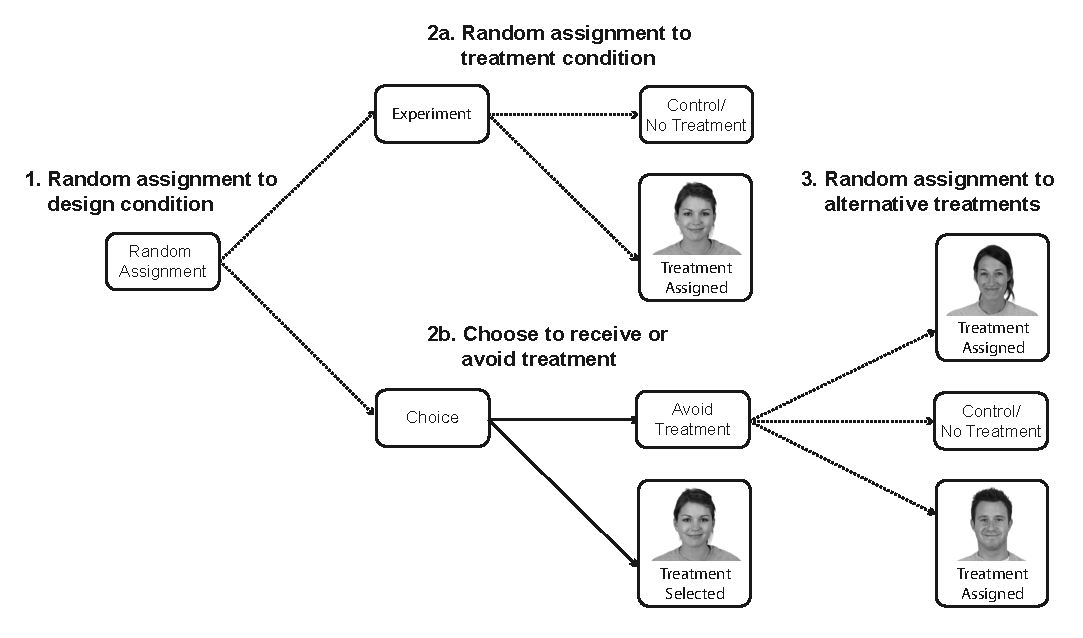
\includegraphics{design_simple_gs.pdf}

Note: Figure created using Adobe Illustrator

\setcounter{figure}{1}

\hypertarget{figure-2-statistical-power-with-more-selectors-than-avoiders-equal-and-offsetting-effects}{%
\subsection{Figure 2: Statistical Power with More Selectors than
Avoiders, Equal and Offsetting
Effects}\label{figure-2-statistical-power-with-more-selectors-than-avoiders-equal-and-offsetting-effects}}

\begin{Shaded}
\begin{Highlighting}[]
\CommentTok{\#Uncomment to run. 500 Simulation takes \textasciitilde{} 30{-}40 minutes}
\CommentTok{\# Set random seed}
\CommentTok{\#set.seed(123)}

\CommentTok{\#fig2\_power\_sim \textless{}{-} display\_power\_sim\_fn(}
\CommentTok{\#                       p\_s\_sims = 500,}
\CommentTok{\#                       p\_s\_prop\_select = 2/3,}
\CommentTok{\#                       p\_s\_tau\_st = seq(.1,.7,by=.05),}
\CommentTok{\#                       p\_s\_tau\_af = seq({-}.1,{-}.7,by={-}.05),}
\CommentTok{\#                       p\_s\_tau\_am = seq(.1,.7,by=.05)}
\CommentTok{\#                       )}
\CommentTok{\#print(fig2\_power\_sim)}

\CommentTok{\# Format Figure 2}
\NormalTok{fig2 }\OtherTok{\textless{}{-}}\NormalTok{ fig2\_power\_sim [[}\DecValTok{1}\NormalTok{]]}\SpecialCharTok{+}
  \FunctionTok{theme\_bw}\NormalTok{()}\SpecialCharTok{+}
  \FunctionTok{theme}\NormalTok{(}
    \AttributeTok{panel.grid.minor =} \FunctionTok{element\_blank}\NormalTok{(),}
\NormalTok{  )}\SpecialCharTok{+}
  \FunctionTok{scale\_color\_grey}\NormalTok{(}\AttributeTok{start =} \DecValTok{0}\NormalTok{, }\AttributeTok{end =}\NormalTok{ .}\DecValTok{75}\NormalTok{)}

\CommentTok{\# Display Figure 2}
\NormalTok{fig2}
\end{Highlighting}
\end{Shaded}

\begin{figure}
\centering
\includegraphics{Reproduction-of-original-code_w-simulations_files/figure-latex/fig2-1.pdf}
\caption{Statistical Power with More Selectors than Avoiders, Equal and
Offsetting Effects}
\end{figure}

\hypertarget{figure-3-who-is-likely-to-seek-out-or-avoid-the-message-of-the-metoo-movement}{%
\subsection{Figure 3: Who is Likely to Seek Out or Avoid the Message of
the \#MeToo
Movement?}\label{figure-3-who-is-likely-to-seek-out-or-avoid-the-message-of-the-metoo-movement}}

\begin{Shaded}
\begin{Highlighting}[]
\CommentTok{\# Create Figure 3}
\NormalTok{fig3 }\OtherTok{\textless{}{-}} \FunctionTok{plot\_balance\_fn}\NormalTok{(df\_mtg)}

\CommentTok{\# Display Figure 3}
\NormalTok{fig3}
\end{Highlighting}
\end{Shaded}

\begin{figure}
\centering
\includegraphics{Reproduction-of-original-code_w-simulations_files/figure-latex/fig3-1.pdf}
\caption{Who is Likely to Seek Out or Avoid the Message of the \#MeToo
Movement?}
\end{figure}

\hypertarget{figure-4-heterogeneous-effects-in-the-metoo-mturk-study}{%
\subsection{Figure 4: Heterogeneous Effects in the \#MeToo MTurk
Study}\label{figure-4-heterogeneous-effects-in-the-metoo-mturk-study}}

\begin{Shaded}
\begin{Highlighting}[]
\CommentTok{\# Create Figure 4}
\NormalTok{fig4 }\OtherTok{\textless{}{-}} \FunctionTok{plot\_effects\_fn}\NormalTok{(df\_mtg,}\StringTok{"dv\_pca\_metoo"}\NormalTok{) }\SpecialCharTok{+} \FunctionTok{scale\_color\_grey}\NormalTok{(}\AttributeTok{start =} \DecValTok{0}\NormalTok{, }\AttributeTok{end =}\NormalTok{ .}\DecValTok{75}\NormalTok{) }

\CommentTok{\# Display Figure 4}
\NormalTok{fig4}
\end{Highlighting}
\end{Shaded}

\begin{figure}
\centering
\includegraphics{Reproduction-of-original-code_w-simulations_files/figure-latex/fig4 -1.pdf}
\caption{Heterogeneous Effects in the \#MeToo MTurk Study}
\end{figure}

\hypertarget{figure-5-who-is-likely-to-seek-out-or-avoid-the-message-of-the-metoo-movement-in-a-more-nationally-representative-sample}{%
\subsection{Figure 5: Who is Likely to Seek Out or Avoid the Message of
the \#MeToo Movement in a More Nationally Representative
Sample?}\label{figure-5-who-is-likely-to-seek-out-or-avoid-the-message-of-the-metoo-movement-in-a-more-nationally-representative-sample}}

\begin{Shaded}
\begin{Highlighting}[]
\CommentTok{\# Create Figure 3}
\NormalTok{fig5 }\OtherTok{\textless{}{-}} \FunctionTok{plot\_balance\_fn}\NormalTok{(df\_qg)}

\CommentTok{\# Display Figure 3}
\NormalTok{fig5}
\end{Highlighting}
\end{Shaded}

\begin{figure}
\centering
\includegraphics{Reproduction-of-original-code_w-simulations_files/figure-latex/fig5-1.pdf}
\caption{Who Seeks Out or Avoids the Message of the \#MeToo Movement in
a More Nationally Representative Sample?}
\end{figure}

\hypertarget{figure-6-heterogeneous-effects-in-the-metoo-qualtrics-study}{%
\subsection{Figure 6: Heterogeneous Effects in the \#MeToo Qualtrics
Study}\label{figure-6-heterogeneous-effects-in-the-metoo-qualtrics-study}}

\begin{Shaded}
\begin{Highlighting}[]
\CommentTok{\# Create Figure 6}
\NormalTok{fig6 }\OtherTok{\textless{}{-}} \FunctionTok{plot\_effects\_fn}\NormalTok{(df\_qg,}\StringTok{"dv\_pca\_metoo"}\NormalTok{) }\SpecialCharTok{+} \FunctionTok{scale\_color\_grey}\NormalTok{(}\AttributeTok{start =} \DecValTok{0}\NormalTok{, }\AttributeTok{end =}\NormalTok{ .}\DecValTok{75}\NormalTok{) }

\CommentTok{\# Display Figure 6}
\NormalTok{fig6 }
\end{Highlighting}
\end{Shaded}

\begin{figure}
\centering
\includegraphics{Reproduction-of-original-code_w-simulations_files/figure-latex/fig6-1.pdf}
\caption{Heterogeneous Effects in the \#MeToo Qualtrics Study}
\end{figure}

\hypertarget{main-tables}{%
\section{Main Tables}\label{main-tables}}

\hypertarget{table-1}{%
\subsection{Table 1}\label{table-1}}

\begin{Shaded}
\begin{Highlighting}[]
\FunctionTok{table\_fn}\NormalTok{(fig4}\SpecialCharTok{$}\NormalTok{data,}
    \StringTok{"Table 1: Treatment Effect Estimates on Specific Support for }\SpecialCharTok{\textbackslash{}\textbackslash{}}\StringTok{\#MeToo (MTurk Sample)"}\NormalTok{)}
\end{Highlighting}
\end{Shaded}

\begin{table}[H]

\caption{\label{tab:tab1}Table 1: Treatment Effect Estimates on Specific Support for \#MeToo (MTurk Sample)}
\centering
\begin{threeparttable}
\begin{tabular}[t]{lccclc}
\toprule
 & Overall & Men & Women & Republicans & Democrats\\
\midrule
\addlinespace[0.3em]
\multicolumn{6}{l}{\textbf{ATE}}\\
\hspace{1em}ATE & 0.22 & 0.03 & 0.41 & 0.29 & 0.16\\
\hspace{1em} & {}[0.03, 0.41] & {}[-0.27, 0.33] & {}[0.18, 0.64] & {}[-0.10, 0.68] & {}[-0.05, 0.36]\\
\addlinespace[0.3em]
\multicolumn{6}{l}{\textbf{ACTE}}\\
\hspace{1em}Select Treatment & 0.19 & 0.02 & 0.33 & 0.07 & 0.18\\
\hspace{1em} & {}[-0.01, 0.39] & {}[-0.29, 0.32] & {}[0.08, 0.58] & {}[-0.35, 0.49] & {}[-0.02, 0.38]\\
\hspace{1em}Avoid Treatment & 0.37 & 0.09 & 0.83 & 1.04 & 0.04\\
\hspace{1em} & {}[-0.47, 1.20] & {}[-1.12, 1.30] & {}[-0.19, 1.84] & {}[-0.40, 2.48] & {}[-0.96, 1.03]\\
\addlinespace[0.3em]
\multicolumn{6}{l}{\textbf{CACTE}}\\
\hspace{1em}Female Treatment & 0.24 & 0.29 & 0.22 & 1.27 & -0.22\\
\hspace{1em} & {}[-0.27, 0.75] & {}[-0.38, 0.96] & {}[-0.57, 1.01] & {}[0.42, 2.12] & {}[-0.88, 0.45]\\
\hspace{1em}Male Treatment & 0.21 & 0.02 & 0.46 & 0.89 & -0.18\\
\hspace{1em} & {}[-0.32, 0.74] & {}[-0.76, 0.81] & {}[-0.14, 1.05] & {}[0.18, 1.60] & {}[-1.16, 0.81]\\
\bottomrule
\end{tabular}
\begin{tablenotes}
\small
\item \textit{Note: } 
\item The table provides point estimates and 95\% confidence intervals for treatment effect estimated from the full sample and separately by gender and partisanship
\end{tablenotes}
\end{threeparttable}
\end{table}

\hypertarget{table-2}{%
\subsection{Table 2}\label{table-2}}

\begin{Shaded}
\begin{Highlighting}[]
\FunctionTok{table\_fn}\NormalTok{(fig6}\SpecialCharTok{$}\NormalTok{data,}
    \StringTok{"Table 2: Treatment Effect Estimates on Specific Support for }\SpecialCharTok{\textbackslash{}\textbackslash{}}\StringTok{\#MeToo (Qualtrics Sample)"}\NormalTok{)}
\end{Highlighting}
\end{Shaded}

\begin{table}[H]

\caption{\label{tab:tab2}Table 2: Treatment Effect Estimates on Specific Support for \#MeToo (Qualtrics Sample)}
\centering
\begin{threeparttable}
\begin{tabular}[t]{lccclc}
\toprule
 & Overall & Men & Women & Republicans & Democrats\\
\midrule
\addlinespace[0.3em]
\multicolumn{6}{l}{\textbf{ATE}}\\
\hspace{1em}ATE & 0.29 & 0.29 & 0.28 & 0.09 & 0.18\\
\hspace{1em} & {}[0.10, 0.48] & {}[0.01, 0.58] & {}[0.03, 0.52] & {}[-0.27, 0.44] & {}[-0.06, 0.42]\\
\addlinespace[0.3em]
\multicolumn{6}{l}{\textbf{ACTE}}\\
\hspace{1em}Select Treatment & 0.24 & 0.35 & 0.14 & 0.08 & 0.19\\
\hspace{1em} & {}[-0.01, 0.49] & {}[-0.01, 0.71] & {}[-0.20, 0.48] & {}[-0.34, 0.49] & {}[-0.11, 0.49]\\
\hspace{1em}Avoid Treatment & 0.38 & 0.17 & 0.54 & 0.11 & 0.17\\
\hspace{1em} & {}[-0.09, 0.84] & {}[-0.58, 0.93] & {}[-0.03, 1.10] & {}[-0.99, 1.22] & {}[-0.47, 0.80]\\
\addlinespace[0.3em]
\multicolumn{6}{l}{\textbf{CACTE}}\\
\hspace{1em}Female Treatment & -0.23 & -0.48 & 0.15 & -0.32 & 0.09\\
\hspace{1em} & {}[-0.61, 0.14] & {}[-1.00, 0.05] & {}[-0.39, 0.69] & {}[-0.96, 0.32] & {}[-0.46, 0.64]\\
\hspace{1em}Male Treatment & 0.32 & 0.62 & 0.11 & 0.46 & 0.36\\
\hspace{1em} & {}[-0.05, 0.70] & {}[0.12, 1.11] & {}[-0.43, 0.64] & {}[-0.50, 1.42] & {}[-0.11, 0.84]\\
\bottomrule
\end{tabular}
\begin{tablenotes}
\small
\item \textit{Note: } 
\item The table provides point estimates and 95\% confidence intervals for treatment effect estimated from the full sample and separately by gender and partisanship
\end{tablenotes}
\end{threeparttable}
\end{table}

\hypertarget{online-appendix}{%
\section{Online Appendix}\label{online-appendix}}

\hypertarget{appendix-c-power-simulations}{%
\subsection{Appendix C Power
Simulations}\label{appendix-c-power-simulations}}

\setcounter{table}{0}
\renewcommand{\thetable}{C.\arabic{table}}
\setcounter{figure}{0}
\renewcommand{\thefigure}{C.\arabic{figure}}

\hypertarget{figure-and-table-c.1-statistical-power-with-equal-number-of-selectors-than-avoiders-equal-and-offsetting-effects}{%
\subsubsection{Figure and Table C.1: Statistical Power with Equal Number
of Selectors than Avoiders, Equal and Offsetting
Effects}\label{figure-and-table-c.1-statistical-power-with-equal-number-of-selectors-than-avoiders-equal-and-offsetting-effects}}

\begin{Shaded}
\begin{Highlighting}[]
\CommentTok{\# Uncomment to run. 500 Simulation takes \textasciitilde{} 30{-}40 minutes}
\CommentTok{\# Set random seed}
\CommentTok{\#set.seed(123)}

\CommentTok{\#figC1\_power\_sim \textless{}{-} display\_power\_sim\_fn(}
\CommentTok{\#                      p\_s\_sims = 500,}
\CommentTok{\#                       p\_s\_prop\_select = .5,}
\CommentTok{\#                       p\_s\_tau\_st = seq(.1,.7,by=.05),}
\CommentTok{\#                       p\_s\_tau\_af = seq({-}.1,{-}.7,by={-}.05),}
\CommentTok{\#                       p\_s\_tau\_am = seq(.1,.7,by=.05)}
\CommentTok{\#                       )}
\CommentTok{\#}
\CommentTok{\#figC1\_power\_sim[[1]]}
\end{Highlighting}
\end{Shaded}

\begin{Shaded}
\begin{Highlighting}[]
\NormalTok{figC1\_power\_sim[[}\DecValTok{2}\NormalTok{]]}
\end{Highlighting}
\end{Shaded}

\begin{table}[!h]

\caption{\label{tab:figpower1}Power Analysis}
\centering
\begin{tabular}[t]{lrrrrrrrrrrrrr}
\toprule
\multicolumn{1}{c}{} & \multicolumn{13}{c}{Hypothesized Effect Among Selectors} \\
\cmidrule(l{3pt}r{3pt}){2-14}
  & 0.1 & 0.15 & 0.2 & 0.25 & 0.3 & 0.35 & 0.4 & 0.45 & 0.5 & 0.55 & 0.6 & 0.65 & 0.7\\
\midrule
ATE & 0.05 & 0.06 & 0.05 & 0.05 & 0.04 & 0.05 & 0.05 & 0.05 & 0.06 & 0.04 & 0.04 & 0.06 & 0.06\\
ACTE-Select & 0.11 & 0.19 & 0.26 & 0.35 & 0.44 & 0.61 & 0.74 & 0.80 & 0.87 & 0.95 & 0.96 & 0.98 & 0.98\\
ACTE-Avoid & 0.09 & 0.15 & 0.24 & 0.28 & 0.39 & 0.49 & 0.59 & 0.65 & 0.77 & 0.78 & 0.85 & 0.90 & 0.89\\
CACTE-Female & NA & NA & NA & NA & NA & NA & NA & NA & NA & NA & NA & NA & NA\\
CACTE-Male & NA & NA & NA & NA & NA & NA & NA & NA & NA & NA & NA & NA & NA\\
\bottomrule
\end{tabular}
\end{table}

\hypertarget{figure-and-table-c.2-statistical-power-with-more-selectors-than-avoiders-equal-and-offsetting-effects}{%
\subsubsection{Figure and Table C.2: Statistical Power with More
Selectors than Avoiders, Equal and Offsetting
Effects}\label{figure-and-table-c.2-statistical-power-with-more-selectors-than-avoiders-equal-and-offsetting-effects}}

\begin{Shaded}
\begin{Highlighting}[]
\CommentTok{\# Same as Figure 2}
\NormalTok{fig2\_power\_sim[[}\DecValTok{1}\NormalTok{]]}
\end{Highlighting}
\end{Shaded}

\begin{figure}
\centering
\includegraphics{Reproduction-of-original-code_w-simulations_files/figure-latex/figpower2-1.pdf}
\caption{Statistical Power with More Selectors than Avoiders, Equal and
Offsetting Effects}
\end{figure}

\begin{Shaded}
\begin{Highlighting}[]
\NormalTok{fig2\_power\_sim[[}\DecValTok{2}\NormalTok{]]}
\end{Highlighting}
\end{Shaded}

\begin{table}[!h]

\caption{\label{tab:fig2}Power Analysis}
\centering
\begin{tabular}[t]{lrrrrrrrrrrrrr}
\toprule
\multicolumn{1}{c}{} & \multicolumn{13}{c}{Hypothesized Effect Among Selectors} \\
\cmidrule(l{3pt}r{3pt}){2-14}
  & 0.1 & 0.15 & 0.2 & 0.25 & 0.3 & 0.35 & 0.4 & 0.45 & 0.5 & 0.55 & 0.6 & 0.65 & 0.7\\
\midrule
ATE & 0.07 & 0.05 & 0.07 & 0.12 & 0.15 & 0.13 & 0.20 & 0.20 & 0.27 & 0.36 & 0.41 & 0.42 & 0.43\\
ACTE-Select & 0.13 & 0.20 & 0.41 & 0.53 & 0.68 & 0.78 & 0.91 & 0.94 & 0.97 & 0.99 & 1.00 & 1.00 & 1.00\\
ACTE-Avoid & 0.07 & 0.07 & 0.13 & 0.16 & 0.17 & 0.26 & 0.26 & 0.33 & 0.34 & 0.35 & 0.40 & 0.49 & 0.51\\
CACTE-Female & NA & NA & NA & NA & NA & NA & NA & NA & NA & NA & NA & NA & NA\\
CACTE-Male & NA & NA & NA & NA & NA & NA & NA & NA & NA & NA & NA & NA & NA\\
\bottomrule
\end{tabular}
\end{table}

\hypertarget{figure-and-table-c.3-statistical-power-with-more-selectors-than-avoiders-equal-and-offsetting-effects-and-selection-correlated-with-outcome}{%
\subsubsection{Figure and Table C.3: Statistical Power with More
Selectors than Avoiders, Equal and Offsetting Effects, and Selection
Correlated with
Outcome}\label{figure-and-table-c.3-statistical-power-with-more-selectors-than-avoiders-equal-and-offsetting-effects-and-selection-correlated-with-outcome}}

\begin{Shaded}
\begin{Highlighting}[]
\CommentTok{\# Uncomment to run. 500 Simulation takes \textasciitilde{} 30{-}40 minutes}

\CommentTok{\# Set random seed}
\CommentTok{\#set.seed(123)}

\CommentTok{\#figC3\_power\_sim \textless{}{-} display\_power\_sim\_fn(}
\CommentTok{\#                      p\_s\_sims = 500,}
\CommentTok{\#                       p\_s\_prop\_select = 2/3,}
\CommentTok{\#                       p\_s\_select\_effect = 0.5,}
\CommentTok{\#                       p\_s\_tau\_st = seq(.1,.7,by=.05),}
\CommentTok{\#                       p\_s\_tau\_af = seq({-}.1,{-}.7,by={-}.05),}
\CommentTok{\#                       p\_s\_tau\_am = seq(.1,.7,by=.05)}
\CommentTok{\#                       )}

\CommentTok{\#figC3\_power\_sim[[1]]}
\end{Highlighting}
\end{Shaded}

\begin{Shaded}
\begin{Highlighting}[]
\NormalTok{figC3\_power\_sim[[}\DecValTok{2}\NormalTok{]]}
\end{Highlighting}
\end{Shaded}

\begin{table}[!h]

\caption{\label{tab:figpower3}Power Analysis}
\centering
\begin{tabular}[t]{lrrrrrrrrrrrrr}
\toprule
\multicolumn{1}{c}{} & \multicolumn{13}{c}{Hypothesized Effect Among Selectors} \\
\cmidrule(l{3pt}r{3pt}){2-14}
  & 0.1 & 0.15 & 0.2 & 0.25 & 0.3 & 0.35 & 0.4 & 0.45 & 0.5 & 0.55 & 0.6 & 0.65 & 0.7\\
\midrule
ATE & 0.07 & 0.06 & 0.08 & 0.12 & 0.16 & 0.13 & 0.17 & 0.19 & 0.26 & 0.32 & 0.35 & 0.36 & 0.35\\
ACTE-Select & 0.12 & 0.19 & 0.38 & 0.50 & 0.65 & 0.75 & 0.89 & 0.92 & 0.95 & 0.99 & 1.00 & 1.00 & 1.00\\
ACTE-Avoid & 0.07 & 0.07 & 0.11 & 0.16 & 0.16 & 0.22 & 0.21 & 0.27 & 0.28 & 0.30 & 0.33 & 0.41 & 0.46\\
CACTE-Female & NA & NA & NA & NA & NA & NA & NA & NA & NA & NA & NA & NA & NA\\
CACTE-Male & NA & NA & NA & NA & NA & NA & NA & NA & NA & NA & NA & NA & NA\\
\bottomrule
\end{tabular}
\end{table}

\begin{Shaded}
\begin{Highlighting}[]
\CommentTok{\# Uncomment to save results of power simulations}
\CommentTok{\#save(figC1\_power\_sim, fig2\_power\_sim,figC3\_power\_sim,file = "power\_simulations.rda")}
\end{Highlighting}
\end{Shaded}

\hypertarget{appendix-d-descriptive-statistics}{%
\subsection{Appendix D Descriptive
Statistics}\label{appendix-d-descriptive-statistics}}

\setcounter{table}{0}
\renewcommand{\thetable}{D.\arabic{table}}
\setcounter{figure}{0}
\renewcommand{\thefigure}{D.\arabic{figure}}

\hypertarget{table-d.1-descriptive-statistics-for-mturk-sample}{%
\subsubsection{Table D.1: Descriptive Statistics for MTurk
Sample}\label{table-d.1-descriptive-statistics-for-mturk-sample}}

\begin{Shaded}
\begin{Highlighting}[]
\NormalTok{the\_covariates }\OtherTok{\textless{}{-}} \FunctionTok{c}\NormalTok{(}\StringTok{"female01"}\NormalTok{, }\StringTok{"age"}\NormalTok{, }\StringTok{"income"}\NormalTok{, }\StringTok{"education"}\NormalTok{, }\StringTok{"pid"}\NormalTok{, }\StringTok{"ideo"}\NormalTok{, }
                    \StringTok{"black"}\NormalTok{, }\StringTok{"latino"}\NormalTok{, }\StringTok{"asian"}\NormalTok{, }\StringTok{"fam\_movement"}\NormalTok{, }\StringTok{"avoid01"}\NormalTok{)}
\NormalTok{desc\_tab\_mt}\OtherTok{\textless{}{-}} \FunctionTok{c}\NormalTok{()}
\ControlFlowTok{for}\NormalTok{(i }\ControlFlowTok{in} \DecValTok{1}\SpecialCharTok{:}\FunctionTok{length}\NormalTok{(the\_covariates))\{}
\NormalTok{  desc\_tab\_mt }\OtherTok{\textless{}{-}} \FunctionTok{cbind}\NormalTok{(desc\_tab\_mt,}
                       \FunctionTok{summary}\NormalTok{(df\_mtg[,the\_covariates[i]])[}\DecValTok{1}\SpecialCharTok{:}\DecValTok{6}\NormalTok{]}
\NormalTok{                       )}
\NormalTok{\}}
\NormalTok{desc\_tab\_mt }\OtherTok{\textless{}{-}} \FunctionTok{t}\NormalTok{(}\FunctionTok{round}\NormalTok{(desc\_tab\_mt,}\DecValTok{2}\NormalTok{))}
\FunctionTok{rownames}\NormalTok{(desc\_tab\_mt) }\OtherTok{\textless{}{-}} \FunctionTok{c}\NormalTok{(}\StringTok{"Prop. Female"}\NormalTok{, }\StringTok{"Age"}\NormalTok{, }\StringTok{"Income"}\NormalTok{, }\StringTok{"Education"}\NormalTok{,}
                           \StringTok{"Party ID"}\NormalTok{, }\StringTok{"Ideology"}\NormalTok{,}
                           \StringTok{"Prop. Black"}\NormalTok{,}
                           \StringTok{"Prop. Latinx"}\NormalTok{,}
                           \StringTok{"Prop. Asian"}\NormalTok{,}
                           \StringTok{"Familiarity with MeToo"}\NormalTok{,}
                           \StringTok{"Prop Avoiding Treatment"}\NormalTok{)}


\NormalTok{desc\_tab\_mt\_tex }\OtherTok{\textless{}{-}} \FunctionTok{kable}\NormalTok{(desc\_tab\_mt,}
      \AttributeTok{booktabs =} \ConstantTok{TRUE}\NormalTok{, }
               \AttributeTok{caption =} \StringTok{"Descriptive Statistics for MTurk Sample"}\NormalTok{, }
               \AttributeTok{digits=}\DecValTok{2}\NormalTok{,}
  \AttributeTok{align =} \StringTok{"l"}\NormalTok{) }\SpecialCharTok{\%\textgreater{}\%} 
  \FunctionTok{kable\_styling}\NormalTok{(}\AttributeTok{latex\_options =} \FunctionTok{c}\NormalTok{(}\StringTok{"hold\_position"}\NormalTok{,}\AttributeTok{font\_size=}\DecValTok{10}\NormalTok{))}
\NormalTok{desc\_tab\_mt\_tex}
\end{Highlighting}
\end{Shaded}

\begin{table}[!h]

\caption{\label{tab:tabD1}Descriptive Statistics for MTurk Sample}
\centering
\begin{tabular}[t]{lllllll}
\toprule
  & Min. & 1st Qu. & Median & Mean & 3rd Qu. & Max.\\
\midrule
Prop. Female & 0 & 0 & 0 & 0.49 & 1 & 1\\
Age & 18 & 29 & 35 & 38.12 & 45 & 82\\
Income & 1 & 4 & 6 & 6.23 & 8 & 12\\
Education & 1 & 3 & 5 & 4.31 & 5 & 7\\
Party ID & 1 & 2 & 3 & 3.49 & 6 & 7\\
\addlinespace
Ideology & 1 & 2 & 3 & 3.53 & 5 & 7\\
Prop. Black & 0 & 0 & 0 & 0.06 & 0 & 1\\
Prop. Latinx & 0 & 0 & 0 & 0.07 & 0 & 1\\
Prop. Asian & 0 & 0 & 0 & 0.09 & 0 & 1\\
Familiarity with MeToo & 0 & 2 & 3 & 2.45 & 3 & 4\\
\addlinespace
Prop Avoiding Treatment & 0 & 0 & 0 & 0.19 & 0 & 1\\
\bottomrule
\end{tabular}
\end{table}

\hypertarget{table-d.2-descriptive-statistics-for-qualtrics-sample}{%
\subsubsection{Table D.2: Descriptive Statistics for Qualtrics
Sample}\label{table-d.2-descriptive-statistics-for-qualtrics-sample}}

\begin{Shaded}
\begin{Highlighting}[]
\NormalTok{desc\_tab\_q }\OtherTok{\textless{}{-}} \FunctionTok{c}\NormalTok{()}
\NormalTok{df\_qg }\OtherTok{\textless{}{-}} \FunctionTok{data.frame}\NormalTok{(df\_qg)}
\ControlFlowTok{for}\NormalTok{(i }\ControlFlowTok{in} \DecValTok{1}\SpecialCharTok{:}\FunctionTok{length}\NormalTok{(the\_covariates))\{}
\NormalTok{  desc\_tab\_q }\OtherTok{\textless{}{-}} \FunctionTok{cbind}\NormalTok{(desc\_tab\_q,}
                       \FunctionTok{summary}\NormalTok{(}\FunctionTok{na.omit}\NormalTok{(df\_qg[,the\_covariates[i]])))}
                       
\NormalTok{\}}
\NormalTok{desc\_tab\_q }\OtherTok{\textless{}{-}} \FunctionTok{t}\NormalTok{(}\FunctionTok{round}\NormalTok{(desc\_tab\_q,}\DecValTok{2}\NormalTok{))}
\FunctionTok{rownames}\NormalTok{(desc\_tab\_q) }\OtherTok{\textless{}{-}} \FunctionTok{c}\NormalTok{(}\StringTok{"Prop. Female"}\NormalTok{, }\StringTok{"Age"}\NormalTok{, }\StringTok{"Income"}\NormalTok{, }\StringTok{"Education"}\NormalTok{,}
                           \StringTok{"Party ID"}\NormalTok{, }\StringTok{"Ideology"}\NormalTok{,}
                           \StringTok{"Prop. Black"}\NormalTok{,}
                           \StringTok{"Prop. Latinx"}\NormalTok{,}
                           \StringTok{"Prop. Asian"}\NormalTok{,}
                           \StringTok{"Familiarity with MeToo"}\NormalTok{,}
                           \StringTok{"Prop Avoiding Treatment"}\NormalTok{)}



\NormalTok{desc\_tab\_q\_tex }\OtherTok{\textless{}{-}} \FunctionTok{kable}\NormalTok{(desc\_tab\_q,}
      \AttributeTok{booktabs =} \ConstantTok{TRUE}\NormalTok{, }
               \AttributeTok{caption =} \StringTok{"Descriptive Statistics for Qualtrics Sample"}\NormalTok{, }
               \AttributeTok{digits=}\DecValTok{2}\NormalTok{,}
  \AttributeTok{align =} \StringTok{"l"}\NormalTok{) }\SpecialCharTok{\%\textgreater{}\%} 
  \FunctionTok{kable\_styling}\NormalTok{(}\AttributeTok{latex\_options =} \FunctionTok{c}\NormalTok{(}\StringTok{"hold\_position"}\NormalTok{,}\AttributeTok{font\_size=}\DecValTok{10}\NormalTok{))}
\NormalTok{desc\_tab\_q\_tex}
\end{Highlighting}
\end{Shaded}

\begin{table}[!h]

\caption{\label{tab:tabD2}Descriptive Statistics for Qualtrics Sample}
\centering
\begin{tabular}[t]{lllllll}
\toprule
  & Min. & 1st Qu. & Median & Mean & 3rd Qu. & Max.\\
\midrule
Prop. Female & 0 & 0 & 1 & 0.51 & 1 & 1\\
Age & 18 & 31 & 46 & 45.94 & 60 & 93\\
Income & 1 & 3 & 5 & 5.38 & 8 & 12\\
Education & 1 & 2 & 3 & 3.28 & 5 & 7\\
Party ID & 1 & 2 & 4 & 3.62 & 6 & 7\\
\addlinespace
Ideology & 1 & 3 & 4 & 4.04 & 5 & 7\\
Prop. Black & 0 & 0 & 0 & 0.17 & 0 & 1\\
Prop. Latinx & 0 & 0 & 0 & 0.18 & 0 & 1\\
Prop. Asian & 0 & 0 & 0 & 0.06 & 0 & 1\\
Familiarity with MeToo & 0 & 1 & 2 & 2.05 & 3 & 4\\
\addlinespace
Prop Avoiding Treatment & 0 & 0 & 0 & 0.33 & 1 & 1\\
\bottomrule
\end{tabular}
\end{table}

\hypertarget{appendix-e-effects-on-general-support-for-gender-equality}{%
\subsection{Appendix E Effects on General Support for Gender
Equality}\label{appendix-e-effects-on-general-support-for-gender-equality}}

\setcounter{table}{0}
\renewcommand{\thetable}{E.\arabic{table}}
\setcounter{figure}{0}
\renewcommand{\thefigure}{E.\arabic{figure}}

\hypertarget{figure-and-table-e.1-effects-on-general-support-for-gender-equality-mturk-study}{%
\subsubsection{Figure and Table E.1: Effects on General Support for
Gender Equality (MTurk
Study)}\label{figure-and-table-e.1-effects-on-general-support-for-gender-equality-mturk-study}}

\begin{Shaded}
\begin{Highlighting}[]
\CommentTok{\# Create Figure E1}
\NormalTok{figE1 }\OtherTok{\textless{}{-}} \FunctionTok{plot\_effects\_fn}\NormalTok{(df\_mtg, }\StringTok{"dv\_pca\_general"}\NormalTok{)}

\CommentTok{\# Display Figure 4}
\NormalTok{figE1 }
\end{Highlighting}
\end{Shaded}

\begin{figure}
\centering
\includegraphics{Reproduction-of-original-code_w-simulations_files/figure-latex/figE1-1.pdf}
\caption{Effects on General Support for Gender Equality (MTurk Study)}
\end{figure}

\begin{Shaded}
\begin{Highlighting}[]
\FunctionTok{table\_fn}\NormalTok{(figE1}\SpecialCharTok{$}\NormalTok{data,}
  \StringTok{"Treatment Effect Estimates on General Support for Gender Equality (MTurk Sample)"}
\NormalTok{  )}
\end{Highlighting}
\end{Shaded}

\begin{table}[H]

\caption{\label{tab:tabE1}Treatment Effect Estimates on General Support for Gender Equality (MTurk Sample)}
\centering
\begin{threeparttable}
\begin{tabular}[t]{lccclc}
\toprule
 & Overall & Men & Women & Republicans & Democrats\\
\midrule
\addlinespace[0.3em]
\multicolumn{6}{l}{\textbf{ATE}}\\
\hspace{1em}ATE & -0.04 & -0.02 & -0.05 & -0.08 & -0.01\\
\hspace{1em} & {}[-0.23, 0.15] & {}[-0.31, 0.27] & {}[-0.28, 0.19] & {}[-0.41, 0.26] & {}[-0.24, 0.21]\\
\addlinespace[0.3em]
\multicolumn{6}{l}{\textbf{ACTE}}\\
\hspace{1em}Select Treatment & -0.06 & -0.12 & 0.02 & -0.21 & 0.03\\
\hspace{1em} & {}[-0.23, 0.12] & {}[-0.40, 0.16] & {}[-0.19, 0.23] & {}[-0.58, 0.15] & {}[-0.15, 0.21]\\
\hspace{1em}Avoid Treatment & 0.01 & 0.36 & -0.38 & 0.41 & -0.24\\
\hspace{1em} & {}[-0.87, 0.90] & {}[-0.88, 1.61] & {}[-1.58, 0.81] & {}[-0.94, 1.76] & {}[-1.51, 1.03]\\
\addlinespace[0.3em]
\multicolumn{6}{l}{\textbf{CACTE}}\\
\hspace{1em}Female Treatment & 0.29 & 0.22 & 0.40 & 0.93 & -0.00\\
\hspace{1em} & {}[-0.18, 0.77] & {}[-0.44, 0.89] & {}[-0.21, 1.00] & {}[0.04, 1.83] & {}[-0.58, 0.58]\\
\hspace{1em}Male Treatment & -0.09 & -0.33 & 0.20 & 0.38 & -0.31\\
\hspace{1em} & {}[-0.65, 0.47] & {}[-1.12, 0.46] & {}[-0.44, 0.84] & {}[-0.42, 1.18] & {}[-1.32, 0.71]\\
\bottomrule
\end{tabular}
\begin{tablenotes}
\small
\item \textit{Note: } 
\item The table provides point estimates and 95\% confidence intervals for treatment effect estimated from the full sample and separately by gender and partisanship
\end{tablenotes}
\end{threeparttable}
\end{table}

\hypertarget{figure-and-table-e.2-effects-on-general-support-for-gender-equality-qualtrics-study}{%
\subsubsection{Figure and Table E.2: Effects on General Support for
Gender Equality (Qualtrics
Study)}\label{figure-and-table-e.2-effects-on-general-support-for-gender-equality-qualtrics-study}}

\begin{Shaded}
\begin{Highlighting}[]
\CommentTok{\# Create Figure E2}
\NormalTok{figE2 }\OtherTok{\textless{}{-}} \FunctionTok{plot\_effects\_fn}\NormalTok{(df\_qg, }\StringTok{"dv\_pca\_general"}\NormalTok{)}

\CommentTok{\# Display Figure E2}
\NormalTok{figE2 }
\end{Highlighting}
\end{Shaded}

\begin{figure}
\centering
\includegraphics{Reproduction-of-original-code_w-simulations_files/figure-latex/figE2-1.pdf}
\caption{Effects on General Support for Gender Equality (Qualtrics
Study)}
\end{figure}

\begin{Shaded}
\begin{Highlighting}[]
\FunctionTok{table\_fn}\NormalTok{(figE2}\SpecialCharTok{$}\NormalTok{data,}
  \StringTok{"Treatment Effect Estimates on General Support for Gender Equality (MTurk Sample)"}
\NormalTok{  )}
\end{Highlighting}
\end{Shaded}

\begin{table}[H]

\caption{\label{tab:tabE2}Treatment Effect Estimates on General Support for Gender Equality (MTurk Sample)}
\centering
\begin{threeparttable}
\begin{tabular}[t]{lccclc}
\toprule
 & Overall & Men & Women & Republicans & Democrats\\
\midrule
\addlinespace[0.3em]
\multicolumn{6}{l}{\textbf{ATE}}\\
\hspace{1em}ATE & 0.17 & 0.15 & 0.18 & 0.16 & 0.16\\
\hspace{1em} & {}[-0.03, 0.36] & {}[-0.12, 0.42] & {}[-0.10, 0.46] & {}[-0.13, 0.45] & {}[-0.14, 0.46]\\
\addlinespace[0.3em]
\multicolumn{6}{l}{\textbf{ACTE}}\\
\hspace{1em}Select Treatment & 0.21 & 0.04 & 0.38 & 0.21 & 0.22\\
\hspace{1em} & {}[-0.03, 0.44] & {}[-0.29, 0.36] & {}[0.04, 0.73] & {}[-0.12, 0.53] & {}[-0.12, 0.56]\\
\hspace{1em}Avoid Treatment & 0.09 & 0.39 & -0.19 & 0.05 & 0.02\\
\hspace{1em} & {}[-0.42, 0.60] & {}[-0.35, 1.14] & {}[-0.89, 0.50] & {}[-0.85, 0.95] & {}[-0.82, 0.87]\\
\addlinespace[0.3em]
\multicolumn{6}{l}{\textbf{CACTE}}\\
\hspace{1em}Female Treatment & -0.02 & -0.09 & 0.14 & 0.33 & -0.08\\
\hspace{1em} & {}[-0.36, 0.33] & {}[-0.57, 0.40] & {}[-0.40, 0.69] & {}[-0.27, 0.92] & {}[-0.58, 0.42]\\
\hspace{1em}Male Treatment & 0.01 & 0.05 & -0.02 & -0.35 & 0.30\\
\hspace{1em} & {}[-0.37, 0.39] & {}[-0.63, 0.74] & {}[-0.48, 0.44] & {}[-1.00, 0.30] & {}[-0.25, 0.84]\\
\bottomrule
\end{tabular}
\begin{tablenotes}
\small
\item \textit{Note: } 
\item The table provides point estimates and 95\% confidence intervals for treatment effect estimated from the full sample and separately by gender and partisanship
\end{tablenotes}
\end{threeparttable}
\end{table}

\hypertarget{f-additional-analyses}{%
\subsection{F Additional Analyses}\label{f-additional-analyses}}

\setcounter{table}{0}
\renewcommand{\thetable}{F.\arabic{table}}
\setcounter{figure}{0}
\renewcommand{\thefigure}{F.\arabic{figure}}

\hypertarget{figure-and-table-f.1-treatment-effect-estimates-on-specific-support-for-metoo-conditional-on-familiarity-and-gender-mturk-sample}{%
\subsubsection{Figure and Table F.1: Treatment Effect Estimates on
Specific Support for \#MeToo Conditional on Familiarity and Gender
(MTurk
Sample)}\label{figure-and-table-f.1-treatment-effect-estimates-on-specific-support-for-metoo-conditional-on-familiarity-and-gender-mturk-sample}}

\begin{Shaded}
\begin{Highlighting}[]
\NormalTok{figF1\_df }\OtherTok{\textless{}{-}} \FunctionTok{rbind}\NormalTok{(}
  \FunctionTok{data.frame}\NormalTok{(}
  \FunctionTok{effects\_fn}\NormalTok{(df\_mtg[df\_mtg}\SpecialCharTok{$}\NormalTok{fam\_movement}\SpecialCharTok{\textgreater{}}\DecValTok{2}\NormalTok{,], }\StringTok{"dv\_pca\_metoo"}\NormalTok{),}
  \AttributeTok{Group =} \StringTok{"Familiar"}\NormalTok{,}
  \AttributeTok{Type =} \StringTok{"By Familiarity"}\NormalTok{),}
  \FunctionTok{data.frame}\NormalTok{(}
  \FunctionTok{effects\_fn}\NormalTok{(df\_mtg[df\_mtg}\SpecialCharTok{$}\NormalTok{fam\_movement}\SpecialCharTok{\textless{}}\DecValTok{3}\NormalTok{,], }\StringTok{"dv\_pca\_metoo"}\NormalTok{),}
  \AttributeTok{Group =} \StringTok{"Unfamiliar"}\NormalTok{,}
  \AttributeTok{Type =} \StringTok{"By Familiarity"}\NormalTok{),}
  \FunctionTok{data.frame}\NormalTok{(}
  \FunctionTok{effects\_fn}\NormalTok{(df\_mtg[df\_mtg}\SpecialCharTok{$}\NormalTok{fam\_movement}\SpecialCharTok{\textgreater{}}\DecValTok{2} \SpecialCharTok{\&}\NormalTok{ df\_mtg}\SpecialCharTok{$}\NormalTok{gender}\SpecialCharTok{==}\DecValTok{0}\NormalTok{,], }\StringTok{"dv\_pca\_metoo"}\NormalTok{),}
  \AttributeTok{Group =} \StringTok{"Familiar"}\NormalTok{,}
  \AttributeTok{Type =} \StringTok{"Men"}\NormalTok{),}
  \FunctionTok{data.frame}\NormalTok{(}
  \FunctionTok{effects\_fn}\NormalTok{(df\_mtg[df\_mtg}\SpecialCharTok{$}\NormalTok{fam\_movement}\SpecialCharTok{\textless{}}\DecValTok{3}\SpecialCharTok{\&}\NormalTok{ df\_mtg}\SpecialCharTok{$}\NormalTok{gender}\SpecialCharTok{==}\DecValTok{0}\NormalTok{,], }\StringTok{"dv\_pca\_metoo"}\NormalTok{),}
  \AttributeTok{Group =} \StringTok{"Unfamiliar"}\NormalTok{,}
  \AttributeTok{Type =} \StringTok{"Men"}\NormalTok{),}
    \FunctionTok{data.frame}\NormalTok{(}
  \FunctionTok{effects\_fn}\NormalTok{(df\_mtg[df\_mtg}\SpecialCharTok{$}\NormalTok{fam\_movement}\SpecialCharTok{\textgreater{}}\DecValTok{2} \SpecialCharTok{\&}\NormalTok{ df\_mtg}\SpecialCharTok{$}\NormalTok{gender}\SpecialCharTok{==}\DecValTok{1}\NormalTok{,], }\StringTok{"dv\_pca\_metoo"}\NormalTok{),}
  \AttributeTok{Group =} \StringTok{"Familiar"}\NormalTok{,}
  \AttributeTok{Type =} \StringTok{"Women"}\NormalTok{),}
  \FunctionTok{data.frame}\NormalTok{(}
  \FunctionTok{effects\_fn}\NormalTok{(df\_mtg[df\_mtg}\SpecialCharTok{$}\NormalTok{fam\_movement}\SpecialCharTok{\textless{}}\DecValTok{3}\SpecialCharTok{\&}\NormalTok{ df\_mtg}\SpecialCharTok{$}\NormalTok{gender}\SpecialCharTok{==}\DecValTok{1}\NormalTok{,], }\StringTok{"dv\_pca\_metoo"}\NormalTok{),}
  \AttributeTok{Group =} \StringTok{"Unfamiliar"}\NormalTok{,}
  \AttributeTok{Type =} \StringTok{"Women"}\NormalTok{)}
\NormalTok{  )}

\NormalTok{figF1 }\OtherTok{\textless{}{-}}\NormalTok{ figF1\_df }\SpecialCharTok{\%\textgreater{}\%}
  \FunctionTok{filter}\NormalTok{(Estimand }\SpecialCharTok{!=} \StringTok{"CATE"}\NormalTok{)}\SpecialCharTok{\%\textgreater{}\%}
  \FunctionTok{ggplot}\NormalTok{(}\FunctionTok{aes}\NormalTok{(Estimate, Difference,}\AttributeTok{col=}\NormalTok{Group,}\AttributeTok{shape=}\NormalTok{Group))}\SpecialCharTok{+}
  \FunctionTok{geom\_hline}\NormalTok{(}\AttributeTok{yintercept =} \DecValTok{0}\NormalTok{,}\AttributeTok{linetype=}\StringTok{"dashed"}\NormalTok{,}\AttributeTok{alpha=}\NormalTok{.}\DecValTok{5}\NormalTok{)}\SpecialCharTok{+}
  \FunctionTok{facet\_grid}\NormalTok{(}\SpecialCharTok{\textasciitilde{}}\NormalTok{Type)}\SpecialCharTok{+}
  \FunctionTok{geom\_point}\NormalTok{(}\FunctionTok{aes}\NormalTok{(}\AttributeTok{shape=}\NormalTok{Group),}
                 \AttributeTok{position =} \FunctionTok{position\_dodge}\NormalTok{(}\AttributeTok{width =}\NormalTok{ .}\DecValTok{5}\NormalTok{),}\AttributeTok{size=}\DecValTok{2}
\NormalTok{      )}\SpecialCharTok{+}
  \FunctionTok{geom\_linerange}\NormalTok{(}\FunctionTok{aes}\NormalTok{(}\AttributeTok{ymin=}\NormalTok{ll,}\AttributeTok{ymax=}\NormalTok{ul),}\AttributeTok{size=}\NormalTok{.}\DecValTok{3}\NormalTok{,}
                       \AttributeTok{position =} \FunctionTok{position\_dodge}\NormalTok{(}\AttributeTok{width =}\NormalTok{ .}\DecValTok{5}\NormalTok{))}\SpecialCharTok{+}
  \FunctionTok{geom\_linerange}\NormalTok{(}\FunctionTok{aes}\NormalTok{(}\AttributeTok{ymin=}\NormalTok{ll90,}\AttributeTok{ymax=}\NormalTok{ul90),}\AttributeTok{size=}\NormalTok{.}\DecValTok{6}\NormalTok{,}
                     \AttributeTok{position =} \FunctionTok{position\_dodge}\NormalTok{(}\AttributeTok{width =}\NormalTok{ .}\DecValTok{5}\NormalTok{))}\SpecialCharTok{+}
  \FunctionTok{coord\_flip}\NormalTok{()}\SpecialCharTok{+}
  \FunctionTok{theme\_bw}\NormalTok{()}\SpecialCharTok{+}
  \FunctionTok{theme}\NormalTok{(}
    \AttributeTok{panel.grid.minor =} \FunctionTok{element\_blank}\NormalTok{(),}
    \AttributeTok{legend.position =} \StringTok{"bottom"}
\NormalTok{  )}

\NormalTok{figF1}
\end{Highlighting}
\end{Shaded}

\begin{figure}
\centering
\includegraphics{Reproduction-of-original-code_w-simulations_files/figure-latex/figF1-1.pdf}
\caption{Treatment Effect Estimates on Specific Support for \#MeToo
Conditional on Familiarity and Gender}
\end{figure}

\begin{Shaded}
\begin{Highlighting}[]
\CommentTok{\# Create Grouping Label }
\CommentTok{\#df\_mtg$Familiarity \textless{}{-} ifelse(df\_mtg$fam\_movement\textgreater{}2, "Familiar", "Unfamiliar")}

\FunctionTok{table\_app\_fn}\NormalTok{(df\_mtg, }\StringTok{"dv\_pca\_metoo"}\NormalTok{,}
         \StringTok{"Familiarity"}\NormalTok{,}
\NormalTok{         Familiarity,}
         \AttributeTok{the\_cap =}\StringTok{"Treatment Effect Estimates on Specific Support for }\SpecialCharTok{\textbackslash{}\textbackslash{}}\StringTok{\#MeToo Conditional On Familiarity and Gender (MTurk Sample)"}\NormalTok{ )}\SpecialCharTok{\%\textgreater{}\%}
  \FunctionTok{footnote}\NormalTok{(}\AttributeTok{general =} \StringTok{"The table provides point estimates and 95\% confidence intervals for treatment effect estimated by level of pre{-}test familiarity with the movement overall and by gender"}\NormalTok{,}
           \AttributeTok{threeparttable =}\NormalTok{ T,}
           \AttributeTok{fixed\_small\_size =}\NormalTok{ T)}
\end{Highlighting}
\end{Shaded}

\begin{table}[H]

\caption{\label{tab:tabF1}Treatment Effect Estimates on Specific Support for \#MeToo Conditional On Familiarity and Gender (MTurk Sample)}
\centering
\begin{threeparttable}
\begin{tabular}[t]{lcccccc}
\toprule
\multicolumn{1}{c}{ } & \multicolumn{2}{c}{Full Sample} & \multicolumn{2}{c}{Men} & \multicolumn{2}{c}{Women} \\
\cmidrule(l{3pt}r{3pt}){2-3} \cmidrule(l{3pt}r{3pt}){4-5} \cmidrule(l{3pt}r{3pt}){6-7}
  & Familiar & Unfamiliar & Familiar & Unfamiliar & Familiar & Unfamiliar\\
\midrule
\addlinespace[0.3em]
\multicolumn{7}{l}{\textbf{ATE}}\\
\hspace{1em}ATE & 0.13 & 0.36 & 0.08 & -0.01 & 0.16 & 0.75\\
\hspace{1em} & {}[-0.14, 0.39] & {}[0.09, 0.64] & {}[-0.33, 0.50] & {}[-0.44, 0.43] & {}[-0.14, 0.46] & {}[0.42, 1.08]\\
\addlinespace[0.3em]
\multicolumn{7}{l}{\textbf{ACTE}}\\
\hspace{1em}Select Treatment & 0.04 & 0.40 & -0.10 & 0.17 & 0.12 & 0.64\\
\hspace{1em} & {}[-0.23, 0.30] & {}[0.11, 0.68] & {}[-0.53, 0.33] & {}[-0.26, 0.60] & {}[-0.19, 0.43] & {}[0.26, 1.01]\\
\hspace{1em}Avoid Treatment & 0.57 & 0.23 & 0.87 & -0.63 & 0.38 & 1.22\\
\hspace{1em} & {}[-0.71, 1.85] & {}[-0.84, 1.30] & {}[-0.99, 2.74] & {}[-2.22, 0.95] & {}[-1.20, 1.96] & {}[-0.08, 2.51]\\
\addlinespace[0.3em]
\multicolumn{7}{l}{\textbf{CACTE}}\\
\hspace{1em}Female Treatment & 0.57 & 0.03 & 1.22 & -0.01 & -0.15 & 0.44\\
\hspace{1em} & {}[-0.29, 1.42] & {}[-0.57, 0.63] & {}[-0.04, 2.48] & {}[-0.78, 0.77] & {}[-1.39, 1.10] & {}[-0.85, 1.74]\\
\hspace{1em}Male Treatment & -0.05 & 0.47 & -0.26 & 0.37 & 0.24 & 0.57\\
\hspace{1em} & {}[-0.90, 0.79] & {}[-0.22, 1.16] & {}[-1.39, 0.87] & {}[-0.82, 1.57] & {}[-0.78, 1.26] & {}[-0.24, 1.37]\\
\bottomrule
\end{tabular}
\begin{tablenotes}
\small
\item \textit{Note: } 
\item The table provides point estimates and 95\% confidence intervals for treatment effect estimated by level of pre-test familiarity with the movement overall and by gender
\end{tablenotes}
\end{threeparttable}
\end{table}

\hypertarget{figure-and-table-f.2-treatment-effect-estimates-on-specific-support-for-metoo-conditional-on-familiarity-and-gender-qualtrics-study}{%
\subsubsection{Figure and Table F.2: Treatment Effect Estimates on
Specific Support for \#MeToo Conditional on Familiarity and Gender
(Qualtrics
Study)}\label{figure-and-table-f.2-treatment-effect-estimates-on-specific-support-for-metoo-conditional-on-familiarity-and-gender-qualtrics-study}}

\begin{Shaded}
\begin{Highlighting}[]
\NormalTok{figF2\_df }\OtherTok{\textless{}{-}} \FunctionTok{rbind}\NormalTok{(}
  \FunctionTok{data.frame}\NormalTok{(}
  \FunctionTok{effects\_fn}\NormalTok{(df\_qg[df\_qg}\SpecialCharTok{$}\NormalTok{fam\_movement}\SpecialCharTok{\textgreater{}}\DecValTok{2}\NormalTok{,], }\StringTok{"dv\_pca\_metoo"}\NormalTok{),}
  \AttributeTok{Group =} \StringTok{"Familiar"}\NormalTok{,}
  \AttributeTok{Type =} \StringTok{"By Familiarity"}\NormalTok{),}
  \FunctionTok{data.frame}\NormalTok{(}
  \FunctionTok{effects\_fn}\NormalTok{(df\_qg[df\_qg}\SpecialCharTok{$}\NormalTok{fam\_movement}\SpecialCharTok{\textless{}}\DecValTok{3}\NormalTok{,], }\StringTok{"dv\_pca\_metoo"}\NormalTok{),}
  \AttributeTok{Group =} \StringTok{"Unfamiliar"}\NormalTok{,}
  \AttributeTok{Type =} \StringTok{"By Familiarity"}\NormalTok{),}
  \FunctionTok{data.frame}\NormalTok{(}
  \FunctionTok{effects\_fn}\NormalTok{(df\_qg[df\_qg}\SpecialCharTok{$}\NormalTok{fam\_movement}\SpecialCharTok{\textgreater{}}\DecValTok{2} \SpecialCharTok{\&}\NormalTok{ df\_qg}\SpecialCharTok{$}\NormalTok{gender}\SpecialCharTok{==}\DecValTok{0}\NormalTok{,], }\StringTok{"dv\_pca\_metoo"}\NormalTok{),}
  \AttributeTok{Group =} \StringTok{"Familiar"}\NormalTok{,}
  \AttributeTok{Type =} \StringTok{"Men"}\NormalTok{),}
  \FunctionTok{data.frame}\NormalTok{(}
  \FunctionTok{effects\_fn}\NormalTok{(df\_qg[df\_qg}\SpecialCharTok{$}\NormalTok{fam\_movement}\SpecialCharTok{\textless{}}\DecValTok{3}\SpecialCharTok{\&}\NormalTok{ df\_qg}\SpecialCharTok{$}\NormalTok{gender}\SpecialCharTok{==}\DecValTok{0}\NormalTok{,], }\StringTok{"dv\_pca\_metoo"}\NormalTok{),}
  \AttributeTok{Group =} \StringTok{"Unfamiliar"}\NormalTok{,}
  \AttributeTok{Type =} \StringTok{"Men"}\NormalTok{),}
    \FunctionTok{data.frame}\NormalTok{(}
  \FunctionTok{effects\_fn}\NormalTok{(df\_qg[df\_qg}\SpecialCharTok{$}\NormalTok{fam\_movement}\SpecialCharTok{\textgreater{}}\DecValTok{2} \SpecialCharTok{\&}\NormalTok{ df\_qg}\SpecialCharTok{$}\NormalTok{gender}\SpecialCharTok{==}\DecValTok{1}\NormalTok{,], }\StringTok{"dv\_pca\_metoo"}\NormalTok{),}
  \AttributeTok{Group =} \StringTok{"Familiar"}\NormalTok{,}
  \AttributeTok{Type =} \StringTok{"Women"}\NormalTok{),}
  \FunctionTok{data.frame}\NormalTok{(}
  \FunctionTok{effects\_fn}\NormalTok{(df\_qg[df\_qg}\SpecialCharTok{$}\NormalTok{fam\_movement}\SpecialCharTok{\textless{}}\DecValTok{3}\SpecialCharTok{\&}\NormalTok{ df\_qg}\SpecialCharTok{$}\NormalTok{gender}\SpecialCharTok{==}\DecValTok{1}\NormalTok{,], }\StringTok{"dv\_pca\_metoo"}\NormalTok{),}
  \AttributeTok{Group =} \StringTok{"Unfamiliar"}\NormalTok{,}
  \AttributeTok{Type =} \StringTok{"Women"}\NormalTok{)}
\NormalTok{  )}

\NormalTok{figF2 }\OtherTok{\textless{}{-}}\NormalTok{ figF2\_df }\SpecialCharTok{\%\textgreater{}\%}
  \FunctionTok{filter}\NormalTok{(Estimand }\SpecialCharTok{!=} \StringTok{"CATE"}\NormalTok{)}\SpecialCharTok{\%\textgreater{}\%}
  \FunctionTok{ggplot}\NormalTok{(}\FunctionTok{aes}\NormalTok{(Estimate, Difference,}\AttributeTok{col=}\NormalTok{Group,}\AttributeTok{shape=}\NormalTok{Group))}\SpecialCharTok{+}
  \FunctionTok{geom\_hline}\NormalTok{(}\AttributeTok{yintercept =} \DecValTok{0}\NormalTok{,}\AttributeTok{linetype=}\StringTok{"dashed"}\NormalTok{,}\AttributeTok{alpha=}\NormalTok{.}\DecValTok{5}\NormalTok{)}\SpecialCharTok{+}
  \FunctionTok{facet\_grid}\NormalTok{(}\SpecialCharTok{\textasciitilde{}}\NormalTok{Type)}\SpecialCharTok{+}
  \FunctionTok{geom\_point}\NormalTok{(}\FunctionTok{aes}\NormalTok{(}\AttributeTok{shape=}\NormalTok{Group),}
                 \AttributeTok{position =} \FunctionTok{position\_dodge}\NormalTok{(}\AttributeTok{width =}\NormalTok{ .}\DecValTok{5}\NormalTok{),}\AttributeTok{size=}\DecValTok{2}
\NormalTok{      )}\SpecialCharTok{+}
  \FunctionTok{geom\_linerange}\NormalTok{(}\FunctionTok{aes}\NormalTok{(}\AttributeTok{ymin=}\NormalTok{ll,}\AttributeTok{ymax=}\NormalTok{ul),}\AttributeTok{size=}\NormalTok{.}\DecValTok{3}\NormalTok{,}
                       \AttributeTok{position =} \FunctionTok{position\_dodge}\NormalTok{(}\AttributeTok{width =}\NormalTok{ .}\DecValTok{5}\NormalTok{))}\SpecialCharTok{+}
  \FunctionTok{geom\_linerange}\NormalTok{(}\FunctionTok{aes}\NormalTok{(}\AttributeTok{ymin=}\NormalTok{ll90,}\AttributeTok{ymax=}\NormalTok{ul90),}\AttributeTok{size=}\NormalTok{.}\DecValTok{6}\NormalTok{,}
                     \AttributeTok{position =} \FunctionTok{position\_dodge}\NormalTok{(}\AttributeTok{width =}\NormalTok{ .}\DecValTok{5}\NormalTok{))}\SpecialCharTok{+}
  \FunctionTok{coord\_flip}\NormalTok{()}\SpecialCharTok{+}
  \FunctionTok{theme\_bw}\NormalTok{()}\SpecialCharTok{+}
  \FunctionTok{theme}\NormalTok{(}
    \AttributeTok{panel.grid.minor =} \FunctionTok{element\_blank}\NormalTok{(),}
    \AttributeTok{legend.position =} \StringTok{"bottom"}
\NormalTok{  )}

\NormalTok{figF2}
\end{Highlighting}
\end{Shaded}

\begin{figure}
\centering
\includegraphics{Reproduction-of-original-code_w-simulations_files/figure-latex/figF2-1.pdf}
\caption{Treatment Effect Estimates on Specific Support for \#MeToo
Conditional on Familiarity and Gender (Qualtrics Study)}
\end{figure}

\begin{Shaded}
\begin{Highlighting}[]
\FunctionTok{table\_app\_fn}\NormalTok{(df\_qg, }\StringTok{"dv\_pca\_metoo"}\NormalTok{,}
         \StringTok{"Familiarity"}\NormalTok{,}
\NormalTok{         Familiarity,}
         \AttributeTok{the\_cap =}\StringTok{"Treatment Effect Estimates on Specific Support for }\SpecialCharTok{\textbackslash{}\textbackslash{}}\StringTok{\#MeToo Conditional On Familiarity and Gender (Qualtrics Sample)"}\NormalTok{ )}\SpecialCharTok{\%\textgreater{}\%}
  \FunctionTok{footnote}\NormalTok{(}\AttributeTok{general =} \StringTok{"The table provides point estimates and 95\% confidence intervals for treatment effect estimated by level of pre{-}test familiarity with the movement overall and by gender"}\NormalTok{,}
           \AttributeTok{threeparttable =}\NormalTok{ T,}
           \AttributeTok{fixed\_small\_size =}\NormalTok{ T)}
\end{Highlighting}
\end{Shaded}

\begin{table}[H]

\caption{\label{tab:tabF2}Treatment Effect Estimates on Specific Support for \#MeToo Conditional On Familiarity and Gender (Qualtrics Sample)}
\centering
\begin{threeparttable}
\begin{tabular}[t]{lcccccc}
\toprule
\multicolumn{1}{c}{ } & \multicolumn{2}{c}{Full Sample} & \multicolumn{2}{c}{Men} & \multicolumn{2}{c}{Women} \\
\cmidrule(l{3pt}r{3pt}){2-3} \cmidrule(l{3pt}r{3pt}){4-5} \cmidrule(l{3pt}r{3pt}){6-7}
  & Unfamiliar & Familiar & Unfamiliar & Familiar & Unfamiliar & Familiar\\
\midrule
\addlinespace[0.3em]
\multicolumn{7}{l}{\textbf{ATE}}\\
\hspace{1em}ATE & 0.37 & 0.16 & 0.39 & 0.11 & 0.35 & 0.19\\
\hspace{1em} & {}[0.14, 0.61] & {}[-0.16, 0.48] & {}[0.05, 0.72] & {}[-0.44, 0.66] & {}[0.05, 0.65] & {}[-0.19, 0.58]\\
\addlinespace[0.3em]
\multicolumn{7}{l}{\textbf{ACTE}}\\
\hspace{1em}Select Treatment & 0.16 & 0.30 & 0.42 & 0.17 & -0.16 & 0.42\\
\hspace{1em} & {}[-0.20, 0.51] & {}[-0.05, 0.64] & {}[-0.07, 0.92] & {}[-0.36, 0.71] & {}[-0.65, 0.33] & {}[-0.04, 0.89]\\
\hspace{1em}Avoid Treatment & 0.70 & -0.28 & 0.33 & -0.14 & 1.10 & -0.41\\
\hspace{1em} & {}[0.20, 1.19] & {}[-1.33, 0.77] & {}[-0.39, 1.05] & {}[-2.38, 2.10] & {}[0.45, 1.75] & {}[-1.49, 0.68]\\
\addlinespace[0.3em]
\multicolumn{7}{l}{\textbf{CACTE}}\\
\hspace{1em}Female Treatment & -0.12 & -0.21 & -0.39 & -0.49 & 0.29 & -0.00\\
\hspace{1em} & {}[-0.52, 0.28] & {}[-1.09, 0.67] & {}[-0.96, 0.17] & {}[-2.08, 1.10] & {}[-0.26, 0.84] & {}[-1.26, 1.25]\\
\hspace{1em}Male Treatment & 0.41 & 0.10 & 0.69 & 0.31 & 0.23 & -0.03\\
\hspace{1em} & {}[-0.07, 0.89] & {}[-0.45, 0.65] & {}[0.05, 1.34] & {}[-0.63, 1.26] & {}[-0.45, 0.91] & {}[-0.79, 0.74]\\
\bottomrule
\end{tabular}
\begin{tablenotes}
\small
\item \textit{Note: } 
\item The table provides point estimates and 95\% confidence intervals for treatment effect estimated by level of pre-test familiarity with the movement overall and by gender
\end{tablenotes}
\end{threeparttable}
\end{table}

\hypertarget{figure-and-table-f.3-treatment-effect-estimates-on-specific-support-for-metoo-conditional-on-partisanship-and-gender-mturk-sample}{%
\subsubsection{Figure and Table F.3: Treatment Effect Estimates on
Specific Support for \#MeToo Conditional On Partisanship and Gender
(MTurk
Sample)}\label{figure-and-table-f.3-treatment-effect-estimates-on-specific-support-for-metoo-conditional-on-partisanship-and-gender-mturk-sample}}

\begin{Shaded}
\begin{Highlighting}[]
\NormalTok{figF3\_df }\OtherTok{\textless{}{-}} \FunctionTok{rbind}\NormalTok{(}
  \FunctionTok{data.frame}\NormalTok{(}
  \FunctionTok{effects\_fn}\NormalTok{(df\_mtg[df\_mtg}\SpecialCharTok{$}\NormalTok{pid}\SpecialCharTok{\textgreater{}}\DecValTok{4}\NormalTok{,], }\StringTok{"dv\_pca\_metoo"}\NormalTok{),}
  \AttributeTok{Group =} \StringTok{"Republicans"}\NormalTok{,}
  \AttributeTok{Type =} \StringTok{"By Partisanship"}\NormalTok{),}
  \FunctionTok{data.frame}\NormalTok{(}
  \FunctionTok{effects\_fn}\NormalTok{(df\_mtg[df\_mtg}\SpecialCharTok{$}\NormalTok{pid}\SpecialCharTok{\textless{}}\DecValTok{4}\NormalTok{,], }\StringTok{"dv\_pca\_metoo"}\NormalTok{),}
  \AttributeTok{Group =} \StringTok{"Democrats"}\NormalTok{,}
  \AttributeTok{Type =} \StringTok{"By Partisanship"}\NormalTok{),}
  \FunctionTok{data.frame}\NormalTok{(}
  \FunctionTok{effects\_fn}\NormalTok{(df\_mtg[df\_mtg}\SpecialCharTok{$}\NormalTok{pid}\SpecialCharTok{\textgreater{}}\DecValTok{4} \SpecialCharTok{\&}\NormalTok{ df\_mtg}\SpecialCharTok{$}\NormalTok{gender}\SpecialCharTok{==}\DecValTok{0}\NormalTok{,], }\StringTok{"dv\_pca\_metoo"}\NormalTok{),}
  \AttributeTok{Group =} \StringTok{"Republicans"}\NormalTok{,}
  \AttributeTok{Type =} \StringTok{"Men"}\NormalTok{),}
  \FunctionTok{data.frame}\NormalTok{(}
  \FunctionTok{effects\_fn}\NormalTok{(df\_mtg[df\_mtg}\SpecialCharTok{$}\NormalTok{pid}\SpecialCharTok{\textless{}}\DecValTok{4}\SpecialCharTok{\&}\NormalTok{ df\_mtg}\SpecialCharTok{$}\NormalTok{gender}\SpecialCharTok{==}\DecValTok{0}\NormalTok{,], }\StringTok{"dv\_pca\_metoo"}\NormalTok{),}
  \AttributeTok{Group =} \StringTok{"Democrats"}\NormalTok{,}
  \AttributeTok{Type =} \StringTok{"Men"}\NormalTok{),}
    \FunctionTok{data.frame}\NormalTok{(}
  \FunctionTok{effects\_fn}\NormalTok{(df\_mtg[df\_mtg}\SpecialCharTok{$}\NormalTok{pid}\SpecialCharTok{\textgreater{}}\DecValTok{4} \SpecialCharTok{\&}\NormalTok{ df\_mtg}\SpecialCharTok{$}\NormalTok{gender}\SpecialCharTok{==}\DecValTok{1}\NormalTok{,], }\StringTok{"dv\_pca\_metoo"}\NormalTok{),}
  \AttributeTok{Group =} \StringTok{"Republicans"}\NormalTok{,}
  \AttributeTok{Type =} \StringTok{"Women"}\NormalTok{),}
  \FunctionTok{data.frame}\NormalTok{(}
  \FunctionTok{effects\_fn}\NormalTok{(df\_mtg[df\_mtg}\SpecialCharTok{$}\NormalTok{pid}\SpecialCharTok{\textless{}}\DecValTok{4}\SpecialCharTok{\&}\NormalTok{ df\_mtg}\SpecialCharTok{$}\NormalTok{gender}\SpecialCharTok{==}\DecValTok{1}\NormalTok{,], }\StringTok{"dv\_pca\_metoo"}\NormalTok{),}
  \AttributeTok{Group =} \StringTok{"Democrats"}\NormalTok{,}
  \AttributeTok{Type =} \StringTok{"Women"}\NormalTok{)}
\NormalTok{  )}

\NormalTok{figF3\_df}\SpecialCharTok{$}\NormalTok{Group }\OtherTok{\textless{}{-}} \FunctionTok{factor}\NormalTok{(figF3\_df}\SpecialCharTok{$}\NormalTok{Group,}
                         \AttributeTok{levels =} \FunctionTok{unique}\NormalTok{(figF3\_df}\SpecialCharTok{$}\NormalTok{Group) )}

\NormalTok{figF3 }\OtherTok{\textless{}{-}}\NormalTok{ figF3\_df }\SpecialCharTok{\%\textgreater{}\%}
  \FunctionTok{filter}\NormalTok{(Estimand }\SpecialCharTok{!=} \StringTok{"CATE"}\NormalTok{)}\SpecialCharTok{\%\textgreater{}\%}
  \FunctionTok{ggplot}\NormalTok{(}\FunctionTok{aes}\NormalTok{(Estimate, Difference,}\AttributeTok{col=}\NormalTok{Group,}\AttributeTok{shape=}\NormalTok{Group))}\SpecialCharTok{+}
  \FunctionTok{geom\_hline}\NormalTok{(}\AttributeTok{yintercept =} \DecValTok{0}\NormalTok{,}\AttributeTok{linetype=}\StringTok{"dashed"}\NormalTok{,}\AttributeTok{alpha=}\NormalTok{.}\DecValTok{5}\NormalTok{)}\SpecialCharTok{+}
  \FunctionTok{facet\_grid}\NormalTok{(}\SpecialCharTok{\textasciitilde{}}\NormalTok{Type)}\SpecialCharTok{+}
  \FunctionTok{geom\_point}\NormalTok{(}\FunctionTok{aes}\NormalTok{(}\AttributeTok{shape=}\NormalTok{Group),}
                 \AttributeTok{position =} \FunctionTok{position\_dodge}\NormalTok{(}\AttributeTok{width =}\NormalTok{ .}\DecValTok{5}\NormalTok{),}\AttributeTok{size=}\DecValTok{2}
\NormalTok{      )}\SpecialCharTok{+}
  \FunctionTok{geom\_linerange}\NormalTok{(}\FunctionTok{aes}\NormalTok{(}\AttributeTok{ymin=}\NormalTok{ll,}\AttributeTok{ymax=}\NormalTok{ul),}\AttributeTok{size=}\NormalTok{.}\DecValTok{3}\NormalTok{,}
                       \AttributeTok{position =} \FunctionTok{position\_dodge}\NormalTok{(}\AttributeTok{width =}\NormalTok{ .}\DecValTok{5}\NormalTok{))}\SpecialCharTok{+}
  \FunctionTok{geom\_linerange}\NormalTok{(}\FunctionTok{aes}\NormalTok{(}\AttributeTok{ymin=}\NormalTok{ll90,}\AttributeTok{ymax=}\NormalTok{ul90),}\AttributeTok{size=}\NormalTok{.}\DecValTok{6}\NormalTok{,}
                     \AttributeTok{position =} \FunctionTok{position\_dodge}\NormalTok{(}\AttributeTok{width =}\NormalTok{ .}\DecValTok{5}\NormalTok{))}\SpecialCharTok{+}
  \FunctionTok{coord\_flip}\NormalTok{()}\SpecialCharTok{+}
  \FunctionTok{theme\_bw}\NormalTok{()}\SpecialCharTok{+}
  \FunctionTok{theme}\NormalTok{(}
    \AttributeTok{panel.grid.minor =} \FunctionTok{element\_blank}\NormalTok{(),}
    \AttributeTok{legend.position =} \StringTok{"bottom"}
\NormalTok{  )}

\NormalTok{figF3}
\end{Highlighting}
\end{Shaded}

\begin{figure}
\centering
\includegraphics{Reproduction-of-original-code_w-simulations_files/figure-latex/figF3-1.pdf}
\caption{Treatment Effect Estimates on Specific Support for \#MeToo
Conditional On Partisanship and Gender (MTurk Sample)}
\end{figure}

\begin{Shaded}
\begin{Highlighting}[]
\CommentTok{\# Create Grouping Label }

\FunctionTok{table\_app\_fn}\NormalTok{(df\_mtg, }\StringTok{"dv\_pca\_metoo"}\NormalTok{,}
         \StringTok{"Partisanship"}\NormalTok{,}
\NormalTok{         Partisanship,}
         \AttributeTok{the\_cap =}\StringTok{"Treatment Effect Estimates on Specific Support for }\SpecialCharTok{\textbackslash{}\textbackslash{}}\StringTok{\#MeToo Conditional On Partisanship and Gender (MTurk Sample)"}\NormalTok{ )}\SpecialCharTok{\%\textgreater{}\%}
  \FunctionTok{footnote}\NormalTok{(}\AttributeTok{general =} \StringTok{"The table provides point estimates and 95\% confidence intervals for treatment effect estimated by partisanship overall and partisanship by gender"}\NormalTok{,}
           \AttributeTok{threeparttable =}\NormalTok{ T,}
           \AttributeTok{fixed\_small\_size =}\NormalTok{ T)}
\end{Highlighting}
\end{Shaded}

\begin{table}[H]

\caption{\label{tab:tabF3}Treatment Effect Estimates on Specific Support for \#MeToo Conditional On Partisanship and Gender (MTurk Sample)}
\centering
\begin{threeparttable}
\begin{tabular}[t]{lcccccc}
\toprule
\multicolumn{1}{c}{ } & \multicolumn{2}{c}{Full Sample} & \multicolumn{2}{c}{Men} & \multicolumn{2}{c}{Women} \\
\cmidrule(l{3pt}r{3pt}){2-3} \cmidrule(l{3pt}r{3pt}){4-5} \cmidrule(l{3pt}r{3pt}){6-7}
  & Democrats & Republicans & Democrats & Republicans & Democrats & Republicans\\
\midrule
\addlinespace[0.3em]
\multicolumn{7}{l}{\textbf{ATE}}\\
\hspace{1em}ATE & 0.16 & 0.29 & 0.11 & 0.10 & 0.17 & 0.63\\
\hspace{1em} & {}[-0.05, 0.36] & {}[-0.10, 0.68] & {}[-0.23, 0.45] & {}[-0.47, 0.68] & {}[-0.08, 0.41] & {}[0.15, 1.10]\\
\addlinespace[0.3em]
\multicolumn{7}{l}{\textbf{ACTE}}\\
\hspace{1em}Select Treatment & 0.18 & 0.07 & 0.13 & -0.02 & 0.20 & 0.26\\
\hspace{1em} & {}[-0.02, 0.38] & {}[-0.35, 0.49] & {}[-0.20, 0.46] & {}[-0.64, 0.60] & {}[-0.04, 0.44] & {}[-0.30, 0.82]\\
\hspace{1em}Avoid Treatment & 0.04 & 1.04 & -0.02 & 0.51 & -0.03 & 1.97\\
\hspace{1em} & {}[-0.96, 1.03] & {}[-0.40, 2.48] & {}[-1.55, 1.50] & {}[-1.47, 2.49] & {}[-1.32, 1.25] & {}[0.12, 3.83]\\
\addlinespace[0.3em]
\multicolumn{7}{l}{\textbf{CACTE}}\\
\hspace{1em}Female Treatment & -0.22 & 1.27 & -0.18 & 1.37 & -0.21 & 0.91\\
\hspace{1em} & {}[-0.88, 0.45] & {}[0.42, 2.12] & {}[-0.97, 0.61] & {}[0.34, 2.40] & {}[-1.56, 1.15] & {}[-0.58, 2.40]\\
\hspace{1em}Male Treatment & -0.18 & 0.89 & -0.84 & 0.84 & 0.36 & 0.84\\
\hspace{1em} & {}[-1.16, 0.81] & {}[0.18, 1.60] & {}[-3.09, 1.41] & {}[-0.01, 1.70] & {}[-0.16, 0.88] & {}[-0.36, 2.04]\\
\bottomrule
\end{tabular}
\begin{tablenotes}
\small
\item \textit{Note: } 
\item The table provides point estimates and 95\% confidence intervals for treatment effect estimated by partisanship overall and partisanship by gender
\end{tablenotes}
\end{threeparttable}
\end{table}

\hypertarget{figure-and-table-f.4-treatment-effect-estimates-on-specific-support-for-metoo-conditional-on-partisanship-and-gender-qualtrics-sample}{%
\subsubsection{Figure and Table F.4: Treatment Effect Estimates on
Specific Support for \#MeToo Conditional On Partisanship and Gender
(Qualtrics
Sample)}\label{figure-and-table-f.4-treatment-effect-estimates-on-specific-support-for-metoo-conditional-on-partisanship-and-gender-qualtrics-sample}}

\begin{Shaded}
\begin{Highlighting}[]
\NormalTok{figF4\_df }\OtherTok{\textless{}{-}} \FunctionTok{rbind}\NormalTok{(}
  \FunctionTok{data.frame}\NormalTok{(}
  \FunctionTok{effects\_fn}\NormalTok{(df\_qg[df\_qg}\SpecialCharTok{$}\NormalTok{pid}\SpecialCharTok{\textgreater{}}\DecValTok{4}\NormalTok{,], }\StringTok{"dv\_pca\_metoo"}\NormalTok{),}
  \AttributeTok{Group =} \StringTok{"Republicans"}\NormalTok{,}
  \AttributeTok{Type =} \StringTok{"By Partisanship"}\NormalTok{),}
  \FunctionTok{data.frame}\NormalTok{(}
  \FunctionTok{effects\_fn}\NormalTok{(df\_qg[df\_qg}\SpecialCharTok{$}\NormalTok{pid}\SpecialCharTok{\textless{}}\DecValTok{4}\NormalTok{,], }\StringTok{"dv\_pca\_metoo"}\NormalTok{),}
  \AttributeTok{Group =} \StringTok{"Democrats"}\NormalTok{,}
  \AttributeTok{Type =} \StringTok{"By Partisanship"}\NormalTok{),}
  \FunctionTok{data.frame}\NormalTok{(}
  \FunctionTok{effects\_fn}\NormalTok{(df\_qg[df\_qg}\SpecialCharTok{$}\NormalTok{pid}\SpecialCharTok{\textgreater{}}\DecValTok{4} \SpecialCharTok{\&}\NormalTok{ df\_qg}\SpecialCharTok{$}\NormalTok{gender}\SpecialCharTok{==}\DecValTok{0}\NormalTok{,], }\StringTok{"dv\_pca\_metoo"}\NormalTok{),}
  \AttributeTok{Group =} \StringTok{"Republicans"}\NormalTok{,}
  \AttributeTok{Type =} \StringTok{"Men"}\NormalTok{),}
  \FunctionTok{data.frame}\NormalTok{(}
  \FunctionTok{effects\_fn}\NormalTok{(df\_qg[df\_qg}\SpecialCharTok{$}\NormalTok{pid}\SpecialCharTok{\textless{}}\DecValTok{4}\SpecialCharTok{\&}\NormalTok{ df\_qg}\SpecialCharTok{$}\NormalTok{gender}\SpecialCharTok{==}\DecValTok{0}\NormalTok{,], }\StringTok{"dv\_pca\_metoo"}\NormalTok{),}
  \AttributeTok{Group =} \StringTok{"Democrats"}\NormalTok{,}
  \AttributeTok{Type =} \StringTok{"Men"}\NormalTok{),}
    \FunctionTok{data.frame}\NormalTok{(}
  \FunctionTok{effects\_fn}\NormalTok{(df\_qg[df\_qg}\SpecialCharTok{$}\NormalTok{pid}\SpecialCharTok{\textgreater{}}\DecValTok{4} \SpecialCharTok{\&}\NormalTok{ df\_qg}\SpecialCharTok{$}\NormalTok{gender}\SpecialCharTok{==}\DecValTok{1}\NormalTok{,], }\StringTok{"dv\_pca\_metoo"}\NormalTok{),}
  \AttributeTok{Group =} \StringTok{"Republicans"}\NormalTok{,}
  \AttributeTok{Type =} \StringTok{"Women"}\NormalTok{),}
  \FunctionTok{data.frame}\NormalTok{(}
  \FunctionTok{effects\_fn}\NormalTok{(df\_qg[df\_qg}\SpecialCharTok{$}\NormalTok{pid}\SpecialCharTok{\textless{}}\DecValTok{4}\SpecialCharTok{\&}\NormalTok{ df\_qg}\SpecialCharTok{$}\NormalTok{gender}\SpecialCharTok{==}\DecValTok{1}\NormalTok{,], }\StringTok{"dv\_pca\_metoo"}\NormalTok{),}
  \AttributeTok{Group =} \StringTok{"Democrats"}\NormalTok{,}
  \AttributeTok{Type =} \StringTok{"Women"}\NormalTok{)}
\NormalTok{  )}

\NormalTok{figF4\_df}\SpecialCharTok{$}\NormalTok{Group }\OtherTok{\textless{}{-}} \FunctionTok{factor}\NormalTok{(figF4\_df}\SpecialCharTok{$}\NormalTok{Group,}
                         \AttributeTok{levels =} \FunctionTok{unique}\NormalTok{(figF4\_df}\SpecialCharTok{$}\NormalTok{Group) )}

\NormalTok{figF4 }\OtherTok{\textless{}{-}}\NormalTok{ figF4\_df }\SpecialCharTok{\%\textgreater{}\%}
  \FunctionTok{filter}\NormalTok{(Estimand }\SpecialCharTok{!=} \StringTok{"CATE"}\NormalTok{)}\SpecialCharTok{\%\textgreater{}\%}
  \FunctionTok{ggplot}\NormalTok{(}\FunctionTok{aes}\NormalTok{(Estimate, Difference,}\AttributeTok{col=}\NormalTok{Group,}\AttributeTok{shape=}\NormalTok{Group))}\SpecialCharTok{+}
  \FunctionTok{geom\_hline}\NormalTok{(}\AttributeTok{yintercept =} \DecValTok{0}\NormalTok{,}\AttributeTok{linetype=}\StringTok{"dashed"}\NormalTok{,}\AttributeTok{alpha=}\NormalTok{.}\DecValTok{5}\NormalTok{)}\SpecialCharTok{+}
  \FunctionTok{facet\_grid}\NormalTok{(}\SpecialCharTok{\textasciitilde{}}\NormalTok{Type)}\SpecialCharTok{+}
  \FunctionTok{geom\_point}\NormalTok{(}\FunctionTok{aes}\NormalTok{(}\AttributeTok{shape=}\NormalTok{Group),}
                 \AttributeTok{position =} \FunctionTok{position\_dodge}\NormalTok{(}\AttributeTok{width =}\NormalTok{ .}\DecValTok{5}\NormalTok{),}\AttributeTok{size=}\DecValTok{2}
\NormalTok{      )}\SpecialCharTok{+}
  \FunctionTok{geom\_linerange}\NormalTok{(}\FunctionTok{aes}\NormalTok{(}\AttributeTok{ymin=}\NormalTok{ll,}\AttributeTok{ymax=}\NormalTok{ul),}\AttributeTok{size=}\NormalTok{.}\DecValTok{3}\NormalTok{,}
                       \AttributeTok{position =} \FunctionTok{position\_dodge}\NormalTok{(}\AttributeTok{width =}\NormalTok{ .}\DecValTok{5}\NormalTok{))}\SpecialCharTok{+}
  \FunctionTok{geom\_linerange}\NormalTok{(}\FunctionTok{aes}\NormalTok{(}\AttributeTok{ymin=}\NormalTok{ll90,}\AttributeTok{ymax=}\NormalTok{ul90),}\AttributeTok{size=}\NormalTok{.}\DecValTok{6}\NormalTok{,}
                     \AttributeTok{position =} \FunctionTok{position\_dodge}\NormalTok{(}\AttributeTok{width =}\NormalTok{ .}\DecValTok{5}\NormalTok{))}\SpecialCharTok{+}
  \FunctionTok{coord\_flip}\NormalTok{()}\SpecialCharTok{+}
  \FunctionTok{theme\_bw}\NormalTok{()}\SpecialCharTok{+}
  \FunctionTok{theme}\NormalTok{(}
    \AttributeTok{panel.grid.minor =} \FunctionTok{element\_blank}\NormalTok{(),}
    \AttributeTok{legend.position =} \StringTok{"bottom"}
\NormalTok{  )}

\NormalTok{figF4}
\end{Highlighting}
\end{Shaded}

\begin{figure}
\centering
\includegraphics{Reproduction-of-original-code_w-simulations_files/figure-latex/figF4-1.pdf}
\caption{Treatment Effect Estimates on Specific Support for \#MeToo
Conditional On Partisanship and Gender (Qualtrics Sample)}
\end{figure}

\begin{Shaded}
\begin{Highlighting}[]
\CommentTok{\# Create Grouping Label }
\FunctionTok{table\_app\_fn}\NormalTok{(df\_qg, }\StringTok{"dv\_pca\_metoo"}\NormalTok{,}
         \StringTok{"Partisanship"}\NormalTok{,}
\NormalTok{         Partisanship,}
         \AttributeTok{the\_cap =}\StringTok{"Treatment Effect Estimates on Specific Support for }\SpecialCharTok{\textbackslash{}\textbackslash{}}\StringTok{\#MeToo Conditional On Partisanship and Gender (Qulatrics Sample)"}\NormalTok{ )}\SpecialCharTok{\%\textgreater{}\%}
  \FunctionTok{footnote}\NormalTok{(}\AttributeTok{general =} \StringTok{"The table provides point estimates and 95\% confidence intervals for treatment effect estimated by partisanship overall and partisanship by gender"}\NormalTok{,}
           \AttributeTok{threeparttable =}\NormalTok{ T,}
           \AttributeTok{fixed\_small\_size =}\NormalTok{ T)}
\end{Highlighting}
\end{Shaded}

\begin{table}[H]

\caption{\label{tab:tabF4}Treatment Effect Estimates on Specific Support for \#MeToo Conditional On Partisanship and Gender (Qulatrics Sample)}
\centering
\begin{threeparttable}
\begin{tabular}[t]{lcccccc}
\toprule
\multicolumn{1}{c}{ } & \multicolumn{2}{c}{Full Sample} & \multicolumn{2}{c}{Men} & \multicolumn{2}{c}{Women} \\
\cmidrule(l{3pt}r{3pt}){2-3} \cmidrule(l{3pt}r{3pt}){4-5} \cmidrule(l{3pt}r{3pt}){6-7}
  & Republicans & Democrats & Republicans & Democrats & Republicans & Democrats\\
\midrule
\addlinespace[0.3em]
\multicolumn{7}{l}{\textbf{ATE}}\\
\hspace{1em}ATE & 0.09 & 0.18 & 0.22 & 0.23 & -0.07 & 0.13\\
\hspace{1em} & {}[-0.27, 0.44] & {}[-0.06, 0.42] & {}[-0.26, 0.70] & {}[-0.17, 0.63] & {}[-0.60, 0.45] & {}[-0.16, 0.43]\\
\addlinespace[0.3em]
\multicolumn{7}{l}{\textbf{ACTE}}\\
\hspace{1em}Select Treatment & 0.08 & 0.19 & 0.47 & 0.09 & -0.58 & 0.22\\
\hspace{1em} & {}[-0.34, 0.49] & {}[-0.11, 0.49] & {}[-0.05, 0.98] & {}[-0.40, 0.59] & {}[-1.28, 0.13] & {}[-0.15, 0.59]\\
\hspace{1em}Avoid Treatment & 0.11 & 0.17 & -0.54 & 0.55 & 0.88 & -0.06\\
\hspace{1em} & {}[-0.99, 1.22] & {}[-0.47, 0.80] & {}[-2.26, 1.17] & {}[-0.56, 1.66] & {}[-0.47, 2.23] & {}[-0.82, 0.70]\\
\addlinespace[0.3em]
\multicolumn{7}{l}{\textbf{CACTE}}\\
\hspace{1em}Female Treatment & -0.32 & 0.09 & -0.86 & -0.08 & 0.29 & 0.48\\
\hspace{1em} & {}[-0.96, 0.32] & {}[-0.46, 0.64] & {}[-1.71, -0.01] & {}[-0.97, 0.80] & {}[-0.73, 1.31] & {}[-0.16, 1.11]\\
\hspace{1em}Male Treatment & 0.46 & 0.36 & 0.76 & 0.58 & 0.19 & 0.25\\
\hspace{1em} & {}[-0.50, 1.42] & {}[-0.11, 0.84] & {}[-0.11, 1.63] & {}[-0.30, 1.46] & {}[-1.42, 1.80] & {}[-0.35, 0.86]\\
\bottomrule
\end{tabular}
\begin{tablenotes}
\small
\item \textit{Note: } 
\item The table provides point estimates and 95\% confidence intervals for treatment effect estimated by partisanship overall and partisanship by gender
\end{tablenotes}
\end{threeparttable}
\end{table}

\hypertarget{figure-and-table-f.5-treatment-effect-estimates-on-knowledge-of-sexual-assault-statistics-mturk-sample}{%
\subsubsection{Figure and Table F.5: Treatment Effect Estimates on
Knowledge of Sexual Assault Statistics (MTurk
Sample)}\label{figure-and-table-f.5-treatment-effect-estimates-on-knowledge-of-sexual-assault-statistics-mturk-sample}}

\begin{Shaded}
\begin{Highlighting}[]
\CommentTok{\# Create Figure 5}
\NormalTok{figF5 }\OtherTok{\textless{}{-}} \FunctionTok{plot\_effects\_fn}\NormalTok{(df\_mtg,}\StringTok{"dv\_fact01"}\NormalTok{) }

\CommentTok{\# Display Figure 5}
\NormalTok{figF5}
\end{Highlighting}
\end{Shaded}

\begin{figure}
\centering
\includegraphics{Reproduction-of-original-code_w-simulations_files/figure-latex/figF5-1.pdf}
\caption{Treatment Effect Estimates on Knowledge of Sexual Assault
Statistics (MTurk Sample)}
\end{figure}

\begin{Shaded}
\begin{Highlighting}[]
\FunctionTok{table\_fn}\NormalTok{(figF5}\SpecialCharTok{$}\NormalTok{data,}
    \StringTok{"Treatment Effect Estimates on Knowledge of Sexual Assault Statistics (MTurk Sample)"}\NormalTok{)}
\end{Highlighting}
\end{Shaded}

\begin{table}[H]

\caption{\label{tab:tabF5}Treatment Effect Estimates on Knowledge of Sexual Assault Statistics (MTurk Sample)}
\centering
\begin{threeparttable}
\begin{tabular}[t]{lccclc}
\toprule
 & Overall & Men & Women & Republicans & Democrats\\
\midrule
\addlinespace[0.3em]
\multicolumn{6}{l}{\textbf{ATE}}\\
\hspace{1em}ATE & 0.19 & 0.23 & 0.15 & 0.23 & 0.21\\
\hspace{1em} & {}[0.10, 0.28] & {}[0.10, 0.36] & {}[0.01, 0.28] & {}[0.07, 0.39] & {}[0.08, 0.33]\\
\addlinespace[0.3em]
\multicolumn{6}{l}{\textbf{ACTE}}\\
\hspace{1em}Select Treatment & 0.16 & 0.22 & 0.11 & 0.24 & 0.16\\
\hspace{1em} & {}[0.07, 0.26] & {}[0.08, 0.35] & {}[-0.02, 0.24] & {}[0.08, 0.41] & {}[0.04, 0.29]\\
\hspace{1em}Avoid Treatment & 0.32 & 0.27 & 0.33 & 0.18 & 0.44\\
\hspace{1em} & {}[-0.09, 0.73] & {}[-0.25, 0.79] & {}[-0.34, 1.00] & {}[-0.41, 0.77] & {}[-0.23, 1.12]\\
\addlinespace[0.3em]
\multicolumn{6}{l}{\textbf{CACTE}}\\
\hspace{1em}Female Treatment & 0.15 & 0.11 & 0.18 & 0.36 & 0.23\\
\hspace{1em} & {}[-0.05, 0.35] & {}[-0.16, 0.38] & {}[-0.14, 0.50] & {}[-0.02, 0.74] & {}[-0.06, 0.53]\\
\hspace{1em}Male Treatment & 0.22 & 0.23 & 0.19 & 0.19 & 0.29\\
\hspace{1em} & {}[0.00, 0.43] & {}[-0.07, 0.52] & {}[-0.15, 0.52] & {}[-0.12, 0.50] & {}[-0.08, 0.66]\\
\bottomrule
\end{tabular}
\begin{tablenotes}
\small
\item \textit{Note: } 
\item The table provides point estimates and 95\% confidence intervals for treatment effect estimated from the full sample and separately by gender and partisanship
\end{tablenotes}
\end{threeparttable}
\end{table}

\hypertarget{figure-and-table-f.6-treatment-effect-estimates-on-knowledge-of-sexual-assault-statistics-qualtrics-sample}{%
\subsubsection{Figure and Table F.6: Treatment Effect Estimates on
Knowledge of Sexual Assault Statistics (Qualtrics
Sample)}\label{figure-and-table-f.6-treatment-effect-estimates-on-knowledge-of-sexual-assault-statistics-qualtrics-sample}}

\begin{Shaded}
\begin{Highlighting}[]
\CommentTok{\# Create Figure 6}
\NormalTok{figF6 }\OtherTok{\textless{}{-}} \FunctionTok{plot\_effects\_fn}\NormalTok{(df\_qg,}\StringTok{"dv\_fact01"}\NormalTok{) }

\CommentTok{\# Display Figure 6}
\NormalTok{figF6 }
\end{Highlighting}
\end{Shaded}

\begin{figure}
\centering
\includegraphics{Reproduction-of-original-code_w-simulations_files/figure-latex/figF6-1.pdf}
\caption{Treatment Effect Estimates on Knowledge of Sexual Assault
Statistics (Qualtrics Sample)}
\end{figure}

\begin{Shaded}
\begin{Highlighting}[]
\FunctionTok{table\_fn}\NormalTok{(figF6}\SpecialCharTok{$}\NormalTok{data,}
    \StringTok{"Treatment Effect Estimates on Knowledge of Sexual Assault Statistics (Qualtrics Sample)"}\NormalTok{)}
\end{Highlighting}
\end{Shaded}

\begin{table}[H]

\caption{\label{tab:tabF6}Treatment Effect Estimates on Knowledge of Sexual Assault Statistics (Qualtrics Sample)}
\centering
\begin{threeparttable}
\begin{tabular}[t]{lccclc}
\toprule
 & Overall & Men & Women & Republicans & Democrats\\
\midrule
\addlinespace[0.3em]
\multicolumn{6}{l}{\textbf{ATE}}\\
\hspace{1em}ATE & 0.18 & 0.11 & 0.24 & 0.17 & 0.22\\
\hspace{1em} & {}[0.09, 0.27] & {}[-0.02, 0.24] & {}[0.12, 0.37] & {}[-0.00, 0.33] & {}[0.09, 0.36]\\
\addlinespace[0.3em]
\multicolumn{6}{l}{\textbf{ACTE}}\\
\hspace{1em}Select Treatment & 0.18 & 0.13 & 0.23 & 0.15 & 0.17\\
\hspace{1em} & {}[0.07, 0.29] & {}[-0.03, 0.28] & {}[0.08, 0.38] & {}[-0.02, 0.32] & {}[0.02, 0.33]\\
\hspace{1em}Avoid Treatment & 0.17 & 0.07 & 0.27 & 0.20 & 0.34\\
\hspace{1em} & {}[-0.08, 0.42] & {}[-0.30, 0.44] & {}[-0.07, 0.60] & {}[-0.33, 0.73] & {}[-0.05, 0.73]\\
\addlinespace[0.3em]
\multicolumn{6}{l}{\textbf{CACTE}}\\
\hspace{1em}Female Treatment & 0.05 & 0.05 & 0.08 & 0.15 & 0.08\\
\hspace{1em} & {}[-0.10, 0.20] & {}[-0.15, 0.25] & {}[-0.18, 0.34] & {}[-0.13, 0.43] & {}[-0.17, 0.33]\\
\hspace{1em}Male Treatment & 0.25 & 0.22 & 0.27 & 0.31 & 0.29\\
\hspace{1em} & {}[0.07, 0.43] & {}[-0.06, 0.50] & {}[0.02, 0.51] & {}[-0.08, 0.71] & {}[0.02, 0.56]\\
\bottomrule
\end{tabular}
\begin{tablenotes}
\small
\item \textit{Note: } 
\item The table provides point estimates and 95\% confidence intervals for treatment effect estimated from the full sample and separately by gender and partisanship
\end{tablenotes}
\end{threeparttable}
\end{table}

\hypertarget{figure-and-table-f.7-treatment-effect-estimates-on-providing-written-responses-about-metoo-mturk-sample}{%
\subsubsection{Figure and Table F.7: Treatment Effect Estimates on
Providing Written Responses about \#MeToo (MTurk
Sample)}\label{figure-and-table-f.7-treatment-effect-estimates-on-providing-written-responses-about-metoo-mturk-sample}}

\begin{Shaded}
\begin{Highlighting}[]
\CommentTok{\# Create Figure 6}
\NormalTok{figF8 }\OtherTok{\textless{}{-}} \FunctionTok{plot\_effects\_fn}\NormalTok{(df\_mtg,}\StringTok{"dv\_response01"}\NormalTok{) }

\CommentTok{\# Display Figure 6}
\NormalTok{figF8 }
\end{Highlighting}
\end{Shaded}

\begin{figure}
\centering
\includegraphics{Reproduction-of-original-code_w-simulations_files/figure-latex/figF7-1.pdf}
\caption{Treatment Effect Estimates on Providing Written Responses about
\#MeToo (MTurk Sample)}
\end{figure}

\begin{Shaded}
\begin{Highlighting}[]
\FunctionTok{table\_fn}\NormalTok{(figF8}\SpecialCharTok{$}\NormalTok{data,}
    \StringTok{"Treatment Effect Estimates on Providing Written Responses about }\SpecialCharTok{\textbackslash{}\textbackslash{}}\StringTok{\#MeToo (MTurk Sample)"}\NormalTok{)}
\end{Highlighting}
\end{Shaded}

\begin{table}[H]

\caption{\label{tab:tabF7}Treatment Effect Estimates on Providing Written Responses about \#MeToo (MTurk Sample)}
\centering
\begin{threeparttable}
\begin{tabular}[t]{lccclc}
\toprule
 & Overall & Men & Women & Republicans & Democrats\\
\midrule
\addlinespace[0.3em]
\multicolumn{6}{l}{\textbf{ATE}}\\
\hspace{1em}ATE & 0.02 & 0.01 & 0.03 & 0.08 & -0.01\\
\hspace{1em} & {}[-0.08, 0.11] & {}[-0.13, 0.14] & {}[-0.11, 0.16] & {}[-0.09, 0.24] & {}[-0.14, 0.12]\\
\addlinespace[0.3em]
\multicolumn{6}{l}{\textbf{ACTE}}\\
\hspace{1em}Select Treatment & 0.13 & 0.17 & 0.09 & 0.15 & 0.13\\
\hspace{1em} & {}[0.03, 0.22] & {}[0.03, 0.30] & {}[-0.04, 0.22] & {}[-0.03, 0.32] & {}[0.01, 0.25]\\
\hspace{1em}Avoid Treatment & -0.47 & -0.61 & -0.31 & -0.18 & -0.82\\
\hspace{1em} & {}[-0.89, -0.06] & {}[-1.15, -0.08] & {}[-0.98, 0.36] & {}[-0.76, 0.40] & {}[-1.54, -0.10]\\
\addlinespace[0.3em]
\multicolumn{6}{l}{\textbf{CACTE}}\\
\hspace{1em}Female Treatment & -0.10 & -0.05 & -0.14 & -0.36 & -0.01\\
\hspace{1em} & {}[-0.31, 0.11] & {}[-0.34, 0.23] & {}[-0.47, 0.18] & {}[-0.73, 0.00] & {}[-0.31, 0.29]\\
\hspace{1em}Male Treatment & -0.15 & 0.04 & -0.35 & -0.14 & -0.13\\
\hspace{1em} & {}[-0.36, 0.07] & {}[-0.26, 0.33] & {}[-0.66, -0.04] & {}[-0.48, 0.20] & {}[-0.52, 0.25]\\
\bottomrule
\end{tabular}
\begin{tablenotes}
\small
\item \textit{Note: } 
\item The table provides point estimates and 95\% confidence intervals for treatment effect estimated from the full sample and separately by gender and partisanship
\end{tablenotes}
\end{threeparttable}
\end{table}

\hypertarget{figure-and-table-f.8-treatment-effect-estimates-on-providing-written-responses-about-metoo-qualtrics-sample}{%
\subsubsection{Figure and Table F.8: Treatment Effect Estimates on
Providing Written Responses about \#MeToo (Qualtrics
Sample)}\label{figure-and-table-f.8-treatment-effect-estimates-on-providing-written-responses-about-metoo-qualtrics-sample}}

\begin{Shaded}
\begin{Highlighting}[]
\CommentTok{\# Create Figure 6}
\NormalTok{figF8 }\OtherTok{\textless{}{-}} \FunctionTok{plot\_effects\_fn}\NormalTok{(df\_qg,}\StringTok{"dv\_response01"}\NormalTok{) }

\CommentTok{\# Display Figure 6}
\NormalTok{figF8 }
\end{Highlighting}
\end{Shaded}

\begin{figure}
\centering
\includegraphics{Reproduction-of-original-code_w-simulations_files/figure-latex/figF8-1.pdf}
\caption{Treatment Effect Estimates on Providing Written Responses about
\#MeToo (Qualtrics Sample)}
\end{figure}

\begin{Shaded}
\begin{Highlighting}[]
\FunctionTok{table\_fn}\NormalTok{(figF8}\SpecialCharTok{$}\NormalTok{data,}
    \StringTok{"Treatment Effect Estimates on Providing Written Responses about }\SpecialCharTok{\textbackslash{}\textbackslash{}}\StringTok{\#MeToo (Qualtrics Sample)"}\NormalTok{)}
\end{Highlighting}
\end{Shaded}

\begin{table}[H]

\caption{\label{tab:tabF8}Treatment Effect Estimates on Providing Written Responses about \#MeToo (Qualtrics Sample)}
\centering
\begin{threeparttable}
\begin{tabular}[t]{lccclc}
\toprule
 & Overall & Men & Women & Republicans & Democrats\\
\midrule
\addlinespace[0.3em]
\multicolumn{6}{l}{\textbf{ATE}}\\
\hspace{1em}ATE & 0.04 & 0.14 & -0.05 & 0.06 & 0.05\\
\hspace{1em} & {}[-0.06, 0.14] & {}[-0.00, 0.28] & {}[-0.18, 0.09] & {}[-0.11, 0.24] & {}[-0.10, 0.19]\\
\addlinespace[0.3em]
\multicolumn{6}{l}{\textbf{ACTE}}\\
\hspace{1em}Select Treatment & 0.02 & 0.04 & 0.00 & 0.02 & -0.01\\
\hspace{1em} & {}[-0.10, 0.14] & {}[-0.12, 0.21] & {}[-0.16, 0.17] & {}[-0.17, 0.21] & {}[-0.18, 0.16]\\
\hspace{1em}Avoid Treatment & 0.08 & 0.34 & -0.14 & 0.17 & 0.19\\
\hspace{1em} & {}[-0.17, 0.33] & {}[-0.04, 0.72] & {}[-0.47, 0.18] & {}[-0.37, 0.72] & {}[-0.20, 0.58]\\
\addlinespace[0.3em]
\multicolumn{6}{l}{\textbf{CACTE}}\\
\hspace{1em}Female Treatment & 0.03 & 0.07 & -0.03 & -0.09 & 0.08\\
\hspace{1em} & {}[-0.12, 0.19] & {}[-0.15, 0.29] & {}[-0.27, 0.20] & {}[-0.34, 0.16] & {}[-0.19, 0.34]\\
\hspace{1em}Male Treatment & 0.04 & 0.08 & 0.01 & 0.24 & -0.08\\
\hspace{1em} & {}[-0.13, 0.21] & {}[-0.20, 0.36] & {}[-0.21, 0.23] & {}[-0.16, 0.64] & {}[-0.31, 0.15]\\
\bottomrule
\end{tabular}
\begin{tablenotes}
\small
\item \textit{Note: } 
\item The table provides point estimates and 95\% confidence intervals for treatment effect estimated from the full sample and separately by gender and partisanship
\end{tablenotes}
\end{threeparttable}
\end{table}

\end{document}
